    %==============================================================================
% tento soubor pouzijte jako zaklad
% this file should be used as a base for the thesis
% Autoři / Authors: 2008 Michal Bidlo, 2019 Jaroslav Dytrych
% Kontakt pro dotazy a připomínky: sablona@fit.vutbr.cz
% Contact for questions and comments: sablona@fit.vutbr.cz
%==============================================================================
% kodovani: UTF-8 (zmena prikazem iconv, recode nebo cstocs)
% encoding: UTF-8 (you can change it by command iconv, recode or cstocs)
%------------------------------------------------------------------------------
% zpracování / processing: make, make pdf, make clean
%==============================================================================
% Soubory, které je nutné upravit nebo smazat: / Files which have to be edited or deleted:
%   projekt-20-literatura-bibliography.bib - literatura / bibliography
%   projekt-01-kapitoly-chapters.tex - obsah práce / the thesis content
%   projekt-01-kapitoly-chapters-en.tex - obsah práce v angličtině / the thesis content in English
%   projekt-30-prilohy-appendices.tex - přílohy / appendices
%   projekt-30-prilohy-appendices-en.tex - přílohy v angličtině / appendices in English
%==============================================================================
%\documentclass[]{fitthesis} % bez zadání - pro začátek práce, aby nebyl problém s překladem
%\documentclass[english]{fitthesis} % without assignment - for the work start to avoid compilation problem
\documentclass[zadani]{fitthesis} % odevzdani do wisu a/nebo tisk s barevnými odkazy - odkazy jsou barevné
%\documentclass[english,zadani]{fitthesis} % for submission to the IS FIT and/or print with color links - links are color
%\documentclass[zadani,print]{fitthesis} % pro černobílý tisk - odkazy jsou černé
%\documentclass[english,zadani,print]{fitthesis} % for the black and white print - links are black
%\documentclass[zadani,cprint]{fitthesis} % pro barevný tisk - odkazy jsou černé, znak VUT barevný
%\documentclass[english,zadani,cprint]{fitthesis} % for the print - links are black, logo is color
% * Je-li práce psaná v anglickém jazyce, je zapotřebí u třídy použít 
%   parametr english následovně:
%   If thesis is written in English, it is necessary to use 
%   parameter english as follows:
%      \documentclass[english]{fitthesis}
% * Je-li práce psaná ve slovenském jazyce, je zapotřebí u třídy použít 
%   parametr slovak následovně:
%   If the work is written in the Slovak language, it is necessary 
%   to use parameter slovak as follows:
%      \documentclass[slovak]{fitthesis}
% * Je-li práce psaná v anglickém jazyce se slovenským abstraktem apod., 
%   je zapotřebí u třídy použít parametry english a enslovak následovně:
%   If the work is written in English with the Slovak abstract, etc., 
%   it is necessary to use parameters english and enslovak as follows:
%      \documentclass[english,enslovak]{fitthesis}

% Základní balíčky jsou dole v souboru šablony fitthesis.cls
% Basic packages are at the bottom of template file fitthesis.cls
% zde můžeme vložit vlastní balíčky / you can place own packages here

% Kompilace po částech (rychlejší, ale v náhledu nemusí být vše aktuální)
% Compilation piecewise (faster, but not all parts in preview will be up-to-date)
% \usepackage{subfiles}

% Nastavení cesty k obrázkům
% Setting of a path to the pictures
%\graphicspath{{obrazky-figures/}{./obrazky-figures/}}
%\graphicspath{{obrazky-figures/}{../obrazky-figures/}}

%---rm---------------
\renewcommand{\rmdefault}{lmr}%zavede Latin Modern Roman jako rm / set Latin Modern Roman as rm
%---sf---------------
\renewcommand{\sfdefault}{qhv}%zavede TeX Gyre Heros jako sf
%---tt------------
\renewcommand{\ttdefault}{lmtt}% zavede Latin Modern tt jako tt

% vypne funkci šablony, která automaticky nahrazuje uvozovky,
% aby nebyly prováděny nevhodné náhrady v popisech API apod.
% disables function of the template which replaces quotation marks
% to avoid unnecessary replacements in the API descriptions etc.
\csdoublequotesoff

\usepackage{spalign}
\usepackage{stmaryrd}
\usepackage{url}
\usepackage{amsthm}
\usepackage{amsfonts}
\usepackage{algorithm}
\usepackage{algpseudocode}
\usepackage{pgfplots}


\usepackage{tikz}
\usetikzlibrary{automata,positioning}

\usepackage{subcaption}
\usepackage{caption}

\theoremstyle{definition}
\newtheorem{definition}{Definice}[chapter]

\theoremstyle{definition}
\newtheorem{example}{Příklad}[chapter]


% =======================================================================
% balíček "hyperref" vytváří klikací odkazy v pdf, pokud tedy použijeme pdflatex
% problém je, že balíček hyperref musí být uveden jako poslední, takže nemůže
% být v šabloně
% "hyperref" package create clickable links in pdf if you are using pdflatex.
% Problem is that this package have to be introduced as the last one so it 
% can not be placed in the template file.
\ifWis
\ifx\pdfoutput\undefined % nejedeme pod pdflatexem / we are not using pdflatex
\else
  \usepackage{color}
  \usepackage[unicode,colorlinks,hyperindex,plainpages=false,pdftex]{hyperref}
  \definecolor{hrcolor-ref}{RGB}{223,52,30}
  \definecolor{hrcolor-cite}{HTML}{2F8F00}
  \definecolor{hrcolor-urls}{HTML}{092EAB}
  \hypersetup{
	linkcolor=hrcolor-ref,
	citecolor=hrcolor-cite,
	filecolor=magenta,
	urlcolor=hrcolor-urls
  }
  \def\pdfBorderAttrs{/Border [0 0 0] }  % bez okrajů kolem odkazů / without margins around links
  \pdfcompresslevel=9
\fi
\else % pro tisk budou odkazy, na které se dá klikat, černé / for the print clickable links will be black
\ifx\pdfoutput\undefined % nejedeme pod pdflatexem / we are not using pdflatex
\else
  \usepackage{color}
  \usepackage[unicode,colorlinks,hyperindex,plainpages=false,pdftex,urlcolor=black,linkcolor=black,citecolor=black]{hyperref}
  \definecolor{links}{rgb}{0,0,0}
  \definecolor{anchors}{rgb}{0,0,0}
  \def\AnchorColor{anchors}
  \def\LinkColor{links}
  \def\pdfBorderAttrs{/Border [0 0 0] } % bez okrajů kolem odkazů / without margins around links
  \pdfcompresslevel=9
\fi
\fi
% Řešení problému, kdy klikací odkazy na obrázky vedou za obrázek
% This solves the problems with links which leads after the picture
\usepackage[all]{hypcap}

% Informace o práci/projektu / Information about the thesis
%---------------------------------------------------------------------------
\projectinfo{
  %Prace / Thesis
  project={DP},            %typ práce BP/SP/DP/DR  / thesis type (SP = term project)
  year={2023},             % rok odevzdání / year of submission
  date=\today,             % datum odevzdání / submission date
  %Nazev prace / thesis title
  title.cs={Rozhodování WS1S pomocí symbolických automatů},  % název práce v češtině či slovenštině (dle zadání) / thesis title in czech language (according to assignment)
  title.en={Deciding WS1S with Automata}, % název práce v angličtině / thesis title in english
  %title.length={14.5cm}, % nastavení délky bloku s titulkem pro úpravu zalomení řádku (lze definovat zde nebo níže) / setting the length of a block with a thesis title for adjusting a line break (can be defined here or below)
  %sectitle.length={14.5cm}, % nastavení délky bloku s druhým titulkem pro úpravu zalomení řádku (lze definovat zde nebo níže) / setting the length of a block with a second thesis title for adjusting a line break (can be defined here or below)
  %dectitle.length={14.5cm}, % nastavení délky bloku s titulkem nad prohlášením pro úpravu zalomení řádku (lze definovat zde nebo níže) / setting the length of a block with a thesis title above declaration for adjusting a line break (can be defined here or below)
  %Autor / Author
  author.name={Pavel},   % jméno autora / author name
  author.surname={Bednář},   % příjmení autora / author surname 
  author.title.p={Bc.}, % titul před jménem (nepovinné) / title before the name (optional)
  %author.title.a={Ph.D.}, % titul za jménem (nepovinné) / title after the name (optional)
  %Ustav / Department
  department={UITS}, % doplňte příslušnou zkratku dle ústavu na zadání: UPSY/UIFS/UITS/UPGM / fill in appropriate abbreviation of the department according to assignment: UPSY/UIFS/UITS/UPGM
  % Školitel / supervisor
  supervisor.name={Lukáš},   % jméno školitele / supervisor name 
  supervisor.surname={Holík},   % příjmení školitele / supervisor surname
  supervisor.title.p={doc. Mgr.},   %titul před jménem (nepovinné) / title before the name (optional)
  supervisor.title.a={Ph.D.},    %titul za jménem (nepovinné) / title after the name (optional)
  % Klíčová slova / keywords
  keywords.cs={rozhodování WS1S, konečné automaty, binární rozhodovací diagramy}, % klíčová slova v českém či slovenském jazyce / keywords in czech or slovak language
  keywords.en={deciding WS1S, finite automata, binary decision diagrams}, % klíčová slova v anglickém jazyce / keywords in english
  %keywords.en={Here, individual keywords separated by commas will be written in English.},
  % Abstrakt / Abstract
  abstract.cs={WS1S je druhořádová logika s jednoduchou syntaxí a sémantikou, nabízející velkou stručnost popisu a rozhodnutelnost pomocí konečných automatů. Bohužel složitost rozhodovací procedůry je \textit{nonelementary}, což na jednu stranu evokuje problém pro praktické aplikace, ale zároveň to představuje určitý prostor pro různé heuristiky a optimalizace. Nejpoužívanější nástroj v této oblasti, Mona, představuje ukázku toho, že konečné automaty s velkými abecedami mohou pracovat efektivně, a to díky BDD kódování přechodů. V této práci představíme novou rozhodovací procedůru pro WS1S, která zkombinuje klasický přístup s Mona přístupem tak, že přechody reprezentované pomocí BDD integrujeme přímo do automatu. Tím dosáhneme efektivity BDD přechodů, ale zároveň flexiblity díky používání čistě jen automatů a navíc oproti BDD můžeme přeskočit více proměnných nebo pracovat s nedeterminismem. Experimenty ukazují, že jsme schopni v některých oblastech konkurovat nástroji Mona a také dokážeme obecně tvořit automaty s méně stavy než Mona.}, % abstrakt v českém či slovenském jazyce / abstract in czech or slovak language
  abstract.en={WS1S is second-order logic with simple syntax and semantics, offering great brevity and decidability using finite automata. Unfortunately, the complexity of the decision procedure is \textit{nonelementary}, which may sounds like a problem for practical applications, but on the~other hand it represents a certain space for various heuristics and optimizations. The most widely used tool in this field, Mona, is a demonstration that finite automata with large alphabets can work efficiently, thanks to BDD encoding of transitions. In this work, we present a~novel decision procedure for WS1S that combines the classical approach with the Mona approach by integrating the transitions represented by BDD directly into the automaton. In this way, we achieve the efficiency of BDD transitions, but at the same time flexibility thanks to the~use of automata only and in addition, compared to BDD, we can skip more variables or work with non-determinism. Experiments shows that we are able to compete with the~Mona in some areas and we are also able to create automata with fewer states than Mona in general.}, % abstrakt v anglickém jazyce / abstract in english
  %abstract.en={An abstract of the work in English will be written in this paragraph.},
  % Prohlášení (u anglicky psané práce anglicky, u slovensky psané práce slovensky) / Declaration (for thesis in english should be in english)
  declaration={Prohlašuji, že jsem tuto diplomovou práci vypracoval samostatně pod vedením doc. Mgr. Lukáše Holíka, Ph.D. Uvedl jsem všechny literární prameny, publikace a další zdroje, ze kterých jsem čerpal.},
  %declaration={I hereby declare that this Bachelor's thesis was prepared as an original work by the author under the supervision of Mr. X
% The supplementary information was provided by Mr. Y
% I have listed all the literary sources, publications and other sources, which were used during the preparation of this thesis.},
  % Poděkování (nepovinné, nejlépe v jazyce práce) / Acknowledgement (optional, ideally in the language of the thesis)
  acknowledgment={Chtěl bych poděkovat vedoucímu práce doc. Mgr. Lukáši Holíkovi, Ph.D. za odborné vedení, cenné rady a výborný přístup. Dále děkuji Ing. Tomáši Fiedorovi, Ph.D. za poskytnutou sadu WS1S formulí k evaluaci.},
  %acknowledgment={Here it is possible to express thanks to the supervisor and to the people which provided professional help
%(external submitter, consultant, etc.).},
  % Rozšířený abstrakt (cca 3 normostrany) - lze definovat zde nebo níže / Extended abstract (approximately 3 standard pages) - can be defined here or below
  %extendedabstract={Do tohoto odstavce bude zapsán rozšířený výtah (abstrakt) práce v českém (slovenském) jazyce.},
  %extabstract.odd={true}, % Začít rozšířený abstrakt na liché stránce? / Should extended abstract start on the odd page?
  %faculty={FIT}, % FIT/FEKT/FSI/FA/FCH/FP/FAST/FAVU/USI/DEF
  faculty.cs={Fakulta informačních technologií}, % Fakulta v češtině - pro využití této položky výše zvolte fakultu DEF / Faculty in Czech - for use of this entry select DEF above
  faculty.en={Faculty of Information Technology}, % Fakulta v angličtině - pro využití této položky výše zvolte fakultu DEF / Faculty in English - for use of this entry select DEF above
  department.cs={Ústav matematiky}, % Ústav v češtině - pro využití této položky výše zvolte ústav DEF nebo jej zakomentujte / Department in Czech - for use of this entry select DEF above or comment it out
  department.en={Institute of Mathematics} % Ústav v angličtině - pro využití této položky výše zvolte ústav DEF nebo jej zakomentujte / Department in English - for use of this entry select DEF above or comment it out
}

% Rozšířený abstrakt (cca 3 normostrany) - lze definovat zde nebo výše / Extended abstract (approximately 3 standard pages) - can be defined here or above
%\extendedabstract{Do tohoto odstavce bude zapsán výtah (abstrakt) práce v českém (slovenském) jazyce.}
% Začít rozšířený abstrakt na liché stránce? / Should extended abstract start on the odd page?
%\extabstractodd{true}

% nastavení délky bloku s titulkem pro úpravu zalomení řádku - lze definovat zde nebo výše / setting the length of a block with a thesis title for adjusting a line break - can be defined here or above
%\titlelength{14.5cm}
% nastavení délky bloku s druhým titulkem pro úpravu zalomení řádku - lze definovat zde nebo výše / setting the length of a block with a second thesis title for adjusting a line break - can be defined here or above
%\sectitlelength{14.5cm}
% nastavení délky bloku s titulkem nad prohlášením pro úpravu zalomení řádku - lze definovat zde nebo výše / setting the length of a block with a thesis title above declaration for adjusting a line break - can be defined here or above
%\dectitlelength{14.5cm}

% řeší první/poslední řádek odstavce na předchozí/následující stránce
% solves first/last row of the paragraph on the previous/next page
\clubpenalty=10000
\widowpenalty=10000

% checklist
\newlist{checklist}{itemize}{1}
\setlist[checklist]{label=$\square$}

% Nechcete-li, aby se u oboustranného tisku roztahovaly mezery pro zaplnění stránky, odkomentujte následující řádek / If you do not want enlarged spacing for filling of the pages in case of duplex printing, uncomment the following line
% \raggedbottom

\begin{document}
  % Vysazeni titulnich stran / Typesetting of the title pages
  % ----------------------------------------------
  \maketitle
  % Obsah
  % ----------------------------------------------
  \setlength{\parskip}{0pt}

  {\hypersetup{hidelinks}\tableofcontents}
  
  % Seznam obrazku a tabulek (pokud prace obsahuje velke mnozstvi obrazku, tak se to hodi)
  % List of figures and list of tables (if the thesis contains a lot of pictures, it is good)
  \ifczech
    \renewcommand\listfigurename{Seznam obrázků}
  \fi
  \ifslovak
    \renewcommand\listfigurename{Zoznam obrázkov}
  \fi
  % {\hypersetup{hidelinks}\listoffigures}
  
  \ifczech
    \renewcommand\listtablename{Seznam tabulek}
  \fi
  \ifslovak
    \renewcommand\listtablename{Zoznam tabuliek}
  \fi
  % {\hypersetup{hidelinks}\listoftables}

  \ifODSAZ
    \setlength{\parskip}{0.5\bigskipamount}
  \else
    \setlength{\parskip}{0pt}
  \fi

  % vynechani stranky v oboustrannem rezimu
  % Skip the page in the two-sided mode
  \iftwoside
    \cleardoublepage
  \fi

  % Text prace / Thesis text
  % ----------------------------------------------
  \ifenglish
    .
  \else
    % Tento soubor nahraďte vlastním souborem s obsahem práce.
%=========================================================================
% Autoři: Michal Bidlo, Bohuslav Křena, Jaroslav Dytrych, Petr Veigend a Adam Herout 2019
\chapter{Úvod}

%*TODO úvod, proč to dělám, kam to jde*

Logika obecně hraje podstatnou roli v mnoha oblastech informatiky. Například ve formální verifikaci, konkrétně v model checkingu specifikujeme vlastnosti modelovaného systému pomocí CTL* logiky, popřípadě nějaké její vhodné podmnožiny. Dále třeba v oblasti theorem provingu existuje několik automatizovaných rozhodovacích procedůr pro různorodé rozhodnutelné teorie. Velmi známé a hojně používané rozhodovací procedůry jsou SAT a SMT solvery. SAT (satisfiability) solvery mají na vstupu formuli ve výrokové logice a odpovídají na otázku, zda-li je tato formule splnitelná. SMT (satisfiability modulo theories) solvery, jak již název napovídá, rozšiřují SAT solvery pro různé prvořádové formule s rovností a~atomy z různých prvořádových teorií (někdy se povolují i kvantifikátory). Existují ovšem i rozhodnutelné logiky s vyšším řádem, jako jsou WS1S, WS2S, S1S nebo MSO.

%Využití lze najít třeba v hardwarové verifikaci nebo v lazy technikách (např. Lazy SMT solving).

%Mají široké využití jako součást jiných metod. 

%Lze zmínit příklady v deduktivní verifikaci a symbolické exekuci, kde v prvně jmenované jsou precondition a postcondition formule, příkazů programu, v nějaké logice rozhodnutelné SMT. Samotný solver se zde používá na ověření korektnosti aplikace operací zjemnění a zesílení. Symbolická verifikace využívá SMT solver pro rozšiřování path condition v rámci symbolického průchodu programem. 


Weak (množiny jsou konečné) monadic (relace jsou unární, tedy jsou množiny) Second-order (kvantifikování nad množinami) theory of 1 Successor (existuje jen jeden následník, tedy struktury jsou lineární) má velmi jednoduchou syntax a sémantiku, jedná se o variaci predikátové logiky s prvořádovými proměnnými, které představují přirozená čísla a~druhořádovými proměnnými, které značí konečné množiny přirozených čísel s funkcí následníka a operátory porovnání \cite{mona_restrictions}. Již před dlouhou dobou bylo objeveno, že WS1S je rozhodnutená pomocí konečných automatů \cite{buchi_ws1s_fa}. Klíčová myšlenka je rekurzivně převádět každou podformuli hlavní formule na deterministický konečný automat, který reprezentuje množinu splnitelných interpretací. Automatové operace, jako jsou průnik nebo sjednocení, poté slouží k realizování booleovských spojek. 

WS1S nabízí velkou stručnost, ovšem je to vykoupeno \textit{nonelementary} složitostí, což se na první pohled může zdát jako podstatná překážka pro praktické aplikace. Je zde tedy velký prostor pro nové optimalizace a heuristiky, které přiblíží kompaktnost WS1S rychlosti ostatních reprezentací \cite{verifit_wsks}. Takové techinky byly implementovány nástrojem Mona \cite{mona_impl_sec}, jenž je aktuálně nejznámnější a nejúspěšnější rozhodovací procedůrou pro WS1S a WS2S. Nástroj Mona si díky jeho efektivitě našel využití v mnoha aplikacích z oblasti verifikace programů s komplexními dynamicky propojenými datovými strukturami \cite{intro_ver_app1,intro_ver_app2}, řetězcových programů \cite{intro_str_prog}, parametrických systémů \cite{intro_par_prog}, distribuovaných systémů \cite{intro_distr_sys}, hardwarové verifikace \cite{intro_hw_ver} nebo automatizované syntézy \cite{intro_aut_synt}. Mezi další nástroje patří Gaston \cite{fiedor_ws1s}, kde hlavní novinkou je testování prázdnosti jazyka během výpočtu formule a ořezávání stavového prostoru o části irelevantní pro test, jMosel \cite{intro_j_mosel} pro logiku M2L(str), rozhodovací procedůra implementovaná automatovou knihovnou z \cite{intro_symb_lib} používající symbolické konečné automaty nebo Koalgebraická rozhodovací procedůra \cite{intro_coalg} založená na testování ekvivalence dvojice formulí nalezením bisimulace mezi jejími deriváty.



%Právě tato jednoduchá a intuitivní syntax, která v sobě skrývá i prvky aritmetiky a lze do ní zakódovat Presburgerovu aritmetiku, může být jeden z důvodů pro její použití, oproti alternatimám, jako je M2L(Str), která je méně intuitivní a neexistuje pro ni kódování Presburgerovy aritmetiky \cite{mona_restrictions}. 

%Nejznámnější a nejúspěšnější nástroj v této oblasti je Mona, jejíž autoři implementovali řadu optimalizačních technik (dychtivá minimalizace, datové struktury pracující s pamětí cache, BDD reprezentace automatů, dagifikace), díky kterým se nyní Mona používá v řadě aplikací (hardwarová verifikace, syntéza ovládacích systémů, verifikace protokolů) či dalších nástrojů (FIDO, LISA, DCVALID). 

%Cílem této práce je nastudovat algoritmy pro rozhodování logiky WS1S, nastudovat optimalizace použité nástrojem Mona a na základě toho navrhnout vlastní efektivní algoritmus, který otestujeme a porovnáme s Monou. 

V této práci představíme novou rozhodovací procedůru pro WS1S, která bude vycházet z úspěšného přístupu nástroje Mona, ale s využitím speciálně upravených automatů namísto BDD. Pro náš algoritmus použijeme flexibilitu z klasického přístupu odpovídajícímu běžnému automatu s abecedou bitových vektorů, které nahradíme integrováním efektivního BDD kódování bitových vektorů z nástroje Mona přímo do automatu. Získáme tak přímočarou reprezentaci, ve které manipulujeme pouze s automaty, odstraníme limity dané používáním BDD (problémová je např. reverzace, algoritmy simulace) a zároveň pracujeme s kompaktní abecedou o dvou symbolech $0,1$. 

Naše implementace je postavena na automatové knihovně Mata. Hlavní změna oproti klasickým automatům je ta, že místo běžných hran používáme skip hrany, jenž intuitivně drží informaci kolik proměnných přeskakujeme, což odpovídá přidružení proměnné vnitřním uzlům BDD. Konkrétněji, přidáváme ke každé hraně informaci o její délce, kde hrana délky $1$ je speciální případ odpovídající běžným automatovým hranám, tedy do jazyka automatu přidá symbol přidružený k tomuto přechodu a hrana délky $n$, $n>1$ znamená, že do jazyka bude přidán symbol přidružený k tomuto přechodu a navíc $n-1$-krát všechny symboly abecedy. Výhoda je, že jsme schopni přeskočit i běžný stav automatu, pokud není koncový a všechny hrany z něj směřují do stejného stavu. Pro tento přístup jsme upravili automatové algoritmy jako je průnik, determinizace, komplement, projekce a minimalizace, aby vhodně pracovali s námi představenou reprezentací. 

Následně jsme provedli porovnání s nástrojem Mona, a to po stránce výpočetního času a~počtu generovaných stavů. Časové výsledky jsou negativně ovlivněny použitým Brzozowski algoritmem, který během minimalizace často stavově exploduje. Nabízíme i srovnání bez výpočetního času minimalizace, jenž indikuje, že kdybychom změnili minimalizační algoritmus, mohli bychom se dostat velmi blízko k výsledkům nástroje Mona. Dále jsme experimentálně ověřili, že jsme schopni vytvářet méně stavů (v kontextu nástroje Mona rozumíme stavem součet stavů automatu a BDD uzlů), což je zapříčiněno odlišnou reprezentací automatů a možností přeskakovat běžné stavy automatu. 

Rozdělení kapitol v textu je následující. Kapitola \ref{1_aut_a_log} pojednává o teoretických základech formálních jazyků a automatů, WS1S a nástroji Mona. Poté kapitola \ref{2_nova_roz_proc} představuje navrhovaný algoritmus, na což navazuje kapitola \ref{3_implementace}, kde je popsána jeho implementace. Následují experimenty v kapitole \ref{4_experimenty} a posléze v kapitole \ref{5_zaver} porovnání a zhodnocení navrhovaného algoritmu. 

%* cile prace a rozvrzeni kapitol *

\chapter{Automaty a WS1S logika}
\label{1_aut_a_log}

V této části popíšeme základní teoretické pojmy z teorie formálních jazyků a WS1S logiky nutné k dalšímu porozumnění problematiky.

\section{Formální jazyky a automaty}

V této sekci zmíníme základní definice spjaté s formálními jazyky a automaty, jako jsou abecedy, slova, jazyky a konečné automaty. Některé pojmy jsou zde definované pomocí rekurzivní definice. Všechny definice z této sekce jsou převzaty z \cite{meduna_book}.

\subsection{Abecedy a slova}

Prvním potřebných teoretickým aparátem je abeceda a slovo. Zde ukážeme jejich definice, příklady a vybrané operace.

\begin{definition}
    \textbf{Abeceda} je konečná, neprázdná množina elementů, které se nazývají symboly.
\end{definition}

\begin{example}
    Například $\Sigma = \{a,b,c\}$ je abeceda.
\end{example}

Symbol je nejmenší jednotka, kterou uvažujeme. Symboly mohou být třeba písmena přirozeného jazyka, tedy klasické abecedy (např.: \textit{a, b, c, ...}), nebo prvky binárního jazyka (\textit{0, 1}), nebo také příkazy nějakého programovacího jazyka (např.: \textit{int, id, =, +, \{, \}, ;, ...}).

\begin{definition}
    Nechť $\Sigma$ je abeceda. \textbf{Slovo} nad abecedou $\Sigma$ definujeme následovně:
    \begin{enumerate}
        \item $\epsilon$ je slovo nad abecedou $\Sigma$.
        \item Pokud $x$ je slovo nad abecedou $\Sigma$ a $a \in \Sigma$, pak $xa$ je slovo nad abecedou $\Sigma$.
    \end{enumerate}
\end{definition}

\begin{example}
    Například $ab$ je slovo nad abecedou $\Sigma=\{a,b,c\}$.
\end{example}

Slovo je tedy sekvence symbolů. V teorii formálních jazyků má slovo ještě druhý ekvivalentní pojem, a to řetězec. Prázdné slovo, nebo-li slovo obsahující žádný symbol, je značeno $\epsilon$. Na řetězcích jsou definovány operace jako je třeba konkatenace, iterace, reverzace, podslovo, prefix, suffix.

\begin{definition}
    Nechť $x$ je slovo nad abecedou $\Sigma$. \textbf{Délka slova} $x$, $ |x| $, je definována takto: 
    \begin{itemize}
        \item Pokud $x=\epsilon$, pak $ |x| =0$.
        \item Pokud $x=a_1...a_n$ pro nějaké $n\ge1$, kde $a_i \in \Sigma$ pro všechna $i=1,...,n$, pak $ |x| =n$.
    \end{itemize}
\end{definition}

\begin{example}
    Například $ |ab| =2$, $ | \epsilon | =0$.
\end{example}

Neformálně řečeno, délka slova je rovna počtu jeho symbolů.

\begin{definition}
    Nechť $x$ a $y$ jsou dvě slova nad abecedou $\Sigma$. Pak $xy$ je \textbf{konkatenace} $x$ a $y$.
\end{definition}

\begin{example}
    Například konkatenace slov $ab$ a $ac$ je $abac$.
\end{example}

Dále pro každé slovo platí, že $x\epsilon=\epsilon x=x$. To znamená, že $\epsilon$ je neutrální prvek vůči konkatenaci.

\begin{definition}
    Nechť $x$ je slovo nad abecedou $\Sigma$. Pro $i\ge 0$ je $i$-tá \textbf{iterace} $x$, značeno jako $x^i$, definována následujícím způsobem:
    \begin{itemize}
        \item $x^0 = \epsilon$.
        \item $x^i = xx^{i-1}$, pro $i\ge 1$.
    \end{itemize}
\end{definition}

\begin{example}
    Například druhá iterace slova $ab$, $ab^2$, odpovídá slovu $abab$.
\end{example}

Lze vypozorovat, že pro každé slovo $x$ platí vztah $x^ix^j=x^jx^i=x^{i+j}$, kde $i\ge 0$ a $j\ge 0$.

\subsection{Jazyky}

Dalším logickým krokem, poté co máme abecedu a slova, jsou jazyky, tvořené právě z těchto slov. Uvažujme abecedu $\Sigma$. Nechť $\Sigma^*$ značí množinu všech slov nad abecedou $\Sigma$. Dále nechť $\Sigma^+=\Sigma^* \setminus \{\epsilon\}$, nebo-li $\Sigma^+$ je množina všech neprázných slov nad abecedou $\Sigma$.

\begin{definition}
    Nechť $\Sigma$ je abeceda a $L\subseteq \Sigma^*$. Pak $L$ je \textbf{jazyk} nad $\Sigma$.
\end{definition}

\begin{example}
    Například $L=\{ ab,ac \}$ je jazyk na abecedou $\Sigma = \{ a,b,c \}$.
\end{example}

Výše zmíněná definice utváří pojem jazyk nad $\Sigma$ jako množinu slov nad $\Sigma$. Toto odpovídá jak přirozeným jazykům, tak i programovacím jazykům. Z definice plyne, že $\emptyset$ a $\{\epsilon \}$ jsou jazyky nad libovolnou abecedou, ovšem platí, že $\emptyset \neq \{ \epsilon \}$, protože $\emptyset$ neobsahuje žádný element a $\{ \epsilon \}$ obsahuje jeden element, $\epsilon$. Množina všech jazyků nad abecedou $\Sigma$, nebo-li všechny podmnožiny množiny všech slov nad abecedou $\Sigma$, se značí $2^{\Sigma^*}$. Na jazycích můžeme také definovat několik různých operací, jako je sjednocení, průnik, rozdíl, komplement, konkatenace, reverzace, iterace, uzávěr, pozitivní uzávěr, prefix a suffix. Množinové operace se dají přímo aplikovat také na jazyky s tím, že mají ekvivalentní předpis. Zde uvedeme výčet zmíněných operací.

\begin{definition}
    Nechť $L$ je jazyk nad abecedou $\Sigma$. \textbf{Komplement} $L$, $\overline{L}$ je definovaný jako $\overline{L}=\Sigma^* \setminus L$.
\end{definition}

\begin{example}
    Například $L=\{ \epsilon ,a,aa \}$ a $\Sigma = \{ a\}$, pak $\overline{L}=\{ a^i \mid a \in \Sigma \wedge i \ge 3 \}$.
\end{example}

Kromě množinových operací a komplementu můžeme na jazyky rozšířit i operace nad slovy. Některé vybrané budou dále představeny.

\begin{definition}
    Nechť $L_1$ a $L_2$ jsou dva jazyky. \textbf{Konkatenace} $L_1$ a $L_2$, $L_1 L_2$, je definována následovně: $L_1 L_2 = \{ xy \mid x \in L_1 \wedge y \in L_2 \}$.
\end{definition}

\begin{example}
    Například $L_1=\{a,ab\}$ a $L_2=\{b,ab\}$, pak $L_1 L_2 = \{ ab,aab,abb,abab \}$.
\end{example}

Ze zmíněné definice plynou dva důsledky, a to $L\{ \epsilon \} = \{ \epsilon \} L=L$, $L \emptyset = \emptyset L = \emptyset $.

\begin{definition}
    Nechť $L$ je jazyk. Pro $i \ge 0$, $i$-tá \textbf{mocnina} $L$, $L_i$, je definovaná jako:
    \begin{itemize}
        \item $L^0 = \epsilon $.
        \item $L^i = LL^{i-1}$, pro $i \ge 1$.
    \end{itemize}
\end{definition}

\begin{example}
    Například druhá iterace jazyka $\{ a,b \}$, $\{ a,b \}^2$, odpovídá jazyku $\{ aa,ab,ba,bb \} $.
\end{example}

Modely jazyků reprezentují výpočet popsaný danými jazyky. Jeden jazyk lze obecně popsat pomocí více modelů. O takových modelech pak hovoříme jako o \textit{ekvivalentních modelech}. Abychom mohli tyto modely efektivně prozkoumávat, spojujeme je do tříd podle jejich vyjadřovací síly. Tyto třídy jsou poté zkoumány, z čehož nám vyplynou množiny jazyků patřících do těchto tříd. Třídy modelů mají \textit{stejnou vyjadřovací sílu}, pokud charakterizují stejnou množinu jazyků.

\subsection{Konečné automaty}

Nyní když máme pojem jazyk, tak je potřeba mít nějaký model, který daný jazyk popisuje. Konečné jazyky mohou být popsány množinovým výčtem, ovšem nekonečné jazyky ne. V~této práci budou diskutovány pouze regulární jazyky, pro které je konečný automat (vedle regulárních výrazů) jeden ze dvou fundamentálních modelů popisu. Regulární výrazy a konečné automaty jsou ekvivalentní, tzn. jsou vzájemně převoditelné. V praxi jsou modely pro regulární jazyky využívány v mnoha softwarových aplikacích, například lexikální analyzátor překladačů je implementován pomocí konečných automatů, nebo vyhledávát řetězce v textu lze pomocí sestavení příslušných regulárních výrazů.

\begin{definition}
    \textbf{Konečný automat} je pětice $M=(Q, \Sigma ,R,s,F)$, kde
    \begin{itemize}
        \item $Q$ je konečná množina stavů
        \item $\Sigma$ je vstupní abeceda taková, že $Q \cap \Sigma = \emptyset $
        \item $R \subseteq Q(\Sigma \cup \{ \epsilon \} ) \times Q$ je relace, nazývající se \textit{konečná množina pravidel}
        \item $s \in Q$ je počáteční stav
        \item $F \subseteq Q$ je množina koncových stavů.
    \end{itemize}
\end{definition}

\begin{example}
    Například $M_1 = ( \{ q_1,q_2 \} , \{ a \} , \{ (q_1a,q_1),(q_1a,a_2)  \} , q_1, \{ q_2 \} )$ přijímá jazyk $L= \{ a^i \mid i \ge 1 \} $. Vizualizace $M$ je na obrázku \ref{ex_fa_viz}.
\end{example}

\begin{figure}[t]
    \centering
    \begin{subfigure}{.5\textwidth}
        \centering
        \begin{tabular}{ |c|c| } 
            \hline
            & $ a $ \\ 
            \hline
            $q_1$ & $ \{ q_1,q_2 \} $ \\ 
            \hline
            $q_2$ & $ \emptyset $ \\ 
            \hline
        \end{tabular}
        \caption{Tabulková reprezentace.}
        \label{ex_fa_table}
    \end{subfigure}%
    \begin{subfigure}{.5\textwidth}
        \centering
        \begin{tikzpicture}[shorten >=1pt,node distance=2cm,on grid,auto] 
            \node[state,initial, initial text= ] (Q_1)   {$q_1$}; 
            \node[state,accepting](Q_2) [right=of Q_1] {$q_2$};
            \path[->]
            (Q_1) edge  node  {a} (Q_2)
                  edge [loop above] node {a} ();
        \end{tikzpicture}
        \caption{Grafická reprezentace.}
        \label{ex_fa_graph}
    \end{subfigure}
    \caption{Tabulková a grafická reprezentace konečného automatu $M_1$.}
        \label{ex_fa_viz}
\end{figure}

Pravidlo $(pa,q) \in R$, kde $p,q \in Q$ a $a \in \Sigma \cup \{ \epsilon \} $ se dle konvencí většinou píše jako $pa \vdash q$. Konečný automat může být vizualizován pomocí tabulkové  nebo grafické reprezentace. Tabulková reprezentace je ve formě tabulky, kde řádky jsou prvky z $\Sigma \cup \epsilon $ a sloupce prvky z $Q$. Ukázka tvorby takové reprezentace je na obrázku \ref{fa_table}. Grafická reprezentace je více názornější z pohledu postupu samotného výpočtu, uzly jsou označeny prvky z $Q$ a hrany jsou označeny prvky z $\Sigma \cup \epsilon $. Pravidla pro tento druh reprezentace jsou ukázána na obrázcích~\ref{fa_graph_1} a~\ref{fa_graph_2}. Konečný automat tedy obsahuje vstupní pásku, čtecí hlavu a konečné stavové řízení. Výpočet probíhá tak, že čte vstupní pásku a na základě ní mění svůj stav. Obecně ale pro změnu stavu nemusí číst žádný vstupní symbol a z jedné konfigurace může přejít do vícero konfigurací, tedy pracuje nedeterministicky. Tato vlastnost je z matematického pohledu hezká, nicméně v praxi se špatně implementuje, proto později zavedeme restrikce, které tuto vlastnost odstraní.

\begin{figure}[b]
    \centering
    \begin{subfigure}{.5\textwidth}
        \centering
        \begin{tabular}{ |c|c|c|c|c| } 
            \hline
            & ... & $a$ & ... & $\epsilon $ \\ 
            \hline
            $q_1$ &  &  &  & \\ 
            \hline
            ... &  &  &  & \\ 
            \hline
            $q_2$ &  & $t(q_2,a)$  &  & \\ 
            \hline
            ... &  &  &  & \\ 
            \hline
            $ \underline{q_n} $ &  &  &  & \\ 
            \hline
        \end{tabular}
        \caption{$q_1 \in Q $ je počáteční stav, koncové stavy jsou podtržené (zde $q_n \in F $), ostatní jsou běžné stavy (zde $q_2 \in Q $) a $t(p,a)= \{ q \mid (pa,q) \in R \} $.}
        \label{fa_table}
    \end{subfigure}%
    \begin{subfigure}{.5\textwidth}
        \begin{subfigure}{1.0\textwidth}
            \centering
            \begin{tikzpicture}[shorten >=1pt,node distance=2cm,on grid,auto] 
                \node[state,initial, initial text= ] (Q_1)   {$q_1$};
                \node[state] (Q_2) [right=of Q_1] {$q_2$};
                \node[state,accepting] (Q_3) [right=of Q_2] {$Q_q$};
            \end{tikzpicture}
            \caption{$q_1 \in Q$ označuje počáteční stav, $q_2 \in Q$ označuje běžný stav a $q_3 \in F$ označuje koncový stav.}
            \label{fa_graph_1}
        \end{subfigure}%
        \vspace{\floatsep}
        \begin{subfigure}{1.0\textwidth}
            \centering
            \begin{tikzpicture}[shorten >=1pt,node distance=2cm,on grid,auto] 
                \node[state,initial, initial text= ] (Q_4)   {$q_4$}; 
                \node[state,accepting](Q_5) [right=of Q_4] {$q_5$};
                \path[->]
                (Q_4) edge  node  {a} (Q_5);
            \end{tikzpicture}
            \caption{$(q_4a,q_5) \in R$ označuje pravidlo $q_4a \vdash q_5$.}
            \label{fa_graph_2}
        \end{subfigure}
    \end{subfigure}
    \caption{Pravidla pro vytvoření obecné tabulkové a grafické reprezentace konečného automatu $M=(Q, \Sigma ,R,s,F)$.}
    \label{fa_viz}
\end{figure}

\begin{definition}
    Nechť $M=(Q, \Sigma ,R,s,F)$ je konečný automat. \textbf{Konfigurace} M je $\chi $ takové, že $\chi \in Q \Sigma^* $.
\end{definition}

\begin{example}
    Například konfigurace $M_1$ je $q_1aa$.
\end{example}

Význam této definice je, že konfigurace je aktuální stav automatu a dosud nepřečtená část vstupního řetězce. Konfigurace představuje uložitelný stav, nebo-li nějaký popis konkrétního automatu a vstupního řetězce takový, že můžeme kdykoliv přestat v přijímání vstupu, uložit konfiguraci a následně až budeme chtít pokračovat, tak z ní obnovíme proces přijímání vstupu právě tam, kde byl přerušen.

\begin{definition}
    Nechť $M=(Q, \Sigma ,R,s,F)$ je konečný automat a $r=(pa,q) \in R $ pravidlo. Pokud $pay$ je konfigurace $M$, kde $p \in Q$, $a \in \Sigma \cup \epsilon$, $y \in \Sigma^*$, pak $M$ může provést \textbf{přechod} z $pay$ do $qy$ za použití $r$, značeno jako $pay \vdash qy$ $ [r] $ nebo zjednodušeně $pay \vdash qy$.
\end{definition}

\begin{example}
    Například $M_1$ z konfigurace $q_1aa$ může provést přechod $q_1aa \vdash q_1a$ $[1]$, nebo přechod $q_1aa \vdash q_2a$ $[2]$.
\end{example}

Jeden přechod představuje jeden výpočetní krok automatu. Toto nyní rozšíříme, abychom mohli provádět několik přechodů po sobě a tedy několik výpočetních kroků automatu.

\begin{definition}[\textbf{Sekvence přechodů 1/2}]
    Nechť $M=(Q, \Sigma ,R,s,F)$ je konečný automat. 
    \begin{itemize}
        \item Nechť $\chi$ je konfigurace $M$. $M$ provede nula přechodů z $\chi $ do $\chi $, zapisujeme $\chi \vdash^0 \chi $ $[\epsilon ]$.
        \item Nechť existuje sekvence konfigurací $\chi_0,...,\chi_n $ pro nějaké $n \ge 1$ takové, že $\chi_{i-1} \vdash \chi_i $ $[r_i]$, kde $r_i \in R$, $i=1,...,n $, což znamená:
        \begin{align*}
            \chi_0 &\vdash \chi_1 ~ [r_1] \\
            &\vdash \chi_2 ~ [r_2] \\
            &\vdots \\
            &\vdash \chi_n ~ [r_n],
        \end{align*}
        pak $M$ provede $n$ přechodů z $\chi_0 $ do $\chi_n $ podle $[r_1,...,r_n]$, zapisujeme jako $\chi_0 \vdash^n \chi_n $ $[r_i...r_n]$.
    \end{itemize}
\end{definition}

\addtocounter{definition}{-1}
\begin{definition}[\textbf{Sekvence přechodů 2/2}]
    Nechť $M=(Q, \Sigma ,R,s,F)$ je konečný automat a $\chi $, $\chi^{'}$ dvě konfigurace $M$.
    \begin{itemize}
        \item Pokud existuje $n \ge 1$ takové, že $\chi \vdash^n \chi^{'} $ $[\rho ]$ v $M$, pak $\chi \vdash^+ \chi^{'} $ $[\rho ]$ (\textit{tranzitivní uzávěr $\vdash $}).
        \item Pokud existuje $n \ge 0$ takové, že $\chi \vdash^n \chi^{'} $ $[\rho ]$ v $M$, pak $\chi \vdash^* \chi^{'} $ $[\rho ]$ (\textit{tranzitivní a~reflexivní uzávěr $\vdash $}).
    \end{itemize}
\end{definition}

\begin{example}
    Například v $M_1$ lze provést sekvenci přechodů $q_1aa \vdash^2 q_2 $ $[12]$.
\end{example}

Podobně jako u přechodů lze zápis zjednodušit a psát $\chi \vdash^n \chi^{'} $ místo $\chi \vdash^n \chi^{'} $ $[\rho ]$, $\chi \vdash^+ \chi^{'} $ místo $\chi \vdash^+ \chi^{'} $ $[\rho ]$ a $\chi \vdash^* \chi^{'} $ místo $\chi \vdash^* \chi^{'} $ $[\rho ]$. Všimněme si, že $ \rho $, zvané \textit{pravidlové slovo} odpovídající $\chi \vdash^n \chi^{'}$ v $M$, specifikuje sekvenci $n$ pravidel podle kterých $M$ provede sekvenci přechodů $\chi \vdash^n \chi^{'}$. Pravidla jsou dle konvence symbolizovány číslem pořadí jejich uvedení v~definici automatu, nikoliv explicitním vypsáním. Tím pádem pravidlová slova můžeme interpretovat jako obyčejná slova nad abecedou přirozených čísel, nebo-li číselným označením pravidel a uplatňovat na ně dříve definované operace. Tímto principem lze sekvence pravidel efektivně zapisovat, například $n$ použití pravidla 1 zjednodušit do předpisu: $\chi_0 \vdash^n \chi_n $ $[\rho ]$, kde $\rho = \{ 1 \}^n $.

\begin{definition}
    Nechť $M=(Q, \Sigma ,R,s,F)$ je konečný automat. \textbf{Jazyk přijímaný} $M$, $L(M)$, je definován: $L(M) = \{ w \mid w \in \Sigma^* \wedge sw \vdash^* f$ v $M$ pro nějaké $f \in F \} $.
\end{definition}

\begin{example}
    Například $L(M_1) = \{ a^i \mid a \in \Sigma \wedge i \ge 1 \} $.
\end{example}

Neformálně řečeno, jazyk přijímaný konečným automatem jsou všechny řetězce takové, že jsou celé přečteny pomocí sekvencí přechodů a skončí v nějakém koncovém stavu.

% skoncil jsem na Meduna_str_134
%* TODO průnik, sjednocení, projekce, negace, determinizace, minimalizace, ...*

\section{WS1S a její souvislost s konečnými automaty}

Již v roce 1960 bylo objeveno a dokázáno \cite{buchi_ws1s_fa}, že \textit{Weak Second-order theory of 1 Successor} (nyní WS1S) odpovídá třídě \textit{regulárních jazyků}, což znamená, že může být více přirozenou alternativou pro \textit{regulární výrazy} a tedy lze převést na konečný automat. Představení WS1S a detailnější vysvětlení transformačního procesu, čerpané z \cite{mona_manual}, bude představeno v~následujících podsekcích. 

\subsection{Syntax WS1S}

WS1S umožňuje kvantifikování nad druhořádovými proměnnými, které mohou nabývat hodnot konečných podmnožin $\mathbb{N}_0$. Před samotným vysvětlením syntaxe WS1S je potřeba provést úpravy nutné k pozdějšímu výkladu:

\begin{itemize}
    \item Prvořádové termy se zakódují jako druhořádové termy, protože na prvořádové termy můžeme nahlížet jako na jednoprvkové množiny. Booleovské proměnné lze zakódovat mnoha způsoby, není definována nějaká univerzální metoda. V podsekci \ref{repr_aut} bude představena jedna konkrétní.
    \item Komplexní druhořádové termy se upraví do formy, kde obsahují navíc nové proměnné. Například formule $A = (B \cup C) \cap D$ se upraví do tvaru $ \exists V: A = V \cap D \wedge V = B \cup C$.
    \item Podformule jsou přepsány, aby obsahovaly méně druhů operací. To znamená, že máme nějaké základní operace a všechny ostatní se na ně převadí. Například $ \forall A: \phi $ se přepíše na $ \neg ( \exists A: \neg \phi) $.
\end{itemize}

Pro celou logiku WS1S nám stačí několik základních operací. Konkrétně libovolná formule $\phi$ se může skládat z těchto podformulí:

\begin{center}
    \begin{tabular}{ c c c } 
        $\neg \phi' $ & $ \phi' \wedge \phi'' $ & $ \exists P_i : \phi' $  \\
        $P_i \subseteq P_j $ & $ P_i = P_j \setminus P_k $ & $ P_i = P_j + 1 $  \\ 
    \end{tabular}
\end{center}

kde $P_i,P_j,P_k$ jsou množiny a $\phi',\phi''$ jsou formule. Praktický i konceptuální problém představují prvořádové proměnné, přesněji jejich negace. Jak již bylo představeno, tak tyto proměnné jsou převedeny na jednoprvkové druhořádové proměnné, ovšem samotný převod neřeší sémantiku operace negace. Pro ilustraci nechť formule $\phi: p=0$, kde $p$ je prvořádová proměnná je převedena uvedeným způsobem na formuli $\phi': P=\{ 0 \} \wedge singleton(P)$, kde $P$ je druhořádová proměnná a $singleton(P)$ značí, že $P$ je jednoprvková množina. Pokud bychom na $\phi'$ aplikovali negaci, chtěli bychom dostat negaci $\neg \phi$, která odpovídá $\neg(P=\{ 0 \}) \wedge singleton(P)$, ale místo ní dostáváme $\neg(P=\{ 0 \} \wedge singleton(P))$. Tento problém se řeší tak, že ke každému automatu $A$ reprezentujícímu podformuli $\phi$ a každé volné proměnné $P_i$, se musí přidat konjunkce s automatem reprezentujícím vlastnost jednoprvkové množiny pro $P_i$.

\subsection{Sémantika WS1S} 

Nechť $\phi_0$ je hlavní formule, $w$ je řetězec nad abecedou $\mathbb{B}^k$, kde $\mathbb{B}=\{ 0,1 \}$ a $k$ je počet proměnných v $\phi_0$. Každé proměnné $P_i$ je přiřazeno číslo $i$ z intervalu $1,2,...,k$. Řetězec $w$ určuje interpretaci $w(P_i)$ proměnné $P_i$ definovanou jako konečnou množinu $\{ j \mid j$-tý bit v~$P_i$-tém řádku je $1 \} $. Například formuli $\phi_0 \equiv \exists C: A = B \setminus C $, kde proměnným $A,B,C$ jsou přiřazeny postupně indexy $1,2,3$, může interpretovat tento konkrétní řetězec $w$:

\begin{center}
    \begin{tabular}{ c c c c c } 
         & 0 & 1 & 2 & 3  \\
        $A$ & 1 & 0 & 1 & 0  \\
        $B$ & 0 & 0 & 1 & 0  \\
        $C$ & 1 & 1 & 0 & 0  \\
    \end{tabular}
\end{center}

Tento řetězec interpretuje všechny proměnné včetně $C$, ikdyž se jedná o vázanou proměnnou. Jazyk odpovídající formuli $\phi$ je nezávislý na řádku odpovídajícímu proměnné $C$ v~tom smyslu, že změna $w$ v $C$ nijak neovlivní příslušnost $w$ do jazyka automatu. Všimněme si, že přidání nebo odebrání suffixu $(0^k)^*$ k $w$ je také nezávislé na zmíněné příslušnosti. Řekneme, že $w$ je \textit{minimální}, pokud neexistuje neprázdný suffix $(0^k)^*$, kde $k$ je počet proměnných ve formuli.

Sémantika formule $\phi$ může být nyní definovaná induktivně vzhledem k interpretaci $w$, kde $w \vDash \phi$, pokud interpretace $w$ znamená, že $\phi$ je $true$:

\begin{center}
    \begin{tabular}{ l l l } 
        $w \vDash \neg \phi'$ & právě tehdy, když & $w \nvDash \phi'$  \\
        $w \vDash \phi' \wedge \phi''$ & právě tehdy, když & $w \vDash \phi' \wedge w \vDash \phi'' $  \\
        $w \vDash \exists P_i : \phi' $ & právě tehdy, když & $ \exists$ konečná $M \subseteq \mathbb{N} : w [ P_i \mapsto M ] \vDash \phi' $ \\
        $w \vDash P_i \subseteq P_j $ & právě tehdy, když & $ w(P_i) \subseteq w(P_j) $  \\
        $w \vDash P_i = P_j \setminus P_k $ & právě tehdy, když & $ w(P_i) = w(P_j) \setminus w(P_k) $  \\
        $w \vDash P_i = P_j + 1 $ & právě tehdy, když & $ w(P_i) = \{ j+1 \mid j \in w(P_j) \} $   \\
    \end{tabular}
\end{center}

kde $ w [ P_i \mapsto M ] $ značí nejkratší řetezec $w'$, který interpretuje všechny proměnné $ P_j, j \neq i$ stejně jako $ w $, ale $P_i$ interpretuje jako $M$.

\subsection{Převod formule na automat}

Klíčová myšlenka je rekurzivně převádět každou podformuli hlavní formule $\phi_0$ na deterministický konečný automat, který reprezentuje množinu splnitelných interpretací. Formule $\phi$ představuje jazyk $ \mathcal{L}(\phi) = \{ w \mid w \vDash \phi \} $, jenž odpovídá všem řetezcům interpetujícím splnitelná přiřazení proměnných ve $\phi$. Jak již bylo zmíněno, každá formule sestává z libovolné kombinace šesti základních podformulí. V následující části ukáži jak každou takovou podformuli transformovat na deterministický konečný automat $A$ takový, že $ \mathcal{L}(A) = \mathcal{L}(\phi) $. Z tohoto trvzení také plyne, že $ \mathcal{L}(\phi) $ je regulární jazyk. Transformace vypadá následovně:

\begin{itemize}
    \item $\phi$~~=~~$P_1 \subseteq P_2$:
\end{itemize}
\begin{center}
    \begin{tikzpicture}[shorten >=1pt,node distance=4cm,on grid,auto] 
        \node[state,accepting,initial,initial text= ] (q_0) {};
        \node[state] (q_1) [right=of q_0] {};
        \path[->] 
            (q_0) edge [loop above]  node {$ \spalignvector{X 1},\spalignvector{0 0} $} ()
            (q_0) edge  node  {$ \spalignvector{1 0} $} (q_1)
            (q_1) edge [loop above]  node { $ \spalignvector{X X} $ } ();
    \end{tikzpicture}
\end{center}
\begin{itemize}
    \item $\phi$~~=~~$P_1 = P_2 \setminus P_3$:
\end{itemize}
\begin{center}
    \begin{tikzpicture}[shorten >=1pt,node distance=6cm,on grid,auto] 
        \node[state,accepting,initial,initial text= ] (q_0) {};
        \node[state] (q_1) [right=of q_0] {};
        \path[->] 
            (q_0) edge [loop above]  node { $\spalignvector{0 0 0},\spalignvector{1 1 0},\spalignvector{0 X 1}$ } ()
            (q_0) edge  node  {$ \spalignvector{1 0 0},\spalignvector{0 1 0},\spalignvector{1 X 1} $} (q_1)
            (q_1) edge [loop above]  node { $ \spalignvector{X X X} $} ()
            ;
    \end{tikzpicture}
\end{center}
\newpage
\begin{itemize}
    \item $\phi$~~=~~$P_1 = P_2 + 1$:
\end{itemize}
\begin{center}
    \begin{tikzpicture}[shorten >=1pt,node distance=4cm,on grid,auto] 
        \node[state,accepting,initial,initial text= ] (q_0) {};
        \node[state] (q_1) [right=of q_0] {};
        \node[state] (q_2) [below right=of q_0] {};
        \path[->] 
            (q_0) edge [loop above]  node {$ \spalignvector{0 0} $} ()
            (q_0) edge [bend left] node  {$ \spalignvector{0 1} $} (q_1)
            (q_1) edge  node  {$ \spalignvector{1 0} $} (q_0)
            (q_0) edge [bend right] node  {$ \spalignvector{1 X} $} (q_2)
            (q_1) edge [bend left] node  {$ \spalignvector{0 X} $} (q_2)
            (q_1) edge [loop above]  node { $ \spalignvector{1 1} $ } ()
            (q_2) edge [loop below]  node { $ \spalignvector{X X} $ } ();
    \end{tikzpicture}
\end{center}
\begin{itemize}
    \item $\phi = \neg \phi'$: Negace formule odpovídá komplementu automatu, platí tedy, že $ \mathcal{L}(\neg \phi') = \complement \mathcal{L}(\phi') = \complement \mathcal{L}(A') = \mathcal{L}(\complement A') $, kde $A'$ je automat takový, že $ \mathcal{L}(\phi') = \mathcal{L}(A') $ a $\complement$ je operace komplementu. Pokud je automat úplný a deterministický, lze tuto operaci provést pouhým prohozením koncových a nekoncových stavů.
    \item $\phi = \phi' \wedge \phi'$: Konjunkci formulí realizujeme pomocí průniku jazyků, formálně $ \mathcal{L}(\phi' \wedge \phi'') = \mathcal{L}(\phi') \cap \mathcal{L}(\phi'') $. Cílový automat $A$ je produkt automatů $ A' \times A'' $, kde $ \mathcal{L}(\phi') = \mathcal{L}(A'), \mathcal{L}(\phi'') = \mathcal{L}(A'') $. Stavový prostor výsledného automatu se dá zoptimalizovat tak, že z nově vytvořených stavů budeme uvažovat pouze dosažitelné.
    \item $\phi = \exists P_i: \phi'$: Intuitivně je výsledný automat $A$ shodný s automatem $A'$ pro $\phi'$, ale smaže hodnotu na $P_i$-tém řádku. Výsledkem této operace může být nedeterministický automat $A$, tudíž je potřeba ho determinizovat a upravit tak, aby každé $w \in \mathcal{L}(A)$ bylo minimální, což znamená, aby neobsahovalo suffix tvaru $0^+$, který je zbytečný.
\end{itemize}

%*TODO složitost rozhodovaci procedury*

\section{Nástroj Mona}

Jedná se o nástroj implementující rozhodovací procedůru pro logiky WS1S a WS2S. WS2S, \textit{Weak monadic Second-order theory of 2 Succesors}, je generalizace logiky WS1S, kde elementy jsou generovány dvěma následníky, namísto jednoho. Interpretace WS1S odpovídá řetězcům, zatím co WS2S stromům, tím pádem Mona pro její rozhodování používá speciální typ automatů, zvaný \textit{Guided Tree Automata}. V případě WS1S pak Mona vrací jako výsledek minimální deterministický konečný automat, jehož jazyk je množina řetězců, které interpretují globální proměnné tak, že konjuknce všech formulí ve vstupním programu platí.
Mona dále analyzuje automat a vrátí nejkratší protipříklad řetězce pomocí hledání nejkratší sekvence přechodů z počátečního do zamítajícího stavu a nejkratší splnitelný příklad řetězce analogicky s tím rozdílem, že hledá koncový stav. Jde o velmi efektivní nástroj na rozhodování těchto logik, a to i přes jejich \textit{non-elementary} složitost. Během vývoje Mony bylo objeveno mnoho technik, ze kterých nyní těží efektivita nástroje. Mezi hlavní techniky patří \textit{BDD reprezentace automatů}, \textit{dagifikace formulí} a \textit{restrikce formulí}. Podrobně tyto techniky popíšeme v následujících podsekcích. Všechny informace z této sekce jsou čerpány z \cite{mona_manual,mona_impl_sec,mona_new_tech,mona_restrictions,mona_log_aut_conn}.

\subsection{Reprezentace automatů}

\label{repr_aut}

Klasická reprezentace automatu odpovídá tomu, že máme přechod pro každý symbol. V~našem případě by to znamenalo, že pokud je v dané formuli $n$ proměnných, tak je potřeba pro jeden stav, v nejhorším případě, $2^n$ přechodů, abychom pokryli všechna ohodnocení proměnných ve formuli. Tento počet přechodů už je poměrně vysoký a má za následek zpomalení výpočtu přechodové relace, což vyústilo v integraci BDD reprezentace přechodů automatů. BDD, \textit{Binary Decision Diagrams}, jsou speciální druh deterministického automatu, který přijímá konečná slova. Další jejich výhoda je, že jdou minimalizovat v lineárním čase. Umožňují tedy výraznou kompresi symbolické informace a zrychlují výpočet. Tento přístup se často označuje jako \textit{symbolický}. 

\paragraph{BDD.} BDD jsou často používány pro výpočet pravdivostní hodnoty funkce v booleovské logice. Uvažme například booleovskou funkci $ \Phi (x_1,x_2,x_3) \equiv x_1 \vee (x_2 \Leftrightarrow x_2) $, kde $x1$, $x2$, $x3$ jsou proměnné. BDD reprezentace $\Phi$ je orientovaný acyklický graf, jehož vnitřní uzly jsou označeny názvy proměnných a listové uzly reprezentují hodnotu funkce $\Phi$. Reprezentace je závislá na pořadí proměnných. Různá uspořádání proměnných znamenají různě velké a~tím padém i odlišně rychlé BDD. Nicméně určit seřazení takové, aby bylo použito minimální množství uzlů je NP-úplný problém. Mona proměnné řadí tak, že všechny explixitně deklarované proměnné jsou řazeny vzestupně dle výskytu deklarace a implicitně deklarované proměnné, což jsou ty, které se vytvoří automaticky pro potřeby tvorby automatů (například při zpracovávání formule $a < b + 1$ je potřeba vytvořit novou proměnou a formuli přepsat do tvaru $ \exists x: a < x \wedge x = b + 1 $), se vkládají za explicitně deklarované. Na obrázku \ref{bdd_example} můžeme vidět příslušné BDD pro funkci $\Phi$ s upořádáním proměnných $x_1$, $x_2$, $x_3$. Pro zjistění hodnoty funkce se zadanými parametry postupujeme následovně. Začneme v kořenovém uzlu, podíváme se jakou proměnnou představuje, zjistíme hodnotu této proměnné a podle tohoto ohodnocení se přesuneme do dalšího uzlu. Toto opakujeme dokud se nedostaneme do listového uzlu (označen čtverečkem), který obsahuje hodnotu výsledku funkce.

Můžeme si všimnout, že zde existuje jistá podobnost s konečnými automaty. BDD mají ovšem navíc možnost \textit{komprimovat cesty}, což je užitečné v případě, že bychom měli posloupnost stavů pro které platí, že z nich vedou přechody přes všechny symboly do stejného stavu. V kontextu naší úlohy to znamená, že několik proměnných po sobě může mít libovolnou hodnotu, tedy je zbytečné tyto jejich stavy uvažovat, protože nám nepřináší žadnou novou informaci. 

\paragraph{Operace na BDD.} Díky tomu, že BDD jsou grafy, tak je můžeme efektivně ukládádat v počítači. Složitost booleovských operací na BDD, jako jsou $ \phi \vee \psi $ a $ \phi \wedge \psi $, kde BDD reprezentace formulí $ \phi$, $\psi$ má velikost $n$, respektive $m$, je $O(n \cdot m)$. Projekce, nebo-li formule $\exists x : \phi$ má lineární složitost, negaci, $\neg \phi$, lze provézt dokonce v konstantním čase. Vytvořit BDD můžeme pomocí minimálních deterministických konečných automatů a aplikace komprese cest. Jazyk tohoto automatu jsou všechna splnitelná přiřazení proměnných, zakódované jako řetězce o délce počtu proměnných, kde pozice v řetězci odpovídá uspořádání proměnných. 

\begin{figure}
    \centering
    \begin{subfigure}{.45\textwidth}
        \centering
        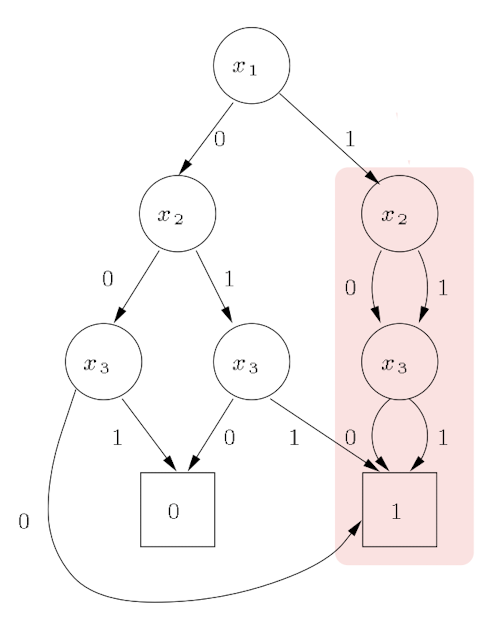
\includegraphics[scale=0.7]{obrazky-figures/bdd_a.png}
        \caption{BDD před kompresí cest.}
        \label{bdd_example_a}
    \end{subfigure}
    \vspace{\floatsep}
    \begin{subfigure}{.45\textwidth}
        \centering
        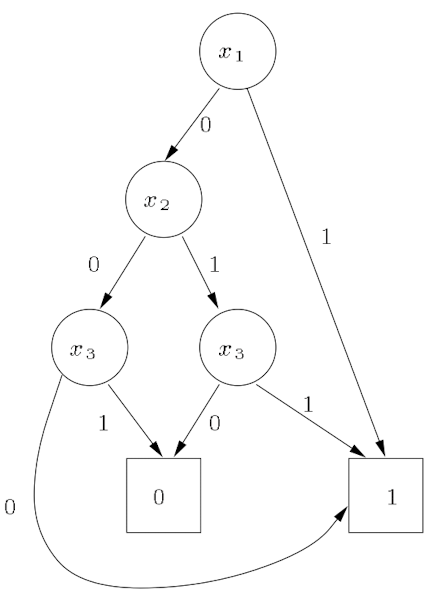
\includegraphics[scale=0.7]{obrazky-figures/bdd_b.png}
        \caption{BDD po kompresi cest.}
        \label{bdd_example_b}
    \end{subfigure}
    \caption{Ukázka možného BDD pro booleovskou funkci $ \Phi (x_1,x_2,x_3) \equiv x_1 \vee (x_2 \Leftrightarrow x_2) $.}
    \label{bdd_example}
\end{figure}

%*TODO možná BDD algoritmy a presna definice BDD*

\paragraph{BDD reprezentace automatu.} Jak už jsme zmínili, použití klasické reprezentace automatu vede k exponenciální velikosti abecedy, vzhledem k počtu proměnných ve formuli, tedy každý stav může mít až exponenciálně přechodů, což je značně neefektivní. Nejprve uvažme BDD reprezentaci automatu, při které jedno BDD kóduje množinu $ \{ (r,a,s) \mid r \rightarrow^a s \} $, kde $r,s$ jsou stavy a $a \in \mathbb{B}^k$ je symbol, což odpovídá celému automatu. Taková reprezentace vyžaduje zvolit vhodné kódování stavů. Výše uvedený přístup je také používán v symbolickém model checkingu. Například Kripkeho struktura $M=(S,I,R,L)$ nad atomickými pozorováními $AP = \{ p,q,r \} $, kde $S= \{ s_1,s_2,s_3 \}$ je konečná množina stavů, $ I \subseteq S = \{ s_1 \} $ je množina počátečních stavů, $R \subseteq S \times S = \{ (s_1,s_2),(s_2,s_3),(s_1,s_3),(s_3,s_3) \} $ je přechodová relace a $ L : 2^{AP} $ je označovací funkce. Pokud máme $n$ stavů, pak počet proměnných v~BDD na zakódování těchto stavů je $m = \lceil \log_2n \rceil $. V našem příkladě tedy potřebujeme dvě proměnnné $v_1,v_2$. Formule $\phi_S(v_1,v_2) =\neg v_1 \vee (v_1 \wedge \neg v_2) $ reprezentuje množinu stavů $S$. Toto zakódování říká, že stav $s_1$, $s_2$, $s_3$ odpovídá postupně $\phi_S(00)$, $\phi_S(01)$, $\phi_S(10)$. Dále každé atomické pozorování má vlastní BDD, které představuje funkci, jenž nám dává informaci v~jakých stavech dané pozorování platí. Bohužel výše popsaná reprezentace není vhodná pro některé základní automatové operace, které v rozhodovací procedůře potřebujeme, jako je minimalizace nebo determinizace. Samotná reprezentace není kanonická, protože neexistují žádná pravidla pro zakódování stavů. Vidíme, že reprezentace pomocí jednoho BDD není ideální pro automatové operace, tím pádem budeme chtít jinou datovou strukturu, která bude podporovat efektivní automatové operace.

\paragraph{SMTBDD.} Výše uvedený problém budeme řešit pomocí \textit{shared, multi-terminal BDD}. Rozdíl oproti klasickým je, že listy nejsou booleovské $0$,$1$, ale odpovídají stavům automatu. Každý stav je asociován k jednomu BDD, ovšem jednotlivá BDD spolu navzájem sdílejí uzly. Například formule $\exists p,q: p \neq q \wedge p \in X \cap Y \wedge q \in X \cap Y $ (neformálně, průnik $X$ a $Y$ obsahuje více než jeden element), je reprezentována automatem $M$ na obrázku~\ref{mona_aut}, kde je každý stav, $r,s,t$, definován pomocí informace jestli je koncový a ukazatele na svůj počáteční BDD uzel, určující jeho přechodovou relaci. Datová struktura ještě obsahuje jeden ukazatel na počáteční stav celého automatu. Jazyk, který automat přijíma je $L(M)= (\binom{0}{0}+\binom{0}{1}+\binom{1}{0})^*\binom{1}{1}(\binom{0}{0}+\binom{0}{1}+\binom{1}{0})^*\binom{1}{1} (\binom{0}{0}+\binom{0}{1}+\binom{1}{0}+\binom{1}{1})^* $.

\begin{figure}
    \centering
    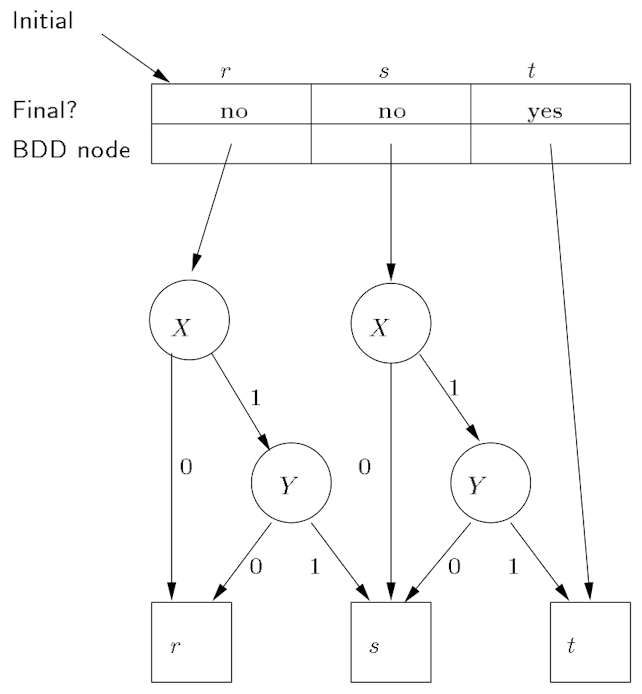
\includegraphics[scale=0.5]{obrazky-figures/mona_aut.png}
    \caption{Mona automat pro formuli $\exists p,q: p \neq q \wedge p \in X \cap Y \wedge q \in X \cap Y $.}
    \label{mona_aut}
\end{figure}

\paragraph{Interpretace řetězců.} Tato část pojednává o tom, jak mapujeme řetězce automatu na přiřazení hodnot proměnných v logice. Jako příklad uvažme WS1S formuli $ \phi \equiv P = Q $ a interpretaci $ P = \{ 1,3 \} $, $ Q = \{ 2,3 \} $. Tato interpretace je reprezentována řetězcem nad abecedou $ \mathbb{B}^2$:

\begin{center}
    \begin{tabular}{ |c|c|c|c|c|c|c|c| } 
        \hline
          & -1 & 0 & 1 & 2 & 3 & 4 & 5 \\
        \hline
        $P$ & 0 & 0 & 1 & 0 & 1 & 0 & 0 \\ 
        $Q$ & 0 & 0 & 0 & 1 & 1 & 0 & 0 \\ 
        \hline
    \end{tabular}
\end{center}

Zde první řádek odpovídá přirozeným číslům, kromě první pozice, která je vyhrazena pro booleovské proměnné, jenž budou vysvětleny v zápětí. Druhý řádek odpovídá prezenci hodnot z prvního řádku v proměnné $P$. Třetí řádek je analogický k druhému, akorát představuje proměnnou $Q$. Pokud označíme tento řetězec jako $w$, můžeme psát, že $ w \nvDash \phi $. Všimněme si, že existuje mnoho dalších řetezců, které popisují tuto interpretaci, protože když přidáme neomezený počet symbolu $ \binom{0}{0} $, interpretace zůstane totožná. Obecně pro $k$~proměnných formule $\phi$ definuje jazyk $L(\phi)=\{ w \mid w \vDash \phi \} $ nad abecedou $ \mathbb{B}^k $. 

Přirozená čísla se v klasickém přístupu kódují shodně jako množiny, ale navíc s omezením na počet prvků množiny roven $1$ (např. $a = 1 \wedge singleton(a)$). V Moně se tento přístup liší, a to tak, že tyto proměnné jsou neprázdné množiny, které jsou interpretovány jako jejich nejmenší hodnota. Booleovské proměné jsou zakodovány v řetězci tak, že je na jeho začátek přidána speciální pozice, značená $-1$. Jestliže je proměnná typu bool, pak je na tuto pozici vložena $0,1$, pokud je proměnná ohodnocena jako postupně $true,false$. Vidíme, že když nepoužíváme negaci, je jazyk automatů bez prázdného řetězce, ikdyž by ve formuli nebyly globální proměnné. Další rozdíl mezi klasickým přístupem a Mona přístupem je použití výrazně většího počtu speciálních automatů pro příslušné logické operace, aby se nemuselo často zjednodušovat formule (např. převádět každou implikaci na negaci a disjunkci). 

\subsection{Dagifikace formulí}

Mona je rozdělena na front-end a back-end. Front-end se stará o načítání, syntaktickou a sémantickou analýzu vstupní formule a vytvoření AST (\textit{abstraktního syntaktického stromu}), jehož vnitřní uzly jsou podporované automatové operace a listy jsou atomické formule. Back-end poté induktivně provádí tyto automatové operace a nakonec vytvoří automat korespondující k dané formuli. V dřívějších verzích nástroje se přímo z AST vytvořil kódový strom a z něj se postupně generovaly automaty. Lze ovšem vypozorovat, že v kódovém stromu se nachází mnoho stejných podstromů modulo přejmenování proměnných. Výše zmíněný fakt vedl k tomu, že byla vytvořena tato optimalizace a shodné podstromy modulo přejmenování se vytváří pouze jednou. To má za následek, že kód se již nevytvoří ze stromu, ale z OAG (\textit{orientovaného acyklického grafu}) a již vytvořené automaty se použijí vícekrát. Kódové stromy mohou být například ve formě $ mk\_basic\_less(i,j) $, $ mk\_product(C,C',op) $, $ mk\_project(i,C) $, kde $i,j$ jsou indexy BDD proměnných, $op$ je booleovská funkce s dvěma proměnnými a $C,C'$ jsou kódové stromy. Pro ilustraci uvažme formuli $ \exists q: p < q \wedge q < r $. Předpokládejme, že proměnné $p,q,r$ mají postupně index 1,2,3, kde index udává pořadí řazení proměnných, pak je tato formule transformována na kódový strom $ mk\_project(2, mk\_product(mk\_less(1,2),$ $mk\_less(2,3), \wedge )) $. Na tomto stromě můžeme vidět, že obsahuje dva izomorfní podstromy, ze kterých by se později dvakrát počítal stejný automat. Automat $A$ pro $mk\_less(1,2)$ je identický s automatem $A'$ pro  $mk\_less(2,3)$ modulo přejmenování proměnných. Ukázka transformace z kódového stromu na OAG je na obrázku \ref{dagifikace}. Lze nahlédnout, že listové uzly jsou izomorfní modulo přejmenování, tudíž se sjednotí v jeden uzel a obě hrany jsou označeny použitým přejmenováním. Obecně bychom chtěli přejmenovat indexy v $A$ kdykoliv kdy potřebujeme $A'$. Touto optimalizací můžeme podstatně zlepšit celkovou rychlost programu, protože přejmenování indexů je lineární operace, zatím co konstrukce $A'$ je většinou časově složitější. Řekneme, že kódový strom $C$ je ekvivalentní $C'$, pokud existuje přejmenování proměnných, které zachovává pořadí, v $C'$ takové, že z $C'$ se stane $C$.

\begin{figure}
    \centering
    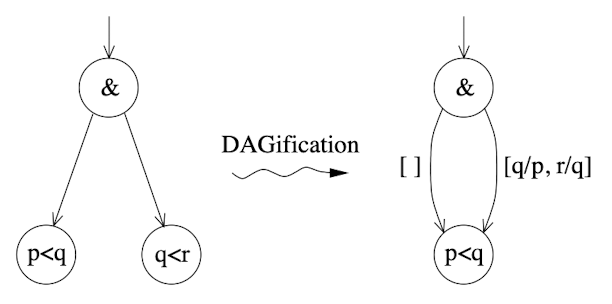
\includegraphics[scale=0.6]{obrazky-figures/dagifikace.png}
    \caption{Transformace formule $ \exists q: p < q \wedge q < r $ z kódového stromu na OAG.}
    \label{dagifikace}
\end{figure}

Z uvedené ekvivalence plyne, že uvažovaná formule splňuje tuto ekvivalenci a tím pádem automat může být znovupoužit. Výhoda BDD reprezentace je, že jestliže dva kódové stromy splňují výše uvedenou ekvivalenci, pak mají identické BDD až na listové uzly, kde každý má obecně jiné stavy do kterých může přejít. Pokud bychom ve výše zmíněné formuli zachovali indexy a změnili ji do podoby $ \exists q: p < q \wedge r < q $, pak definice ekvivalence není splněna (tedy dvě BDD jsou různé pro obě atomické formule) a dagifikace se neprovede. Cílem je vytvořit OAG, který vznikne z kódového stromu pomocí odstranění ekvivalentních podstromů. Celkový čas potřebný pro tuto procedůru je ovšem kvadratický, protože jak již bylo zmíněno, je potřeba lineární čas na samotné přejmenování a další lineární čas zabere výpočet relace ekvivalence. Z toho důvodu je dagifikace omezena na podstromy o~maximálním počtu proměnných, který uživatel specifikuje pomocí parametru.

%*TODO možná obrázek kde budou ty ruzné BDD při (ne)zachování pořadí*

\subsection{Restrikce formulí}

%* TODO z man\_str23, samostatneho clanku a impl secr *

Motivací pro vytvoření této optimalizace je problém zakódování prvořádových proměnných, tedy jak efektivněji vyjádřit prvořádové proměnné pomocí druhořádových. Hlavní myšlenka restrikcí je, že k hlavní formuli $\phi$ přidružíme restrikci $\phi_R$, kde $\phi_R$ je také formule. Pokud je $\phi$ formule s restrikcí, pak $\phi_R$ je různá od $true$, jinak pokud neobsahuje restrikci, pak $\phi_R$ je $true$. $\phi$ můžeme dále uvažovat pouze pokud $\phi_R$ platí. Například nechť $\phi = \exists x: x \cup y = \emptyset $ a $\phi_R=x\subseteq y$, pak vytvořený automat je ekvivalentní s automatem pro formuli $\phi'= \exists x: x \cup y \wedge x\subseteq y$. Nyní budou popsány různé způsoby řešení tohoto problému, tak jak postupem času byly implementovány v nástroji Mona, včetně zde naznačených restrikcí.

\paragraph{Ad hoc strategie a konjunktivní sémantika.} Nejjednodušší přístup pro vyjádření prvořádových proměnných je \textit{ad hoc strategie}, což je klasický přístup, kdy s proměnnou $p$ zacházíme jako s druhořádovou proměnnou, tedy množinou o jednom prvku a v místě vzniku $p$ (hlavní formule, pokud je volná proměnná nebo místo kde vzniká kvantifikováním, pokud je vázaná) k ní přidáme konjunkcí singleton predikát. Tato strategie znamená, že sémantika formule obsahující $p$ není robustní, protože její význam na interpretacích řetězců jazyka $w$ nesplňujících $singleton(p)$ není dobře definován. Ikdyby byl tento predikát přidán ke každému výskytu $p$ v atomických formulích tak, jak již bylo rozebíráno v předchozí kapitole, sémantika této reprezentace není uzavřená vůči komplementu. Řešení je přidat konjunkci s restrikcí ke každé podformuli formule $p$, čemuž říkáme \textit{konjunktivní sématika}. V tomto případě má každý řetězec $w$ korektní sémantiku, jelikož po případné negaci ve vnořené formuli obsahující prvořádové proměnné $p_i$ následuje konjunkce se singleton automatem pro všechny proměnné $p_i$, tedy tyto proměnné zůstanou nadále interpretované jako prvořádové, a to po celou dobu výpočtu. Praktický problém s tímto přístupem je to, že se provede navíc velké množství operací minimalizace a průniku. Konkrétně, pro každý automat $A$ reprezentující podformuli $\phi$ a každou volnou proměnnou $P_i$, automat reprezentující $singleton(P_i)$, musí být konjunkcí přidán k $A$. Tyto operace, provedené navíc oproti \textit{ad hoc} přístupu, zpomalí rozhodovací procedůru alespoň dvojnásobně. Komplementace, která je rychlá operace, protože automaty jsou deterministické a úplné, sestává z prohození koncových a nekoncových stavů, ovšem nyní by obsahovala navíc minimalizaci a průnik. Stějně tak operace průniku by provedla navíc alespoň jednou minimalizaci a průnik. Z těchto důvodu se v Moně, před implementací restrikcí, používal \textit{ad hoc} přístup s tím, že se singleton vlastnost proměnných přidala k atomickým formulím, kde se daná proměnná vyskytovala a~k formuli, kde příslušná proměnná vznikla. Add hoc sématiku můžeme nadefinovat pomocí významové funkce $ \llbracket \phi \rrbracket^{ah} $ takto:

\begin{equation}
    \llbracket \neg \phi' \rrbracket^{ah}w = \neg \llbracket \phi' \rrbracket^{ah}w
\end{equation}
\begin{equation}
    \llbracket \phi' \wedge \phi'' \rrbracket^{ah}w = \llbracket \phi' \rrbracket^{ah}w \wedge \llbracket \phi'' \rrbracket^{ah}w
\end{equation}
\begin{equation}
    \llbracket \exists P^i \text{ } where \text{ } \rho: \phi' \rrbracket^{ah}w = 
    \begin{cases}
        1 & \text{pokud}\ \exists M: \llbracket \phi' \rrbracket^{ah} w[P^i \mapsto M]=1 \wedge \llbracket \rho^* (P^i) \rrbracket^{ah}=1 \\
        0 & \text{pokud}\ \forall M: \llbracket \phi' \rrbracket^{ah} w[P^i \mapsto M]=0 \vee \llbracket \rho^* (P^i) \rrbracket^{ah}=0
    \end{cases}
\end{equation}
\begin{equation}
    \label{ah_sub}
    \llbracket P^i \subseteq P^j \rrbracket^{ah}w=
    \begin{cases}
        1 & \text{pokud}\ w \vDash P^i \subseteq P^j \wedge \llbracket \rho^* (P^i \subseteq P^j) \rrbracket^{ah}w=1  \\
        0 & \text{pokud}\ w \nvDash P^i \subseteq P^j \vee \llbracket \rho^* (P^i \subseteq P^j) \rrbracket^{ah}w=0
    \end{cases}
\end{equation}

kde $\rho^*$ jsou všechny restrikce relevantních proměnných (bude detailněji vysvětleno v~následujícím odstavci). Například intuitivní význam rovnice \ref{ah_sub} je takový, že $true$ vrátí, pokud $w$ je modelem a všechny relevantní restrikce jsou splněny, naopak $false$ vrátí, pokud $w$ není modelem nebo nějaká relevantní restrikce není splněna. Sémantika na ostatních základních atomických formulích se definuje analogicky. Konjunktivní sémantika se definuje stejně, akorát jsou restrikce aplikovány také na operátory $\wedge$ a $\neg$.

\paragraph{Restrikce a tří-hodnotová sémantika.} Mona si mírně upravila syntax WS1S, a to tak, že umožňuje vytvářet restrikce explicitně. Existenční kvantifikace poté vypadá jako $\exists P^i$ $ where $ $\rho: \phi'$, kde $\rho$ je restrikce proměnné $P^i$, značeno jako $\rho (P^i)$. Předpokládejme, že každá $P^i$ má nějakou restrikci (pokud by neměla, tak $\rho (P^i)=true$). Dále řekněme, že v~$\rho (P^i)$ je proměnná $P^i$ \textit{$\rho$-vázaná}. Proměnná $P^i$ je \textit{existenčně vázaná} v $\rho (P^i)$ i v $\phi'$. Výskyt proměnné $P^i$ je \textit{volný} v konvenční části $\phi$, pokud $P^i$ je volná v $\phi$ v běžném významu, kde $\phi$ je považována za nezávislou formuli a výskyt není v rámci restrikce existenční kvantifikace v rámci $\phi$. \textit{Relevantní proměnné} formule $\phi$, $RV(\phi)$, je nejmenší množina proměnných $P$ taková, že existuje výskyt $P$, který není $\rho$-vázaný a zároveň je volný v konvenční části $\phi$ nebo volný v konvenční části $\rho(P')$, kde $P' \in RV(\phi)$. Dále definujme \textit{indukovanou restrikci} $\rho^*(\phi)$ jako $\rho^*(\phi)= \wedge_{P^i\in RV(\phi)} $, což, neformálně řečeno, je konjunkce restrikcí relevantních proměnných. Nechť $\mathbb{B}^- = \mathbb{B} \cup \{ \perp \} $ je \textit{rozšířená booleovská doména}. Symbol $\perp$ bude označovat situaci, kdy existuje restrikce, která neplatí. Booleovské operátory ($\wedge^3$ a $\neg^3$ jsou definovány na $ \mathbb{B}^- \times \mathbb{B}^- $ obvyklým způsobem, navíc je situace s $\perp$, kdy je vždy výsledek $\perp$) a tří-hodnotová sémantika jsou definovány následovně:


\begin{center}
    \begin{tabular}{c|c}
        $\neg^3$ &  \\ \hline
        $\perp$ & $\perp$ \\ 
        $-$ & $+$ \\ 
        $+$ & $-$ \\ 
    \end{tabular}
    \quad
    \begin{tabular}{c|ccc}
        $\wedge^3$ & $\perp$ & $-$ & $+$ \\ \hline
        $\perp$ & $\perp$ & $\perp$ & $\perp$ \\ 
        $-$ & $\perp$ & $-$ & $-$ \\ 
        $+$ & $\perp$ & $-$ & $+$ \\ 
    \end{tabular}
\end{center}

\begin{equation}
    \llbracket \neg \phi' \rrbracket^{3}w = \neg^3 \llbracket \phi' \rrbracket^{3}w
\end{equation}
\begin{equation}
    \llbracket \phi' \wedge \phi'' \rrbracket^{3}w = \llbracket \phi' \rrbracket^{3}w \wedge^3 \llbracket \phi'' \rrbracket^{3}w
\end{equation}
\begin{equation}
    \llbracket \exists P^i \text{ } where \text{ } \rho: \phi' \rrbracket^{3}w = 
    \begin{cases}
        1 & \text{pokud}\ \exists M: \llbracket \phi' \rrbracket^{3} w[P^i \mapsto M]=1 \\
        0 & \text{pokud}\ \forall M: \llbracket \phi' \rrbracket^{3} w[P^i \mapsto M] \neq 1 \wedge \exists M: \llbracket \phi' \rrbracket^{3} w[P^i \mapsto M]=0 \\
        \perp & \text{pokud}\ \forall M: \llbracket \phi' \rrbracket^{3} w[P^i \mapsto M]= \perp
    \end{cases}
\end{equation}
\begin{equation}
    \label{tri_h_s_sub}
    \llbracket P^i \subseteq P^j \rrbracket^{3}w=
    \begin{cases}
        1 & \text{pokud}\ w \vDash P^i \subseteq P^j \wedge \llbracket \rho^* (P^i \subseteq P^j) \rrbracket^{3}w=1  \\
        0 & \text{pokud}\ w \nvDash P^i \subseteq P^j \wedge \llbracket \rho^* (P^i \subseteq P^j) \rrbracket^{3}=1 \\
        \perp & \text{pokud}\ \llbracket \rho^* (P^i \subseteq P^j) \rrbracket^{3} \neq 1
    \end{cases}
\end{equation}

Zde například rovnice \ref{tri_h_s_sub} neformálně říká, že pokud je $w$ model a všechny relevantní restrikce jsou splněny, pak vrací $true$, jinak pokud $w$ není model a všechny relevantní restrikce jsou splněny, vrací $false$, jinak pokud nějaká relevantní restrikce není splněna, vrací $\perp$. Následně můžeme sestrojit tři ekvivalence:

\begin{equation}
    \label{tri_h_s_final1}
    w \nvDash \rho (P^i) \text{ pro nějaké } P^i \in RV(\phi) \Leftrightarrow w \nvDash \rho^* (\phi) \Leftrightarrow \llbracket \phi \rrbracket^3w = \perp
\end{equation}
\begin{equation}
    \label{tri_h_s_final2}
    w \vDash \phi \wedge \rho^* (\phi) \Leftrightarrow \llbracket \phi \rrbracket^3w = 1
\end{equation}
\begin{equation}
    \label{tri_h_s_final3}
    w \vDash \neg \phi \wedge \rho^* (\phi) \Leftrightarrow \llbracket \phi \rrbracket^3w = 0
\end{equation}

Ekvivalence \ref{tri_h_s_final1} hovoří o situaci, kdy je porušena nějaká restrikce, ekvivalence \ref{tri_h_s_final2} o~případu, kdy je splněna formule i restrikce a konečně ekvivalence \ref{tri_h_s_final3} o situaci, kdy není splněna formule, ale je splněna restrikce. Pokud upravíme původní algoritmus tak, aby reflektoval tří-hodnotovou sémantiku, získáme výsledný algoritmus tří-hodnotové rozhodovací procedůry pro WS1S.

\chapter{Nová rozhodovací procedůra}
\label{2_nova_roz_proc}

Tato kapitola představí novou reprezentaci automatů a přizpůsobené automatové algoritmy pro efektivní práci s touto reprezentací, což představuje hlavní konceptuální přínos této práce.

\section{Hlavní myšlenka}

Hlavní změna v nové rozhodovací procedůře je, že BDD uzly použité k reprezentaci přechodů integrujeme přímo do automatu jako stavy. Toto lze snadno, protože protože BDD procedůry jsou podobné automatovým. Abychom docílili funcionality BDD, kde jsou k~uzlům přidruženy proměnné, musíme v automatu použít skip hrany místo běžných hran. Běžný konečný automat tedy upravíme tak, že změníme definici konečné množiny pravidel, což je relace $R \subseteq Q \times (\Sigma \cup \{ \epsilon \}) \times Q $ do podoby $R \subseteq Q \times (\Sigma \cup \{ \epsilon \}) \times \mathbb{N} \times Q$, kde nová relace přidává ke každému pravidlu jedno kladné číslo, které značí délku hrany, což odpovídá počtu přeskočených hran $+ 1$. Poznamenejme, že délka hrany $1$ je speciální případ odpovídající běžným hranám. Automat se skip hranou ze stavu $p$ do stavu $r$ s přechodovým symbolem $a$ a délkou hrany $n$, kde $n>0$, přijme $a$, poté $n-1$-krát všechny symboly abecedy a následně skončí ve stavu $r$ (na obrázku \ref{skip_trans} vidíme ukázku obecné skip hrany a korespondující běžné hrany).

\begin{figure}[h]
    \usetikzlibrary{calc}
    \usetikzlibrary{decorations.pathreplacing}
    \centering
    \begin{subfigure}{.29\textwidth}
        \centering
        \begin{tikzpicture}[shorten >=1pt,node distance=2cm,on grid,auto] 
            \node[state,initial, initial text= ] (Q_1)   {$p$}; 
            \node[state,accepting](Q_2) [right=of Q_1] {$r$};
            \path[->]
                (Q_1) edge  node  {$a$/$n$} (Q_2);
        \end{tikzpicture}
        \caption{}
        \label{skip_trans1}
    \end{subfigure}
    \hfil
    \begin{subfigure}{.7\textwidth}
        \centering
        \begin{tikzpicture}[shorten >=1pt,node distance=2cm,on grid,auto] 
            \node[state,initial, initial text= ] (Q_0)   {$p$}; 
            \node[state] (Q_1) [right=of Q_0] {$q_0$};
            \node[state] (Q_2) [right=of Q_1] {$q_1$};
            \node[state] (Q_3) [right=of Q_2] {$q_{n-2}$};
            \node[state,accepting] (Q_4) [right=of Q_3] {$r$};
            \node at ($(Q_2)!0.5!(Q_3)$) {$\cdots$};
            \node at ($(Q_2)!0.3!(Q_3)$) {$\cdot$};
            \node at ($(Q_2)!0.7!(Q_3)$) {$\cdot$};
            \path[->]
                (Q_0) edge  node  {$a$/$1$} (Q_1)
                (Q_1) edge [bend left] node  {$0$/$1$} (Q_2)
                (Q_1) edge [bend right] node  {$1$/$1$} (Q_2)
                (Q_3) edge [bend left] node  {$0$/$1$} (Q_4)
                (Q_3) edge [bend right] node  {$1$/$1$} (Q_4);
                
            \draw[decorate,decoration={brace,amplitude=10pt,mirror}] (Q_1.south) -- (Q_4.south) node[midway,below=0,yshift=-15pt] {$n-1$};
        \end{tikzpicture}
        \caption{}
        \label{skip_trans2}
    \end{subfigure}
    \caption{Porovnání obecné skip hrany s přechodovým symbolem $a$ o délce $n$ (obrázek~\ref{skip_trans1}) a jí ekvivalentním běžným hranám (obrázek \ref{skip_trans2}). Notaci na hranách $a/n$ interpretujeme jako přechodový symbol $a$ a délku hrany $n$.}
    \label{skip_trans}
\end{figure}

\begin{figure}
    \centering
    \begin{subfigure}{.3\textwidth}
        \centering
        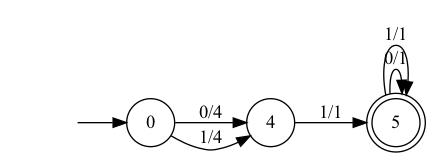
\includegraphics[scale=0.3]{obrazky-figures/skip_adv_in.png}
        \caption{Množina proměnných $\{ X \}$ a formule $3 \in X$.}
        \label{skip_adv_in}
    \end{subfigure}%
    \hfil
    \begin{subfigure}{.65\textwidth}
        \centering
        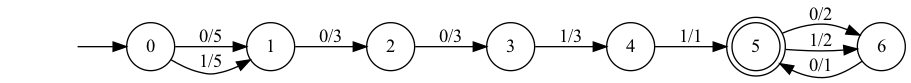
\includegraphics[scale=0.3]{obrazky-figures/skip_adv_set.png}
        \caption{Množina proměnných $\{ X,Y,Z \}$ a formule $Z=\{ 2,3 \}$.}
        \label{skip_adv_set}
    \end{subfigure}
    \caption{Nastínění možných výhod přechodů pomocí skip hran oproti pomocí BDD. BDD přechody by museli přidat stav vždy po jednom přiřazení do všech proměnných, což v terminologii skip hran znamená maximálnní délku hrany rovnu počtu proměnných a před přiřazením do první proměnné musí existovat stav.}
    \label{skip_adv}
\end{figure}

Se skip hranami lze zajít dál než s BDD, protože umožňují neomezeně dlouhý skok, tedy oproti BDD kódování přechodů je výhoda, že skip hrany mohou přeskočit i několik stavů automatu. BDD dokáží přiřadit booleovské ohodnocení každé proměnné ve formuli a pokud na její hodnotě nezáleží, tak nevytvoří vnitřní uzel, ale pokud bychom měli formuli, kde například mohou mít $n$-krát všechny proměnné libovolnou hodnotu, pak sice BDD nebude mít žádný vnitřní uzel, ale musí se vytvořit $n$ automatových stavů, protože pomocí BDD nelze říct, že proměnné přeskočím vícekrát. Naopak u skip hran může být délka hrany větší něž počet proměnných a tedy není nutné vytvářet zbytečné stavy. Ukázka takové formule je na obrázku \ref{skip_adv}. Díky této vlastnosti se také ušetří stavy, pokud přiřazujeme do jedné proměnné a na ostatních nám nezáleží, protože vždy po každém jednom přiřazení do všech proměnných se nevytvoří stav, pokud to není nutné (viz příklad z obrázku \ref{skip_adv}). Zmíníme také, že čistě automatová reprezentace, namísto kombinace automatů a BDD, je flexibilnější, lze do ní lépe vidět a umožňuje navíc třeba nedeterminismus nebo reverzaci.

\section{Automatové algoritmy}

V následující části budou popsány vybrané automatové algoritmy potřebné pro rozhodování WS1S upravené tak, aby efektivně pracovaly s představenou reprezentací. Zde je výčet často používaných symbolů a vysvětlení jejich intuitivního významu:

\begin{itemize}
    \item $s_a$ / $S_a$ znamená aktuální stav / množinu stavů
    \item $s_f$ / $S_f$ znamená následující stav / množinu stavů
    \item $s_i$ / $S_i$ znamená mezistav / množinu mezistavů
    \item $symb$ znamená aktuální přechodový symbol
\end{itemize}

\subsection{Průnik}

Průnik je běžná automatová operace, proto jsme se rozhodli, že tento algoritmus popíšeme zjednodušeně a dáme důraz na odlišnosti při práci se skip hranami, což vizualizuje algoritmus \ref{intersection_core}. 

\begin{algorithm}[t]
    \caption{Průnik automatů se skip hranami}
    \label{intersection_core}
        \begin{algorithmic}[1]
            \Procedure{intersection}{$aut_1,aut_2$}
                \State $result \gets emptyAutomaton()$
                \State $q \gets emptyVector()$
                \For{$init_1$ \textbf{in} $aut_1.initial\_states$}
                    \For{$init_2$ \textbf{in} $aut_2.initial\_states$}
                        \State $q.push((init_1,init_2))$
                    \EndFor
                \EndFor
                \While{$q$ is not empty}
                    \State $s_{a_1},s_{a_2} \gets q.pop()$
                    \While{exists next move from $s_{a_1},s_{a_2}$}
                        \State $S_{f_1},S_{f_2},symb \gets getNextMove()$
                        \For{$s_{f_1}$ \textbf{in} $S_{f_1}$}
                            \For{$s_{f_2}$ \textbf{in} $S_{f_2}$}
                                \State $addInnersInter(aut_1,aut_2,s_{a_1},s_{a_2},s_{f_1},s_{f_2},symb)$
                                \State $createResultStateAndTrans()$
                            \EndFor
                        \EndFor
                        \State $addResultTrans()$
                    \EndWhile
                \EndWhile
                \State \Return result
            \EndProcedure
        \end{algorithmic}
\end{algorithm}

\paragraph{Společný rámec průniku.} Nejprve vytvoříme všechny dvojice iniciálních stavů obou vstupních automatů a umístíme je do vektoru. Následně dokud je vektor neprázdný, vytahujeme z něj dvojice stavů. Podmínka na řádku $11$ říká, že ze stavu $s_{a_1}$ existuje přechod v $aut_1$ do nějakého stavu $s_{f_1}$ přes symbol $symb$ a ze stavu $s_{a_2}$ je možné v $aut_2$ přejít přes symbol $symb$ do stavu $s_{f_2}$. Funkce $getNextMove$ je obdoba výše uvedené podmínky, ovšem nevrací binární hodnotu, ale množinu všech $s_{f_1}$ (značeno jako $S_{f_1}$) a všechny $s_{f_2}$ (označíme jako $S_{f_2}$). Procedůra $createResultStateAndTrans$ vytvoří přechod přes aktuální symbol a~nový stav výsledného automatu, pokud je aktuální dvojice stavů viděna poprvé a také pokud jsou oba stavy koncové, nastaví nový stav jako koncový a $addResultTrans$ přidá nově vzniklé přechody a stavy do výsledného automatu. Ve funkci $addInnersInter$ se odehrává to nejpodstatnější, což je vypořádání se se skip hranami. Algoritmy \ref{add_inners_1} a \ref{add_inners_2} představují dvě nejefektivnější realizace, které jsme implementovali.

\begin{algorithm}[t]
    \caption{Vytváření mezistavů během průniku (verze 1)}
    \label{add_inners_1}
        \begin{algorithmic}[1]
            \Procedure{addInnersInter}{$aut_1,aut_2,s_{a_1},s_{a_2},s_{f_1},s_{f_2},symb$}
                \State $jump_1 \gets getEdgeLen(s_{a_1},s_{f_1})$
                \State $jump_2 \gets getEdgeLen(s_{a_2},s_{f_2})$
                \If{$jump_1 < jump_2$}
                    \State $aut_2.remove\_trans(s_{a_2}, symb, s_{f_2})$
                    \State $s_i \gets aut_2.add\_state()$
                    \State $aut_2.add\_trans(s_{a_2}, symb, s_i, jump_1)$
                    \State $aut_2.add\_one\_jump\_trans(s_i,0,s_{f_2},jump_2 - jump_1)$
                    \State $aut_2.add\_one\_jump\_trans(s_i,1,s_{f_2},jump_2 - jump_1)$
                    \State $s_{f_2} \gets s_i$
                \EndIf
                \If{$jump_1 > jump_2$}
                    \State $aut_1.remove\_trans(s_{a_1}, symb, s_{f_1})$
                    \State $s_i \gets aut_1.add\_state()$
                    \State $aut_1.add\_trans(s_{a_1}, symb, s_i, jump_2)$
                    \State $aut_1.add\_one\_jump\_trans(s_i,0,s_{f_1},jump_1 - jump_2)$
                    \State $aut_1.add\_one\_jump\_trans(s_i,1,s_{f_1},jump_1 - jump_2)$
                    \State $s_{f_1} \gets s_i$
                \EndIf
            \EndProcedure
        \end{algorithmic}
\end{algorithm}

\paragraph{Princip vytváření mezistavů pro průnik.} Princip vytváření mezistavů je následující. Nechť máme aktuální dvojici stavů $s_{a_1}$ a $s_{a_2}$, která přes symbol $symb$ přejde do stavů $s_{f_1}$ a $s_{f_2}$ (index $1$ značí stavy v automatu $aut_1$, index $2$ analogicky, ale v $aut_2$). Pokud je délka hrany z $s_{a_1}$ do $s_{f_1}$ rovna délce z $s_{a_2}$ do $s_{f_2}$, pak je vše v pořádku a nic nemusíme řešit. V~případě, že například délka hrany v prvním automatu je kratší, je nutné přidat mezistav $s_{i_2}$ do druhého automatu, a to tak, že hranu z $s_{a_2}$ do $s_{f_2}$ odstraníme, přidáme hranu začínající v $s_{a_2}$ a jdoucí do $s_{i_2}$ přes symbol $symb$ o stejné délce jakou má hrana $s_{a_1}$ až $s_{f_1}$. Abychom odstraněnou hranu nahradili kompletně, musíme ještě přidat dvě hrany z $s_{i_2}$ do $s_{f_2}$ přes oba symboly $0,1$, které budou mít délku původní hrany sníženou o vzdálenost z $s_{a_1}$ do $s_{f_1}$. Dále budeme zpracovávat místo původní dvojice $fs_1$, $fs_2$, dvojici $s_{f_1}$, $s_{i_2}$. 

\paragraph{Algoritmus vytváření mezistavů pro průnik (verze 1).} Funkce $getEdgeLen$ vrátí délku hrany mezi dvěma stavy předanými jako její parametry. Metody $remove\_trans$ a~$add\_trans$ jsou celkem přímočaré, a tedy odstraní či přidají přechod z prvního parametru, přes symbol z druhého parametru do stavu v třetím parametru. Pokud má $add\_trans$ navíc čtvrtý parametr, znamená to, že nastavíme délku přidané hrany na jeho hodnotu, jinak se použije implicitní délka hrany, která je $1$. Metoda $add\_one\_jump\_trans$ má identické parametry jako $add\_trans$, ale nevytvoří jednu hranu, nýbrž délka hrany $-1$ mezistavů a~z~počátečního stavu hrany do prvního mezistavu bude přechod se symbolem z parametrů metody a ostatní mezistavy (včetně koncového stavu hrany) budou propojeny oběma symboly abecedy $0,1$. Intuitivně, nevytvoří se jedna skip hrana, ale analogie této skip hrany s~použitím pouze běžných hran. Na první pohled to působí rozpačitě, protože by se mohlo zdát, že se naplno nevyužije potenciál skip hran, ovšem pokud na začátku algoritmu \ref{add_inners_1} dospějeme k situaci, že máme různé délky hran, tak se musí přidat mezistav a z něj kdybychom přidali pouze dvě hrany se symboly $0,1$ do cílových stavů, obdrželi bychom nežádocí větvění do šířky ve výsledném automatu. Ukázku tohoto efektu můžeme vidět na obrázku \ref{add_inners_1_img}. Abychom mohli skip hrany maximálně využít a zbavili se větvícího efektu, potřebujeme tyto mezistavy sdílet, pokud je to možné. Toho docílíme při použití druhé verze algoritmu $addInnersInter$ vyjádřeného algoritmem \ref{add_inners_2}.

\paragraph{Algoritmus vytváření mezistavů pro průnik (verze 2).} Zde se navíc nachází funkce $getInnerInter()$, která pokud již byl v automatu $aut_2$ (jestliže voláme z řádku $6$) či $aut_1$ (jestliže voláme z řádku $12$) vytvořen mezistav, ze kterého vede hrana délky $jump_2-jump_1$ (invokace z řádku $6$) nebo $jump_1-jump_2$ (invokace z řádku $12$) a směřuje do cílového stavu aktuálně zpracovávané hrany (přechodový symbol může být obecně různý), pak vrátí tento mezistav, jinak vytvoří nový mezistav, který oba symboly $0,1$ propojí s cílovým stavem této hrany. Tento přístup nám zajistí sdílení mezistavů a tím pádem již nebude docházet k~nežádoucímu větvení, což je demonstrováno na obrázku \ref{add_inners_2_img}. 

% TODO popsat nekde ze reduce je po interu, mozna v impl nebo exp

\begin{algorithm}
    \caption{Vytváření mezistavů během průniku (verze 2)}
    \label{add_inners_2}
        \begin{algorithmic}[1]
            \Procedure{addInnersInter}{$aut_1,aut_2,s_{a_1},s_{a_2},s_{f_1},s_{f_2},symb$}
                \State $jump_1 \gets getEdgeLen(s_{a_1},s_{f_1})$
                \State $jump_2 \gets getEdgeLen(s_{a_2},s_{f_2})$
                \If{$jump_1 < jump_2$}
                    \State $aut_2.remove\_trans(s_{a_2}, symb, s_{f_2})$
                    \State $s_{i} \gets getInnerInter()$
                    \State $aut_2.add\_trans(s_{a_2}, symb, s_{i}, jump_1)$
                    \State $s_{f_2} \gets s_{i}$
                \EndIf
                \If{$jump_1 > jump_2$}
                    \State $aut_1.remove\_trans(s_{a_1}, symb, s_{f_1})$
                    \State $s_{i} \gets getInnerInter()$
                    \State $aut_1.add\_trans(s_{a_1}, symb, s_{i}, jump_2)$
                    \State $s_{f_1} \gets s_{i}$
                \EndIf
            \EndProcedure
        \end{algorithmic}
\end{algorithm} 

\begin{figure}
    \centering
    \begin{subfigure}{.1\textwidth}
        \centering
        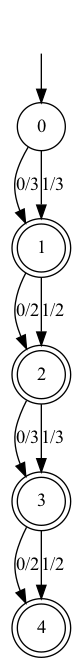
\includegraphics[scale=0.3]{obrazky-figures/add_inners_1_img_aut1.png}
        \caption{}
        \label{add_inners_1_img_aut1}
    \end{subfigure}
    \hfil
    \begin{subfigure}{.1\textwidth}
        \centering
        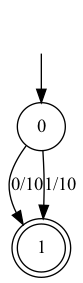
\includegraphics[scale=0.3]{obrazky-figures/add_inners_1_img_aut2.png}
        \caption{}
        \label{add_inners_1_img_aut2}
    \end{subfigure}
    \hfil
    \begin{subfigure}{.52\textwidth}
        \centering
        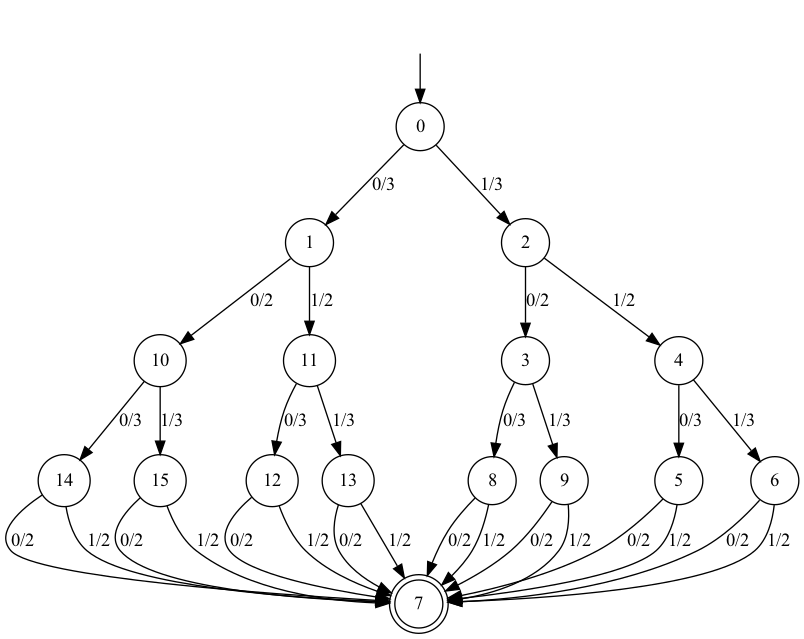
\includegraphics[scale=0.26]{obrazky-figures/add_inners_1_img_aut3.png}
        \caption{}
        \label{add_inners_1_img_aut3}
    \end{subfigure}
    \hfil
    \begin{subfigure}{0.24\textwidth}
        \centering
        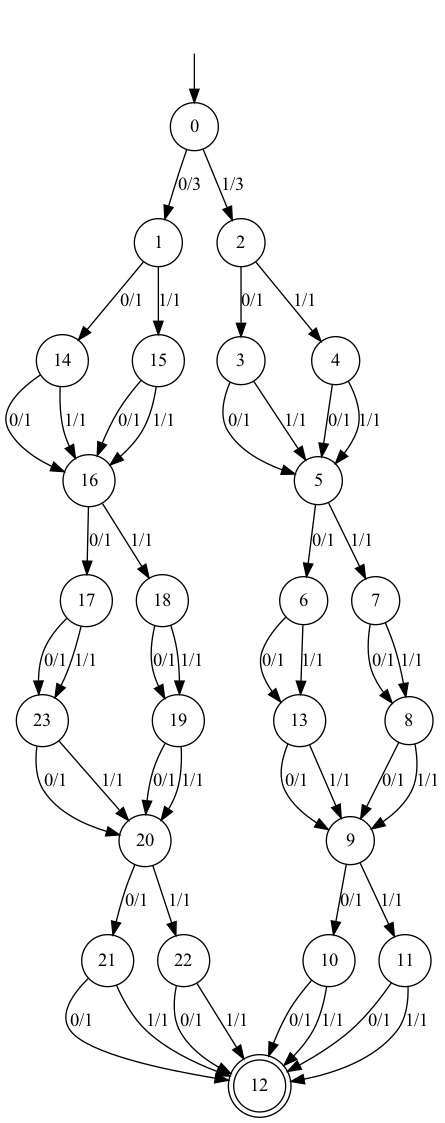
\includegraphics[scale=0.22]{obrazky-figures/add_inners_1_img_aut4.png}
        \caption{}
        \label{add_inners_1_img_aut4}
    \end{subfigure}
    \caption{Ukázka průniku automatů z obrázků \ref{add_inners_1_img_aut1} a \ref{add_inners_1_img_aut2} pomocí algortimu \ref{add_inners_1}. Obrázek~\ref{add_inners_1_img_aut3} vyobrazovává výsledek při použití maximálních možných délek skip hran (odpovídá použití metody $add\_trans$ místo $add\_one\_jump\_trans$ na řádcích $8,9,16,17$) a~obrázek~\ref{add_inners_1_img_aut4} ukazuje výsledek za přidávání pouze hran délky $1$ z mezistavů (tedy přesně dle algoritmu).}
    \label{add_inners_1_img}
\end{figure}

\begin{figure}
    \centering
    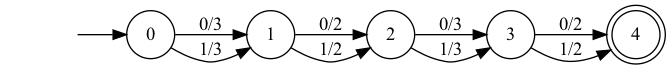
\includegraphics[scale=0.37]{obrazky-figures/add_inners_2_img_aut1.png}
    \caption{Vizualizace průniku automatů z obrázků \ref{add_inners_1_img_aut1} a \ref{add_inners_1_img_aut2} za použití algoritmu \ref{add_inners_2}.}
    \label{add_inners_2_img}
\end{figure}

\subsection{Determinizace}

Stejně jako průnik, tak i determinizace je klasická automatová operace, tudíž jsme se rozhodli pro zjednodušenou formu zápisu částí algoritmu, které jsou shodné pro automaty s~běžnými hranami i se skip hranami. Jedná se o jednu z nejčastěji využívaných operací, která se používá například během komplementace, projekce či minimalizace. Samotný pseudokód uvadíme v algoritmu \ref{deter_core}.

\paragraph{Společný rámec determinizace.} Algoritmus začne tím, že vloží do vektoru, sloužícího ke zpracovávání stavů, množinu iniciálních stavů automatu. Následně z vektoru vybere jednu položku, která odpovídá množině stavů původního automatu, zde značíme jako $S_a$. Podmínka na řádku $7$ je splněna, pokud lze přejít z aktuální množiny stavů $S_a$ (nebo-li existuje přechod z alespoň jednoho stavu obsaženého v množině stavů $S_a$ do libovolného stavu, který poté bude obsažen v $S_f$, přes symbol $symb$) pomocí daného symbolu $symb$ do nějaké množiny stavů, označované jako $S_f$. Analogicky jako u průniku, funkce $getNextMove()$ vrátí výše popsanou množinu $S_f$ a přechodový symbol $symb$. Procedůra $addResultTrans()$ zjednodušeně řečeno zkontroluje, zda množina cílových stavů $S_f$ již byla viděna ve výsledném automatu a pokud ano, přidá se pouze přechod z $S_a$ přes $symb$ do $S_f$, jinak je navíc vytvořen nový stav výsledného automatu, který se také vloží do vektoru $q$ k dalšímu zpracování. V neposlední řadě, funkce $addInnersDet$, která slouží k přidávání mezistavů v momentu, kdy máme různé délky hran, bude popsána samostatně a ve dvou verzích algoritmy \ref{add_inners_3} a \ref{add_inners_4}.

\begin{algorithm}
    \caption{Determinizace automatu se skip hranami}
    \label{deter_core}
        \begin{algorithmic}[1]
            \Procedure{determinization}{$aut$}
                \State $result \gets emptyAutomaton()$
                \State $q \gets emptyVector()$
                \State $q.push(($aut.initial\_states$))$
                \While{$q$ is not empty}
                    \State $S_a \gets q.pop()$
                    \While{exists next move from $S_a$}
                        \State $S_f,symb \gets getNextMove()$
                        \State $addInnersDet(aut,S_a,S_f,symb)$
                        \State $addResultTrans()$
                    \EndWhile
                \EndWhile
                \State \Return result
            \EndProcedure
        \end{algorithmic}
\end{algorithm}

\begin{algorithm}
    \caption{Vytváření mezistavů během determinizace (verze 1)}
    \label{add_inners_3}
        \begin{algorithmic}[1]
            \Procedure{addInnersDet}{$aut,S_a,S_f,symb$}
                \State $S_{f_{new}} \gets emptyVector()$
                \State $min\_jump \gets getShortestEdgeLen(S_a,S_f)$
                \For{$s_f$ \textbf{in} $S_f$}
                    \If{$s_f$ has not lowest edge length}
                        \For{$s_a$ \textbf{in} $S_a$}
                            \If{$aut.has\_trans(s_a, symb, s_f)$}
                                \State $aut.remove\_trans(s_a, symb, s_f)$
                                \State $s_i \gets aut.add\_state()$
                                \State $aut.add\_trans(s_a,symb,s_i,min\_jump)$
                                \State $jump \gets getEdgeLen(s_a,s_f)$
                                \State $aut.add\_one\_jump\_trans(s_i, 0, s_f, jump - min\_jump)$
                                \State $aut.add\_one\_jump\_trans(s_i, 1, s_f, jump - min\_jump)$
                                \State $S_{f_{new}}.push(s_i)$
                            \EndIf
                        \EndFor
                    \Else
                        \State $S_{f_{new}}.push(s_f)$
                    \EndIf
                \EndFor
                \State $S_f \gets S_{f_{new}}$
            \EndProcedure
        \end{algorithmic}
\end{algorithm} 

\paragraph{Algoritmus vytváření mezistavů pro determinizaci (verze 1).} Intuice za algoritmem \ref{add_inners_3} je následující. Máme množinu stavů $S_a$ (aktuální stavy), $S_f$ (cílové stavy) a~přechodový symbol $symb$. Jestliže by všechny hrany měly stejnou délku, pak není potřeba tvořit mezistavy. V opačném případě nejprve potřebujeme zjistit délku nejkratší hrany mezi množinami stavů, označenou jako $min\_jump$. Hrany s touto délkou zůstávají beze změny, pro ostatní přidáme mezistavy $s_{i_i}$ a nahradíme je hranami z $s_{a_i}$ do $s_{i_i}$ přes symbol $symb$ o~délce $min\_jump$ a také dvojicemi hran přes oba symboly $0,1$ z $s_{i_i}$ do $s_{f_i}$ s délkami hran odstraněné hrany snížené o konstantu $min\_jump$. Funkce $getShortestEdgeLen$ bere za parametry dvě množiny stavů a vrátí délku nejkratší hrany z nějakého stavu z první množiny do nějakého stavu z druhé množiny. Podmínka při řádku $5$ říká, že hrana jdoucí z~nějakého stavu z množiny $S_a$ do stavu $s_f$ nemá délku rovnu hodnotě $min\_jump$ (tedy má ji větší a tím pádem to není žádná z nejkratších hran mezi $S_a$ a $S_f$), což znamená, že pro ni nemáme tvořit mezistav. Ostatní uvedené funkce se již vyskytly v některém z předchozích algortimů, tudíž předpokládáme, že jejich význam je jasný. Uvedený algoritmus je principiálně podobný algoritmu \ref{add_inners_1} pro průnik dvou automatů, protože opět tvoříme mezistavy pro hrany s různou délkou a z těchto mezistavů již přidáváme pouze běžné hrany s délkou $1$ (rozdílné oproti úvodnímu zjednodušenému intuitivnímu vysvětlení). Ovšem i v tomto případě mají hrany délky $1$ svůj smysl, a to ten, abychom neobdrželi efekt nežádoucího větvení ve výsledném automatu. Ukázka efektu a práce algoritmu je na obrázku \ref{add_inners_det_1_img}.

\begin{figure}
    \centering
    \begin{subfigure}{.25\textwidth}
        \centering
        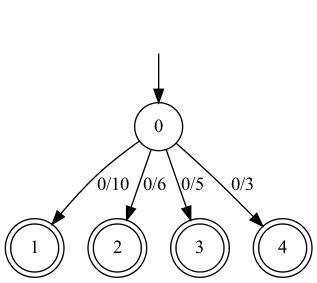
\includegraphics[scale=0.3]{obrazky-figures/add_inners_det_1_img_aut1.png}
        \caption{}
        \label{add_inners_det_1_img_aut1}
    \end{subfigure}
    \hfil
    \begin{subfigure}{.45\textwidth}
        \centering
        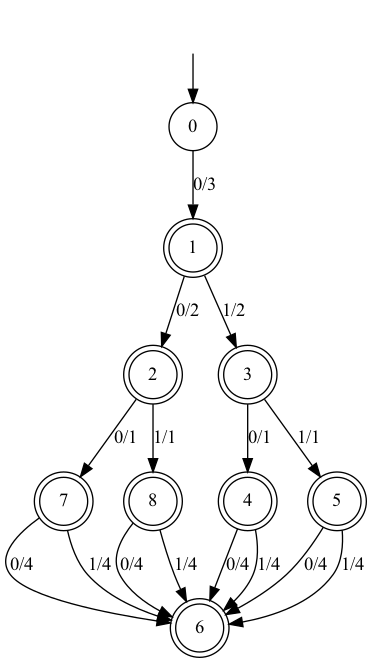
\includegraphics[scale=0.3]{obrazky-figures/add_inners_det_1_img_aut2.png}
        \caption{}
        \label{add_inners_det_1_img_aut2}
    \end{subfigure}
    \hfil
    \begin{subfigure}{.25\textwidth}
        \centering
        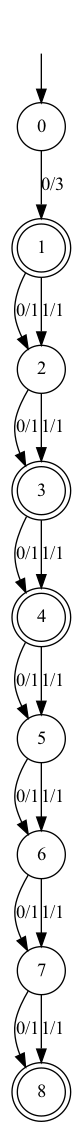
\includegraphics[scale=0.26]{obrazky-figures/add_inners_det_1_img_aut3.png}
        \caption{}
        \label{add_inners_det_1_img_aut3}
    \end{subfigure}
    \caption{Ukázka determinizace automatu z obrázku \ref{add_inners_det_1_img_aut1} pomocí algortimu \ref{add_inners_3}. Obrázek \ref{add_inners_det_1_img_aut2} demonstruje výsledek determinizace za použití metody $add\_trans$ místo $add\_one\_jump\_trans$ na řádcích $12,13$ (což znamená použití maximálních možných délek skip hran) a obrázek \ref{add_inners_det_1_img_aut3} ukazuje výsledný automat přesně dle algoritmu (tedy s přidáváním pouze hran délky $1$ z mezistavů).}
    \label{add_inners_det_1_img}
\end{figure}

\begin{figure}
    \centering
    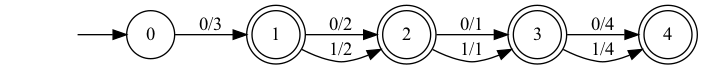
\includegraphics[scale=0.37]{obrazky-figures/add_inners_det_2_img_aut1.png}
    \caption{Ukázka determinizace automatu z obrázku \ref{add_inners_det_1_img_aut1} pomocí algortimu \ref{add_inners_4}.}
    \label{add_inners_det_2_img}
\end{figure}

\paragraph{Algoritmus vytváření mezistavů pro determinizaci (verze 2).} Ve vylepšeném algoritmu \ref{add_inners_4} se opět snažíme zbavit zbytečného větvení pomocí sdílení mezistavů. Myšlenka je taková, že pokud je do nějaké hrany z $s_{a_i}$ do $s_{f_i}$ přidán mezistav $s_{i_i}$, pak se do speciálního vektoru uloží informace o tom, že $s_{i_i}$ je mezistav uvnitř $s_{a_i}$ a $s_{f_i}$. Předveďme si tento přístup na konkrétním příkladu. Nechť existuje automat s dvěma stavy $s_a$ a $s_f$, mezi kterými jsou dvě hrany délky $3$ a $5$ přes symbol $0$ a dvě hrany délky $3$ a $5$ přes symbol $1$. Determinizace započne stavem $s_a$ a symbolem $0$, kde se podívá do speciálního vektoru, jestli existuje mezistav $s_{i_i}$, kde $s_f$ a $s_{f_i}$ jsou tentýž stavy a zároveň hrany $s_{i_i}$ až $s_{f_i}$ a $s_i$ až $s_f$ mají stejnou délku. Takový mezistav zatím neexistuje, vytvoříme tedy nový a uložíme ho do vektoru. Jakmile přijde na řadu zpracování hrany z $s_a$ do $s_f$ přes symbol $1$, tak již podmínka pro nalezení existujícího mezistavu bude splněna a tím pádem se nevytvoří nový mezistav, ale použije se existující. Právě tuto funkcionalitu zajišťuje procedůra $getInnerDet()$. Demonstrace pozitivního efektu této optimalizace je na obrázku \ref{add_inners_det_2_img}.

\begin{algorithm}
    \caption{Vytváření mezistavů během determinizace (verze 2)}
    \label{add_inners_4}
        \begin{algorithmic}[1]
            \Procedure{addInnersDet}{$aut,S_a,S_f,symb$}
                \State $S_{f_{new}} \gets emptyVector()$   
                \State $min\_jump \gets getShortestEdgeLen(S_a,S_f)$
                \For{$s_f$ \textbf{in} $S_f$}
                    \If{$s_f$ has not lowest edge length}
                        \For{$s_a$ \textbf{in} $S_a$}
                            \If{$aut.has\_trans(s_a, symb, s_f)$}
                                \State $aut.remove\_trans(s_a, symb, s_f)$
                                \State $s_i \gets getInnerDet()$
                                \State $aut.add\_trans(s_a,symb,s_i,min\_jump)$
                                \State $S_{f_{new}}.push(s_i)$
                            \EndIf
                        \EndFor
                    \Else
                        \State $S_{f_{new}}.push(s_f)$
                    \EndIf
                \EndFor
                \State $S_f \gets S_{f_{new}}$
            \EndProcedure
        \end{algorithmic}
\end{algorithm} 

\subsection{Komplement}

Komplement pracuje tak, že daný automat zúplní a následně vymění akceptující stavy za neakceptující a obráceně. Toto ovšem pro naši reprezentaci není dostačující, protože skip hrana může přeskočit několik stavů, které nejsou akceptující a tedy tyto stavy se v automatu nevyskytují, což znamená, že v případě potřeby nemohou být změněny na akceptující. Z~toho plyne, že budeme přidávat mezistavy, které budou koncové. Polaritu nemění všechny stavy, ale pouze ty do kterých suma délek hran jdoucích z libovolného počátečního stavu modulo počet proměnných ve formuli je rovna $0$, nebo-li skončit můžeme, když je stejněkrát přiřazeno do všech proměnných. Komplementace je popsána v algoritmu \ref{completement}.

\paragraph{Triviální případy.} Nejprve řešíme triviální případy, které jsou dva. První je pokud máme automat s jedním iniciálním a zároveň akceptujícím stavem a žádné přechody. Toto je detekované podmínkou na řádku $2$, kde $id\_cnt$ je aktuální počet proměnných ve formuli a~metoda $lang\_is\_empty$ vrací $true$, jestliže je jazyk automatu prázdný, jinak $false$. Tuto situaci musíme ošetřit separátně, protože algoritmus by v tomto případě začal tvořit hrany délky $0$, což není povoleno. Druhý speciální případ je, když má vstupní automat prázdný jazyk, což odpovídá podmínce z řádku $5$, pak stačí vrátit automat přijímající všechna přiřazení proměnných. Jak již vyplývá z názvu, funkce $codeTrue$ vyrobí přesně takový automat, naopak procedůra $codeFalse$ vyrobí jednostavový automat bez koncových stavů. 

\begin{algorithm}
    \caption{Komplementace automatu se skip hranami}
    \label{completement}
        \begin{algorithmic}[1]
            \Procedure{complement}{$aut,id\_cnt$}
                \If{$id\_cnt$ = 0 and not $aut.lang\_is\_empty()$}
                    \State \Return $codeFalse()$
                \EndIf
                \If{$aut.lang\_is\_empty()$}
                    \State \Return $codeTrue(id\_cnt)$
                \EndIf
                \State $result \gets emptyAutomaton(aut.num\_states())$
                \State $result.add\_sink\_state()$
                \State $q \gets emptyVector()$
                \State $level \gets emptyArray(aut.num\_states())$
                \State $aut \gets determinization(aut)$ 
                \For{$init$ \textbf{in} $aut.init\_states()$}
                    \State $level[init] \gets 0$
                    \State $result.make\_initial(init)$
                    \State $q.push(init)$
                \EndFor
                \While{$q$ is not empty}
                    \State $s_a \gets q.pop()$
                    \For{$symb, s_f$ \textbf{going from} $s_a$ \textbf{in} $aut$}
                        \State $addFinalStates(result,s_a,symb,s_f,level,id\_cnt)$
                        \If{$s_f$ was not seen}
                            \State $q.push(s_f)$
                        \EndIf
                    \EndFor
                    \If{does not exists $0$ trans from $s_a$}
                        \State $result.add\_trans(s_a,0,s_{sink},id\_cnt-level[s_a])$
                    \EndIf
                    \If{does not exists $1$ trans from $s_a$}
                        \State $result.add\_trans(s_a,1,s_{sink},id\_cnt-level[s_a])$
                    \EndIf
                \EndWhile
                \For{$s_f$ \textbf{in} $aut.final\_states$}
                    \State $result.remove\_final(s_f)$
                \EndFor
                \State \Return $result$
            \EndProcedure
        \end{algorithmic}
\end{algorithm}

\paragraph{Tělo komplementu.} Nyní provedeme determinizaci vstupního automatu, abychom získali vstupní automat s jedním počátečním stavem. Metoda $add\_sink\_state$ vytvoří jeden koncový stav se smyčkou dvou přechodů o délce počtu proměnných přes symboly $0,1$, bežně nazývaný jako \textit{sink stav}. Ještě před hlavním cyklem algoritmu provedeme potřebné inicializace, včetně nastavení pole $level$, jenž slouží k zapamatování si úrovně stavu, kterou definujeme jako součet úrovně libovolného předchůdce daného stavu a délky jejich propojující hrany, to celé modulo počet proměnných ve formuli, nebo-li vzorcem $level[s_f] = (level[s_a] + getEdgeLen(s_a,s_f)) \mod id\_cnt$ s tím, že iniciální stavy mají úroveň $0$. Analogicky můžeme úroveň stavu definovat pomocí následníků a implicitní úrovně $0$ koncových stavů. V hlavním cyklu komplementace poté postupně procházíme hrany (viz podmínka na řádku $20$, která říká vrať všechny hrany reprezentované dvojicemi symbol $symb$ a cílový stav $s_f$, které vedou ze stavu $s_a$ v automatu $aut$), jenž předáme funkci $addFinalStates$. 

\begin{algorithm}[t]
    \caption{Vytvoří nové stavy a nastaví je na koncové}
    \label{add_final_states}
        \begin{algorithmic}[1]
            \Procedure{addFinalStates}{$aut,s_a,symb,s_f,level,id\_cnt$}
                \State $jump \gets getEdgeLen(s_a,s_f)$
                \State $num\_states \gets aut.num\_states()$
                \State $num\_inner\_states \gets \max (0,\lceil \frac{jump + level[s_a] - id\_cnt}{id\_cnt} \rceil)$
                \State $aut.increase\_size(num\_states + num\_inner\_states)$
                \If{$num\_inner\_states = 0$}
                    \State $aut.add\_trans(s_a,symb,s_f,jump)$
                \Else
                    \State $s_{a_{tmp}} \gets s_a$
                    \State $s_{f_{tmp}} \gets num\_states$
                    \State $num\_states \gets num\_states + 1$
                    \State $aut.add\_trans(s_{a_{tmp}},symb,s_{f_{tmp}},id\_cnt-level[s_a])$
                    \For{$i=0$ \textbf{to} $num\_inner\_states-1$}
                        \State $s_{a_{tmp}} \gets s_{f_{tmp}}$
                        \State $s_{f_{tmp}} \gets num\_states$
                        \State $num\_states \gets num\_states + 1$
                        \State $aut.add\_trans(s_{a_{tmp}}, 0, s_{f_{tmp}}, id\_cnt)$
                        \State $aut.add\_trans(s_{a_{tmp}}, 1, s_{f_{tmp}}, id\_cnt)$
                        \State $aut.make\_final(s_{a_{tmp}})$
                    \EndFor
                    \State $s_{a_{tmp}} \gets s_{f_{tmp}}$
                    \State $s_{f_{tmp}} \gets s_f$
                    \State $jump_{tmp} \gets jump - ((num\_inner\_states - 1) * id\_cnt + (id\_cnt - level[s_a]))$
                    \State $aut.add\_trans(s_{a_{tmp}}, 0, s_{f_{tmp}}, jump_{tmp})$
                    \State $aut.add\_trans(s_{a_{tmp}}, 1, s_{f_{tmp}}, jump_{tmp})$
                    \State $aut.make\_final(s_{a_{tmp}})$
                \EndIf
                \State $level[s_f] \gets (level[s_a] + jump) \mod id\_cnt$
                \If{$level[s_f] = 0$}
                    \State $aut.make\_final(s_f)$
                \EndIf
            \EndProcedure
        \end{algorithmic}
\end{algorithm}

\paragraph{Vytváření mezistavů pro komplement.} Procedůra $addFinalStates$ do hrany přidá akceptující mezistavy, pokud tato hrana přeskakuje nějaké stavy s úrovní $0$. Přesněji kolik stavů úrovně $0$ hrana přeskočí, tolik koncových mezistavů přidáme. Zde již plně využíváme pole úrovní stavů, protože k vytváření mezistavů potřebujeme vědět úroveň aktuálního stavu a délku hrany z aktuálního do cílového stavu. V druhé části hlavního cyklu poté realizujeme zúplnění a na závěr ještě ve výsledném automatu změníme stavy odpovídající koncovým, ve vstupním automatu, na nekoncové. Vizualizace této procedůry je na obrázku~\ref{compl_img}.

\begin{figure}[h]
    \centering
    \begin{subfigure}{.38\textwidth}
        \centering
        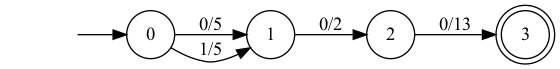
\includegraphics[scale=0.27]{obrazky-figures/compl_img1.png}
        \caption{}
        \label{compl_img1}
    \end{subfigure}
    \hfil
    \begin{subfigure}{.59\textwidth}
        \centering
        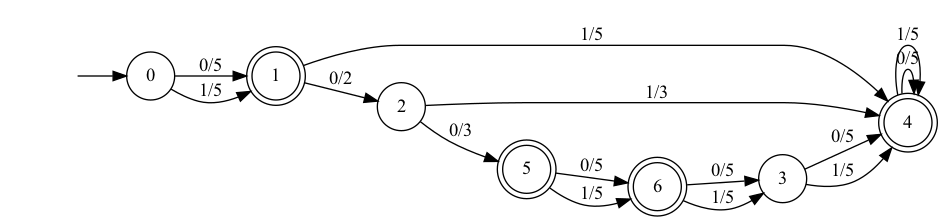
\includegraphics[scale=0.27]{obrazky-figures/compl_img2.png}
        \caption{}
        \label{compl_img2}
    \end{subfigure}
    \caption{Vizualizace činnosti funkce $complement$ pro $5$ proměnných. Na obrázku \ref{compl_img1} vidíme hranu před a na obrázku \ref{compl_img2} po zavolání procedůry. Počáteční stav $0$ slouží pro booleovské proměnné a nenegujeme ho.}
    \label{compl_img}
\end{figure}

\subsection{Projekce}

Jako další automatovou operaci představíme projekci. Myšlenka je taková, že odstraníme určitou proměnnou $x$ z automatu, reprezentovanou jejím indexem $i$, což v terminologii úrovní stavů znamená vymazat všechny přechody ze stavů úrovně $i$ do stavů úrovně $i+1$. V~rámci skip hran mohou během tohoto odstranění nastat tři situace, které rozebereme v~rámci popisu algoritmu. Další obtíž je, že takto získaný automat je obecně nedeterministický, proto v této fázi musí být aplikována determinizace. Následně ještě  nastavíme všechny stavy, ze kterých se lze dostat do libovolného koncového stavu přes symbol $0$, jako koncové. Pseudokód projekce je uveden v algoritmu \ref{project}.

\begin{figure}[h]
    \centering
    \begin{subfigure}{.15\textwidth}
        \centering
        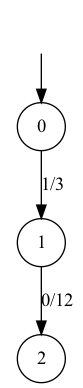
\includegraphics[scale=0.3]{obrazky-figures/proj_img2.png}
        \caption{}
        \label{proj_img2}
    \end{subfigure}
    \hfil
    \begin{subfigure}{.15\textwidth}
        \centering
        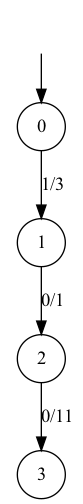
\includegraphics[scale=0.3]{obrazky-figures/proj_img3.png}
        \caption{}
        \label{proj_img3}
    \end{subfigure}
    \hfil
    \begin{subfigure}{.15\textwidth}
        \centering
        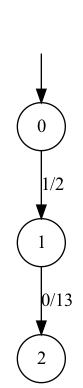
\includegraphics[scale=0.3]{obrazky-figures/proj_img1.png}
        \caption{}
        \label{proj_img1}
    \end{subfigure}
    \hfil
    \begin{subfigure}{.15\textwidth}
        \centering
        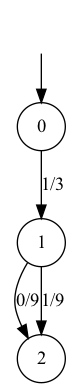
\includegraphics[scale=0.3]{obrazky-figures/proj_img5.png}
        \caption{}
        \label{proj_img5}
    \end{subfigure}
    \hfil
    \begin{subfigure}{.15\textwidth}
        \centering
        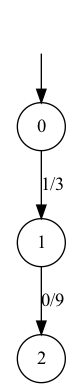
\includegraphics[scale=0.3]{obrazky-figures/proj_img6.png}
        \caption{}
        \label{proj_img6}
    \end{subfigure}
    \hfil
    \begin{subfigure}{.15\textwidth}
        \centering
        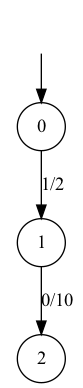
\includegraphics[scale=0.3]{obrazky-figures/proj_img4.png}
        \caption{}
        \label{proj_img4}
    \end{subfigure}
    \caption{Vizualizace projekce proměnné (algoritmus \ref{project}) s indexem $3$ z celkového počtu $5$ti proměnných pro tři různé vstupní automaty. Obrázek \ref{proj_img2} představuje případ podmínky z řádku $24$, jehož výsledný automat je na obrázku \ref{proj_img5}. Analogicky pro dvojice obrázků~\ref{proj_img3},~\ref{proj_img6} (podmínka z řádku $27$) a \ref{proj_img1}, \ref{proj_img4} (případ na řádku $29$).}
    \label{proj_img}
\end{figure}

\paragraph{Triviální případy.} Začínáme opět se dvěma speciálními případy. Jelikož se nemůže stát, že by byla projekce volána s nulovým počtem proměnných ve formuli, budeme řešit případy s jednou proměnnou, a to konkrétně pokud je navíc jazyk vstupního automatu neprázdný, pak vracíme automat s jedním iniciálním a zároveň akceptujícím stavem, jinak vyrobíme automat s jedním iniciálním stavem. 

\begin{algorithm}
    \caption{Nastaví stavy, ze kterých se dá dostat po $0$ do koncového stavu, na koncové}
    \label{removeUselessZeros}
        \begin{algorithmic}[1]
            \Procedure{removeUselessZeros}{$aut,id\_cnt$}
                \State $preds \gets emptyArray(aut.num\_states())$
                \For{$s_a$ \textbf{in} $aut.states$}
                    \For{$symb, s_f$ \textbf{going from} $s_a$ \textbf{in} $aut$}
                        \State $preds[s_f].push((symb,s_a))$
                    \EndFor
                \EndFor
                \State $q \gets emptyVector()$
                \State $level \gets emptyArray(aut.num\_states())$
                \For{$final$ \textbf{in} $aut.final\_states$}
                    \State $level[final] \gets 0$
                    \State $q.push(final)$
                \EndFor
                \While{$q$ is not empty}
                    \State $s_f \gets q.pop()$
                    \For{$p$ \textbf{in} $preds[s_f]$}
                        \State $addFinalStatesRev(aut,p.second,p.first,s_f,level,id\_cnt)$
                        \If{$p.first = 0$ and $p.second$ was not seen}
                            \State $q.push(p.second)$
                        \EndIf
                    \EndFor
                \EndWhile
                \State \Return $aut$
            \EndProcedure
        \end{algorithmic}
\end{algorithm}

\paragraph{Odstranění proměnné.} Na rozdíl od dříve zmíněných algoritmů je zde navíc vektor $edges\_to\_be\_removed$ sloužící k uchovávání dvojic stavů, kde všechny hrany jdoucí do prvního stavu, přesměrujeme do druhého stavu. Zmíněné přesměrování se používá, pokud odstraňujeme hranu délky $1$. Funkce $computeEdgeLen$ zkrátí délku hrany o konstantu, jenž odpovídá počtu uzlů úrovně $i$ přeskočených danou hranou. Následně v hlavním cyklu algoritmu tradičně procházíme všechny hrany, přičemž mohou nastat tři situace (v pseudokódu reprezentováno podmínkami na řádcích $24,27,29$). Úvodní případ znamená, že index $i$ projektované proměnné $x$ je roven úrovni aktuálního stavu a délka hrany je větší než $1$. Intuitivní význam je, že projektovaná proměnná je na začátku skip hrany. Prakticky to znamená, že musíme tuto hranu nahradit dvěma hranami přes symboly $0,1$ s délkami sníženými o počet přeskočených uzlů úrovně $i$ původní hranou. Druhá situace je podobná předchozí, akorát se jedná o běžnou hranu, tedy její délka je $1$. Toto je typická situace vyskytující se i v reprezentaci bez skip hran, takže už budeme muset hranu odstranit a~přesměrovat všechny hrany, směřující do jejího počátečního stavu, do jejího cílového stavu. Na to 

\begin{algorithm}
    \caption{Odstranění proměnné v automatu se skip hranami}
    \label{project}
        \begin{algorithmic}[1]
            \Procedure{project}{$aut,x,id\_cnt$}
                \If{$id\_cnt$ = 1 and not $aut.lang\_is\_empty()$}
                    \State \Return $codeTrue(0)$
                \EndIf
                \If{$id\_cnt$ = 1 and $aut.lang\_is\_empty()$}
                    \State \Return $codeFalse()$
                \EndIf
                \State $result \gets emptyAutomaton(aut.num\_states())$
                \State $result.initial\_states \gets aut.initial\_states$
                \State $result.final\_states \gets aut.final\_states$
                \State $q \gets emptyVector()$
                \State $level \gets emptyArray(aut.num\_states())$
                \State $edges\_to\_be\_removed \gets emptyVector()$
                \For{$init$ \textbf{in} $aut.initial\_states$}
                    \State $level[init] \gets 0$
                    \State $q.push(init)$
                \EndFor
                \While{$q$ is not empty}
                    \State $s_a \gets q.pop()$
                    \For{$symb, s_f$ \textbf{going from} $s_a$ \textbf{in} $aut$}
                        \State $jump \gets getEdgeLen(s_a,s_f)$
                        \State $edge\_len \gets computeEdgeLen(level[s_a], jump, x, id\_cnt)$
                        \State $level[s_f] \gets (level[s_a]+jump) \mod id\_cnt$
                        \If{$level[s_a] = x$ and $jump > 1$}
                            \State $result.add\_trans(s_a, 0, s_f, edge\_len)$
                            \State $result.add\_trans(s_a, 1, s_f, edge\_len)$
                        \ElsIf{$level[s_a] = x$ and $jump = 1$}
                            \State $edges\_to\_be\_removed.push((s_a,s_f))$
                        \Else
                            \State $result.add\_trans(s_a, symb, s_f, edge\_len)$
                        \EndIf
                        \If{$s_f$ was not seen}
                            \State $q.push(s_f)$
                        \EndIf
                    \EndFor
                \EndWhile
                \State $result \gets redirectEdges(result,edges\_to\_be\_removed)$
                \State $result \gets determinize(result)$
                \State $result \gets removeUselessZeros(result, id\_cnt - 1)$
                \State \Return $result$
            \EndProcedure
        \end{algorithmic}
\end{algorithm}

\noindent
použijeme již zmíněný vektor $edges\_to\_be\_removed$. Důvod proč neodstraňujeme hrany teď je, protože iterujeme přes vstupní automat a hrany přidáváme do nového automatu, tím pádem nemáme zaručeno, že jsme již viděli všechny hrany jdoucí do aktuálního stavu a také některé hrany směřující do aktuálního stavu budou později odstraněny a nahrazeny novými, což by se opět neprojevilo ve výsledném automatu. Poslední případ představuje situaci, kdy $i$ a úroveň aktuálního stavu jsou různé. Neformálně řečeno, projektovaná proměnná není na začátku skip hrany. Zde stačí snížit délku hrany o počet přeskočených uzlů úrovně $i$. Tyto tři případy jsou přehledně vizualizovány na obrázku \ref{proj_img}. Poté funkce $redirectEdges$ realizuje podstatu vektoru $edges\_to\_be\_removed$, tedy provede zmíněné přesměrování hran.

\begin{algorithm}[t]
    \caption{Přidání koncových stavů mezi stavy $s_a$ a $s_f$}
    \label{addFinalStatesRev}
        \begin{algorithmic}[1]
            \Procedure{addFinalStatesRev}{$aut,s_a,symb,s_f,level,id\_cnt$}
                \State $jump \gets getEdgeLen(s_a,s_f)$
                \State $num\_states \gets aut.num\_states()$
                \State $num\_inner\_states \gets \max (0,\lceil \frac{jump + level[s_f] - id\_cnt}{id\_cnt} \rceil)$
                \State $aut.increase\_size(num\_states + num\_inner\_states)$
                \If{$num\_inner\_states > 0$}
                    \State $s_{a_{tmp}} \gets num\_states$
                    \State $s_{f_{tmp}} \gets s_f$
                    \State $num\_states \gets num\_states + 1$
                    \State $aut.add\_trans(s_{a_{tmp}},0,s_{f_{tmp}},id\_cnt-level[s_f])$
                    \State $aut.add\_trans(s_{a_{tmp}},1,s_{f_{tmp}},id\_cnt-level[s_f])$
                    \State $aut.make\_final(s_{a_{tmp}})$
                    \For{$i=0$ \textbf{to} $num\_inner\_states-1$}
                        \State $s_{f_{tmp}} \gets s_{a_{tmp}}$
                        \State $s_{a_{tmp}} \gets num\_states$
                        \State $num\_states \gets num\_states + 1$
                        \State $aut.add\_trans(s_{a_{tmp}}, 0, s_{f_{tmp}}, id\_cnt)$
                        \State $aut.add\_trans(s_{a_{tmp}}, 1, s_{f_{tmp}}, id\_cnt)$
                        \State $aut.make\_final(s_{a_{tmp}})$
                    \EndFor
                    \State $s_{f_{tmp}} \gets s_{a_{tmp}}$
                    \State $s_{a_{tmp}} \gets s_a$
                    \State $jump_{tmp} \gets jump - ((num\_inner\_states - 1) * id\_cnt + (id\_cnt - level[s_f]))$
                    \State $aut.add\_trans(s_{a_{tmp}}, symb, s_{f_{tmp}}, jump_{tmp})$
                    \State $aut.remove\_trans(s_a, symb, s_f)$
                \EndIf
                \State $level[s_a] \gets (level[s_f] + jump) \mod id\_cnt$
                \If{$level[s_a] = 0$ and $symb = 0$ and $s_a$ is not initial}
                    \State $aut.make\_final(s_a)$
                \EndIf
            \EndProcedure
        \end{algorithmic}
\end{algorithm}

\paragraph{Odstranění zbytečných nul.} V neposlední řadě ještě procedůrou $removeUselessZeros$ nastavíme všechny stavy ze kterých se lze dostat do koncových stavů pomocí libovolného počtu přechodových symbolů $0$, jako koncové. Ta je implementována tak, že nejprve do pole $preds$ vypočte všechny předchůdce všech stavů spolu s příslušnými přechodovými symboly a následně zpětně iteruje automatem, tedy směrem z koncových do počátečních stavů a všechny hrany jdoucí z předchůdců do aktuálního stavu rozmělní mezistavy, podobně jako při komplementaci. Tato optimalizace slouží k tomu, abychom nemuseli několikrát prohledávat celý automat při hledání předchozích stavů, ale pouze jedenkrát. Procedůra $addFinalStatesRev$ realizuje zmiňované přidání mezistavů obdobným způsobem jako $addFinalStates$ v algoritmu \ref{completement}, akorát v opačném směru.

\subsection{Minimalizace}

Jako minimalizační algoritmus jsme zvolili Brzozowski algoritmus doplněný o redukci běžných hran na skip hrany, a to z důvodu, že se již nachází v námi používané knihovně Mata a patří mezi používané, ovšem může u něj dojít ke stavové explozi. Jedná se o dvojitou reverzaci následovanou determinizací, což je formálněji vyjádřeno algoritmem \ref{minimization}.

\begin{algorithm}[h]
    \caption{Minimalizace vstupního automatu}
    \label{minimization}
        \begin{algorithmic}[1]
            \Procedure{minimization}{$aut$}
                \State $aut = revert(aut)$
                \State $aut = determinization(aut)$
                \State $aut = revert(aut)$
                \State $aut = determinization(aut)$
                \State $aut = reduceToSkipEdges(aut)$
                \State \Return $aut$
            \EndProcedure
        \end{algorithmic}
\end{algorithm}

\begin{figure}[h]
    \centering
    \begin{subfigure}{.2\textwidth}
        \centering
        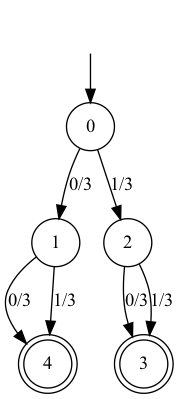
\includegraphics[scale=0.3]{obrazky-figures/revert_img1.png}
        \caption{}
        \label{revert_img1}
    \end{subfigure}
    \hfil
    \begin{subfigure}{.4\textwidth}
        \centering
        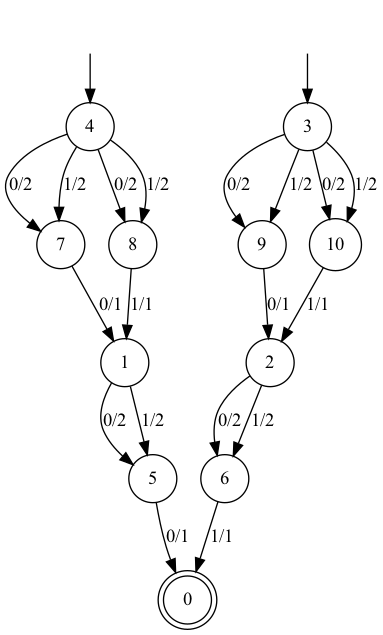
\includegraphics[scale=0.3]{obrazky-figures/revert_img2.png}
        \caption{}
        \label{revert_img2}
    \end{subfigure}
    \hfil
    \begin{subfigure}{.3\textwidth}
        \centering
        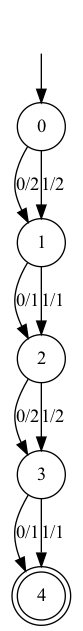
\includegraphics[scale=0.3]{obrazky-figures/revert_img3.png}
        \caption{}
        \label{revert_img3}
    \end{subfigure}
    \caption{Vizualizace průběhu reverzace automatu \ref{revert_img1}, kde na obrázku \ref{revert_img2} je reverzovaný s přidanými nesdílenými mezistavy $5,6,7,8,9,10$ a následně determinizovaný na obrázku \ref{revert_img3}. Množiny stavů během determinizace byly $\{3,4\}$, $\{7,8,9,10\}$, $\{1,2\}$, $\{5,6\}$, $\{0\}$, kde počet uvedených množin by zůstal stejný i při použití sdílených mezistavů, tedy determinizace by trvala stejný počet kroků.}
    \label{revert_img}
\end{figure}

\paragraph{Reverzace.} Funkce $revert$ (algoritmus \ref{revert}), jak již název napovídá, provede reverzaci automatu. Pro hrany délky $1$ je algoritmus totožný s klasickou reverzací, jinak se od běžné reverzace lišíme tím, že pro hranu délky $n$ jdoucí ze stavu $s_a$ do $s_f$ přes symbol $symb$ vytvoříme mezistav $s_i$ a nahradíme ji hranami přes oba symboly $0,1$ z $s_f$ do $s_i$ délky $n-1$ a hranou z $s_i$ do $s_a$ přes symbol $symb$ o délce $1$. Díky tomu, že po reverzaci přijde vždy determinizace, tak není nutné sdílet mezistavy (např. jako v algoritmech \ref{add_inners_2} a \ref{add_inners_4} pro průnik či determinizaci), protože determinizace sjednotí nesdílené mezistavy do jednoho stejným způsobem, jako kdyby byl sdílený, což můžeme vidět na obrázku \ref{revert_img}.

\begin{algorithm} % TODO zkonstrolovat u vsech algo ze kdyz u add_trans neni 4. parametr tak je delka hrany=1
    \caption{Reverzace vstupního automatu}
    \label{revert}
        \begin{algorithmic}[1]
            \Procedure{revert}{$aut$}
                \State $result \gets emptyAutomaton(aut.num\_states())$
                \State $result.initial\_states \gets aut.final\_states$
                \State $result.final\_states \gets aut.initial\_states$
                \For{$s_a$ \textbf{in} $aut.states$}
                    \For{$symb, s_f$ \textbf{going from} $s_a$ \textbf{in} $aut$}
                        \State $jump \gets getEdgeLen(s_a,s_f)$
                        \If{$jump = 1$}
                            \State $result.add\_trans(s_f,symb,s_a)$
                        \Else
                            \State $s_i \gets result.add\_state()$
                            \State $result.add\_trans(s_f,0,s_i,jump-1)$
                            \State $result.add\_trans(s_f,1,s_i,jump-1)$
                            \State $result.add\_trans(s_i,symb,s_a)$
                        \EndIf
                    \EndFor
                \EndFor
                \State \Return $result$
            \EndProcedure
        \end{algorithmic}
\end{algorithm}

\paragraph{Redukce na skip hrany.} Hlavní odlišnost oproti běžné minimalizaci je použití funkce $reduceToSkipEdges$, popsané algoritmem \ref{reduceToSkipEdges}. Hlavní myšlenka této procedůry je nahradit hrany v automatu za skip hrany s co nejvetší možnou délkou a díky tomu snížit celkový počet stavů. Na začátku si pomocí funkce $getPredCount$ spočítáme počet předcházejících stavů pro každý stav. Poté iterujeme skrz hrany automatu a voláme na ně funkci $addSkipEdge$, která danou hranu prodlouží na maximální možnou délku. Tato procedůra je vytvořená pouze pro deterministické konečné automaty, což nevadí protože redukce na skip hrany je aplikována právě po determinizaci. Nicméně vytvořili jsme také nedeterministickou verzi ekvivalentního algoritmu s vidinou toho, že bychom ji aplikovali mezi reverzací a determinizací, ale ta se prokázala jako neefektivní. Funkce $addSkipEdge$ (algoritmus \ref{addSkipEdge}) funguje tak, že v nekonečném cyklu máme první ukončující podmínku říkající, že nově vytvořená skip hrana se už nemůže dále prodloužit, pokud z aktuálního stavu již žádná hrana nevede nebo je koncový (koncový stav nelze přeskočit, protože bychom o něj přišli) nebo už je v~aktuálně zpracovávané hraně obsažen. Dále funkce $getNextState$ vrací libovolný stav do kterého vede hrana ze stavu uvedeného jako parametr. Druhá podmínka zní, že z aktuálního stavu do takto získaného musí vést přechody přes oba symboly $0,1$ a aktuální stav má méně než $2$ předchůdce. Pokud není splněna, pak výroba hrany končí. V tomto okamžiku

\begin{algorithm}
    \caption{Nahradí všechny hrany za co nejdelší skip hrany}
    \label{reduceToSkipEdges}
        \begin{algorithmic}[1]
            \Procedure{reduceToSkipEdges}{$aut$}
                \State $result \gets emptyAutomaton(aut.num\_states())$
                \State $result.initial\_states \gets aut.initial\_states$
                \State $result.final\_states \gets aut.final\_states$
                \State $q \gets emptyVector()$
                \State $pred \gets getPredCount(aut)$
                \For{$init$ \textbf{in} $aut.initial\_states$}
                    \State $q.push(init)$
                \EndFor
                \While{$q$ is not empty}
                    \State $s_a \gets q.pop()$
                    \For{$symb, s_{f_{tmp}}$ \textbf{going from} $s_a$ \textbf{in} $aut$}
                        \State $jump \gets getEdgeLen(s_a,s_{f_{tmp}})$
                        \State $s_f,jump \gets addSkipEdge(aut, s_{f_{tmp}}, jump, pred)$
                        \State $result.add\_trans(s_a, symb, s_f, jump)$
                        \If{$s_f$ was not seen}
                            \State $q.push(s_f)$
                        \EndIf
                    \EndFor
                \EndWhile
                \State \Return $result$
            \EndProcedure
        \end{algorithmic}
\end{algorithm}

\begin{algorithm}
    \caption{Vypočítá délku skip hrany a cílový stav}
    \label{addSkipEdge}
        \begin{algorithmic}[1]
            \Procedure{addSkipEdge}{$aut,init\_state,init\_jump,pred$}
                \State $edge\_len \gets init\_jump$
                \State $s_a \gets init\_state$
                \While{true}
                    \If{does not exists trans from $s_a$ or $s_a$ is final or $s_a$ was seen}
                        \State \Return $s_a$, $edge\_len$
                    \EndIf
                    \State $s_f \gets getNextState(s_a)$
                    \If{$aut.has\_trans(s_a,0,s_f)$ and $aut.has\_trans(s_a,1,s_f)$ and $pred[s_a] < 2$}
                        \State $s_a \gets s_f$
                        \State $jump \gets getEdgeLen(s_a,s_f)$
                        \State $edge\_len \gets edge\_len + jump$
                    \Else
                        \State \Return $s_a$, $edge\_len$
                    \EndIf
                \EndWhile
            \EndProcedure
        \end{algorithmic}
\end{algorithm}

\noindent
máme hotový algoritmus, jenž vyrobí maximálně dlouhé skip hrany mezi všemi dvojicemi stavů s méně než dvěma předchůdci, což na první pohled zní uspokojivě, ale po bližším zkoumání jsme zjistili, že při rozvolnění podmínky o počtu předchůdců (část $pred[s_a]<2$ na řádku $9$ v algoritmu \ref{addSkipEdge}) budou sice některé skip hrany delší o příslušnou konstantu odpovídající délce společné cesty v původním automatu, ale získáme menší celkový počet stavů. Z těchto důvodů jsme se rozhodli dále používat druhý přístup (bez podmínky na předchůdce stavů). Porovnání obou přístupů k redukci na skip hrany můžeme vidět na obrázku \ref{reduce_img}.

\begin{figure}[h]
    \centering
    \begin{subfigure}{.99\textwidth}
        \centering
        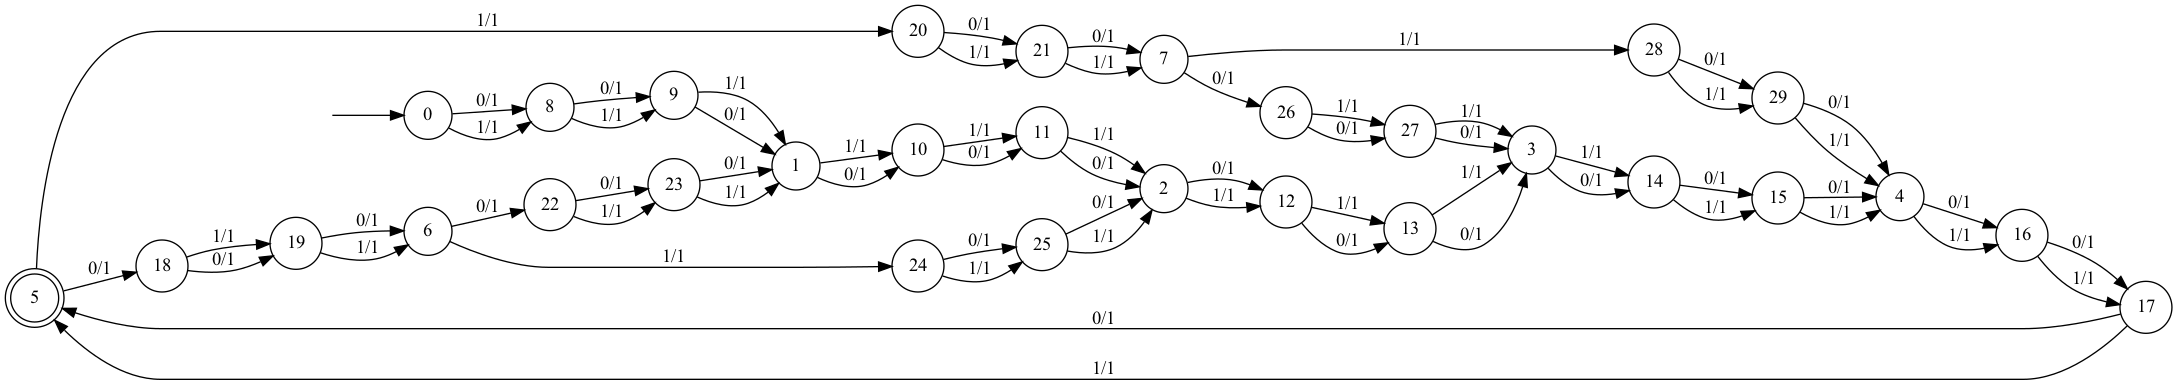
\includegraphics[scale=0.19]{obrazky-figures/reduce_img1.png}
        \caption{}
        \label{reduce_img1}
    \end{subfigure}
    \vfil
    \begin{subfigure}{.99\textwidth}
        \centering 
        \begin{subfigure}{.6\textwidth}
            \centering
            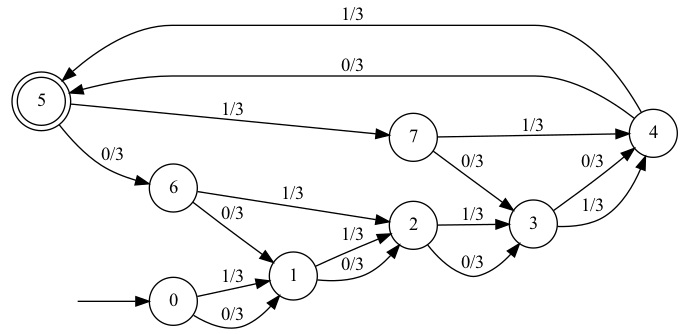
\includegraphics[scale=0.22]{obrazky-figures/reduce_img2.png}
            \caption{}
            \label{reduce_img2}
        \end{subfigure}
        \hfil
        \begin{subfigure}{.35\textwidth}
            \centering
            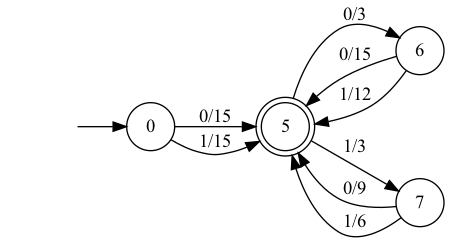
\includegraphics[scale=0.28]{obrazky-figures/reduce_img3.png}
            \caption{}
            \label{reduce_img3}
        \end{subfigure}
    \end{subfigure} 
    \caption{Demonstrace redukce na skip hrany automatu z obrázku \ref{reduce_img1}. Na obrázku \ref{reduce_img2} je verze algoritmu s podmínkou na počet předchůdců a na obrázku \ref{reduce_img3} je verze bez této podmínky.}
    \label{reduce_img}
\end{figure}

\chapter{Implementace}
\label{3_implementace}

V naší implementaci používáme překladač formulí a abstraktní syntaktický strom z nástroje Mona (zdrojové soubory z \texttt{/src/ast} a \texttt{/include}), kam jsme přidali funkce pro výrobu automatů. Pro práci s konečnými automaty jsme využili knihovnu Mata\footnote{https://github.com/VeriFIT/mata} (zdrojové soubory z \texttt{/src/mata} a \texttt{/include}), do které jsme přidali implementaci skip hran a upravili tradiční automatové algoritmy pro efektivní práci s naší reprezentací. V adresáři \texttt{/src/core} jsou naše vlastní zdrojové kódy pro řízení transformace formule na automat, zbylé automatové operace a statistiky.

\section{Mata reprezentace automatů}

Předtím než popíšeme implementaci složitějších součástí, rozebereme jak vypadá reprezentace konečného automatu v knihovně Mata. Přechodová relace je vektor obsahující \textit{Moves} o délce počtu stavů automatu, kde každý index $i$ obsahuje přechody automatu ze stavu $i$, což je označno jako Moves. Moves je poté vektor složený z \textit{Move}, který je seřazený podle přechodového symbolu a každá jeho položka představuje přechod přes právě jeden symbol. Konečně, Move je struktura obsahující přechodový symbol (nezáporné číslo) a vektor cílových stavů, opět seřazený. Vidíme, že zmíněná datová struktura je vytvořena obecně pro nedeterministické konečné automaty. Počátěční a koncové stavy jsou navíc ještě uloženy v~samostatných dvou vektorech. Grafická ukázka je na obrázku \ref{mata_aut}.

\begin{figure}[ht]
    \begin{subfigure}{.45\textwidth}
        \centering
        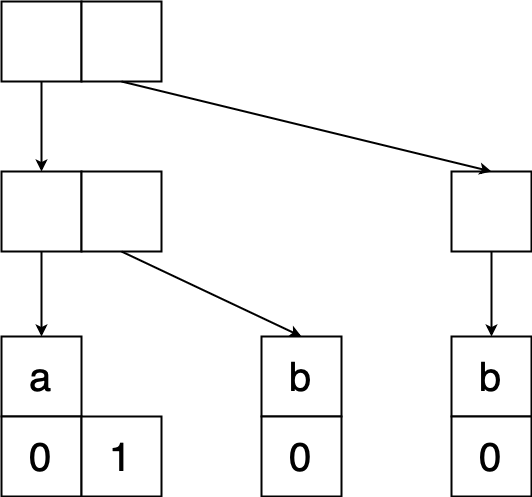
\includegraphics[scale=0.25]{obrazky-figures/mata_aut.png}
        \caption{Mata reprezentace automatu.}
        \label{mata_aut_tr}
    \end{subfigure}%
    \hfil
    \begin{subfigure}{.45\textwidth}
        \centering
        \begin{tikzpicture}[shorten >=1pt,node distance=2cm,on grid,auto] 
            \node[state] (Q_0)  {$0$}; 
            \node[state,] (Q_1) [right=of Q_0] {$1$};
            \path[->]
                (Q_0) edge [bend left] node {$a$} (Q_1)
                edge [loop above] node {$a$} ()
                edge [loop below] node {$b$} ()
                (Q_1) edge [bend left] node {$b$} (Q_0);
        \end{tikzpicture}
        \caption{Konečný automat.}
        \label{mata_aut_aut}
    \end{subfigure}
    \caption{Vizualizace datové struktury konečného automatu v knihovně Mata. Jako symboly jsou z důvodu přehlednosti zvolena písmena $a,b$, ovšem reálně mohou symboly být pouze nezáporná čísla.}
    \label{mata_aut}
\end{figure}

\section{Skip hrany}

Datovou strukturu konečného automatu jsme upravili tak, že vektor cílových stavů již neobsahuje cílové stavy, ale obsahuje dvojice cílový stav a délka hrany. Tento přístup odpovídá přidání informace o přeskakování ke hranám. Další možnost byla přiřadit tuto informaci, modulovanou, ke stavům a dát jim úroveň, pak bychom ale dostali chování totožné s BDD, tedy maximální délka hrany by odpovídala počtu proměnných, protože pokud bychom měli přechod z úrovně $0$ do úrovně $2$, tak nevíme jestli je délka této hrany $2$ nebo počet proměnných $+2$. Jestliže bychom chtěli úroveň udělat nemodulovanou, narazíme na to, že pokud bude na nějakém stavu smyčka, tak by jeho úroveň byla nekonstantní. Ukázka datové struktury pro jednoduchý automat je na obrázku \ref{mata_skip_aut}.

\begin{figure}[ht]
    \begin{subfigure}{.45\textwidth}
        \centering
        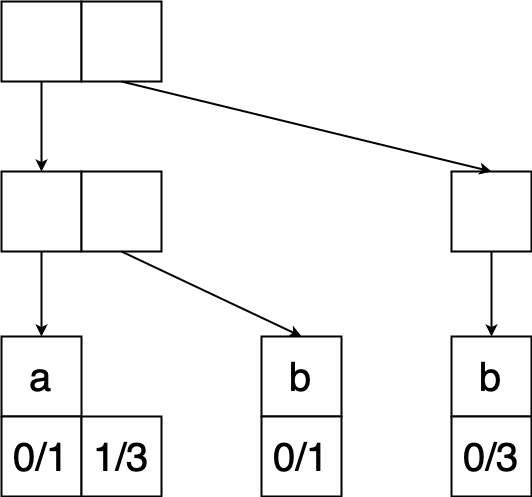
\includegraphics[scale=0.25]{obrazky-figures/mata_skip_aut.png}
        \caption{Mata reprezentace automatu obohacená o skip hrany.}
        \label{mata_skip_aut_tr}
    \end{subfigure}%
    \hfil
    \begin{subfigure}{.45\textwidth}
        \centering
        \begin{tikzpicture}[shorten >=1pt,node distance=2cm,on grid,auto] 
            \node[state] (Q_0)  {$0$}; 
            \node[state,] (Q_1) [right=of Q_0] {$1$};
            \path[->]
                (Q_0) edge [bend left] node {$a/3$} (Q_1)
                edge [loop above] node {$a/1$} ()
                edge [loop below] node {$b/1$} ()
                (Q_1) edge [bend left] node {$b/3$} (Q_0);
        \end{tikzpicture}
        \caption{Konečný automat se skip hranami.}
        \label{mata_skip_aut_aut}
    \end{subfigure}
    \caption{Ilustrace konečného automatu se skip hranami a jeho implementace s využitím automatové knihovny Mata. V této knihovně mohou být symboly pouze nezáporná čísla, ale pro větší přehlednost jsou na obrázku zvolena písmena $a,b$.}
    \label{mata_skip_aut}
\end{figure}

\section{Kostra převodu formule na automat}

Z nástroje Mona jsme převzali překladač formulí, tabulku predikátů, tabulku symbolů a~abstraktní syntaktický strom. Tím pádem WS1S formule na vstupu našeho programu má identickou syntax jako v nástroji Mona. Výpočet formule probíhá tedy klasicky, a to od atomických formulí směrem k hlavní formuli. Pro zvýšení efektivity jsme se rozhodli v každém kontextu uvažovat pouze proměnné, které jsou relevantní. Například formule $ (\exists y: y = x) \wedge (\exists z: z = x) $ obsahuje celkově tři proměnné $x,y,z$, ale v části vlevo od konjunkce lze uvažovat pouze $x,y$, podobně ve zbylé části $x,z$. V tabulce symbolů se proměnným přiřazuje nezáporné číslo, označované jako \textit{id}. Nejprve se přiřadí globálním proměnným (proměnné zadefinované na začátku programu) a poté proměnným vzniklým kvantifikací ($\exists, \forall$), oběma vzestupně dle výskytu ve formuli. Ve výše uvedené formuli by \textit{id} vypadala následovně: $ (\exists 1: 1 = 0) \wedge (\exists 2: 2 = 0) $. Toto může vyústit v problémy, protože v pravé části formule máme dvě proměnné $x,z$, ale \textit{id} jedné z nich je vyšší než celkový počet proměnných, proto jsme se rozhodli proměnné přemapovávat. Vždy při kvantifikaci přiřadíme nově vzniklým proměnným \textit{id}, které bude rovno aktuálnímu počtu proměnných v daném kontextu, nebo-li bude o $1$ vyšší než aktuální nejvyšší \textit{id} proměnné. Toto mapování, implementované třídou \textit{remapVars}, bude procházet napříč generováním formule a~sbírat potřebná přemapování. Seznam přemapování se využije když narazíme na použití proměnných v nějaké podformuli, a to tak, že v podformuli nahradíme reálné \textit{id} proměnné za přemapované.

\section{Popis průchodu formulí}

Samotná transformace formule na automat se skládá z jednoho průchodu abstraktním syntaktickým stromem, reprezentovaným třídou \textit{AST} a třídami dědícími z \textit{AST}, které představují už jednotlivé termy z WS1S. Každá takováto třída pak obsahuje metodu \textit{genCode}, která bere jako parametry aktuální počet proměnných, seznam přemapování, proměnnou určenou ke sdílení informace a následně z daného termu vytvoří automat. Průchod abstraktním syntaktickým stromem je rozdělen na dvě fáze, zanoření (směr z hlavní formule do atomických formulí) a vynoření (směr z atomických formulí do hlavní formule). Pro další vysvětlení potřebujeme termy rozřadit do šesti kategorií:

\begin{itemize}
    \item Termy nultého (formule) řádu s argumenty nultého řádu bez kvantifikování (např. $\wedge,\neg$)
    \item Kvantifikování s argumenty nultého (formule) řádu (např. $\exists,\forall$)
    \item Proměnné (např. $x$)
    \item Termy nultého (formule) řádu s argumenty prvního (čísla) a druhého (množiny) řádu (např. $<,\subseteq,\in$)
    \item Termy prvního (čísla) a druhého (množiny) řádu (např. $+,\cup$)
    \item Predikáty (např. $xor(x,y) = (x \wedge \neg y) \vee (\neg x \wedge y$))
\end{itemize}

\paragraph{Termy nultého řádu s argumenty nultého řádu bez kvantifikování.} Zde je situace velmi jednoduchá, stačí pouze zavolat tvorbu automatů pro všechny argumenty s~nezměněnými parametry a poté provést příslušnou automatovou operaci.

% TODO popsat treba ze and se neminimaliizuje a tak, popr vytvorit samotatne tema pro minimalizaci

\paragraph{Kvantifikování s argumenty nultého řádu.} Jak již bylo popsáno, v naší implementaci je potřeba měnit \textit{id} proměnných podle aktuálního kontextu. Pro tento učel byla vytvořena třída \textit{remapVars}, což je vektor tvořený z \textit{id} proměnných, kde na $i$-té pozici je původní \textit{id} proměnné a na $i+1$-té pozici je nově vzniklé \textit{id}. V tomto případě nám vznikají proměnné, které dosud nebyly uvažovány, tím pádem při zanoření vytvoříme všem novým proměnným přemapování takové, že první kvantifikovaná proměnná bude namapována na hodnotu aktuálního počtu proměnných, druhá na aktuální počet proměnných $+1$ a analogicky zbytek. Dále zvýšíme aktuální počet proměnných o počet kvantifikovaných proměnných a spolu s~aktualizovaným přemapováním zavoláme funkci na generování automatu z formule, která následuje. V rámci vynoření pak kvantifikované proměnné odprojektujeme, ovšem pokud se jedná o univerzální kvantifikaci, pak zkomplementujeme automat vzniklý z dané formule, odprojektujeme proměnné a nakonec znovu aplikujeme komplement. Další omezení nastává u prvořádových proměnných, kdy před každou projekcí je konjunkcí přidán singleton automat. 

\paragraph{Proměnné.} Tento případ je triviální, ale dá se na něm demonstrovat využití přemapování proměnných. Pokud při průchodu abstraktního syntaktického stromu dojdeme na nejnižší úroveň, tedy k samotné proměnné, přistoupíme k jejímu \textit{id}, ovšem nyní musíme projít seznam přemapování, abychom následně dostali správné \textit{id} vzhledem k aktuálnímu kontextu. U proměnných nultého řádu pouze zavoláme funkci na tvorbu atomického automatu pro přemapovanou proměnnou, u prvního a druhého řádu zavoláme procedůru na rovnost přemapované proměnné a proměnné pro sdílení informace. To je z důvodu, že je nelze chápat jako samostatné formule, ale jejich výskyt je vždy ve formulích s argumenty těchto řádů, pro které proměnnou pro sdílení informace využíváme.

\paragraph{Termy nultého řádu s argumenty prvního a druhého řádu.} Při zanoření se na oba dva argumenty zavolá metoda \textit{getDepth}, která spočítá hloubku zanoření pro obě strany formule, nebo-li kolik pomocných proměnných je potřeba vytvořit. Problematiku uvedeme na příkladu. Nechť máme formuli s argumenty prvního řádu $x+1+2=y+2$. Levá strana formule se převede do tvaru $ x_0 = x_1 + 1 \wedge x_1 = x_2 + 2 \wedge x_2 = x $, pravá obdobně na $ y_0 = y_1 + 2 \wedge y_1 = y $. Metoda \textit{getDepth} tedy v tomto konkrétním případu spočítá, že je potřeba vytvořit $3$ pomocné proměnné pro levou stranu a $2$ pro stranu pravou. Je nutné tento krok udělat nyní, protože zmíněné hodnoty potřebujeme vědět pro výpočet obou stran formule. Následně se zavolá tvorba automatu pro levou stranu formule s tím, že se nastaví proměnná pro sdílení informace na aktuální počet proměnných, tedy $2$, což představuje proměnnou $x_0$. Analogicky pro pravou část, ovšem proměnná pro sdílení informace bude rovna aktuálnímu počtu proměnných zvětšenému o počet pomocných proměnných levé strany, tedy $2+3=5$, a~to značí proměnnou $y_0$. K těmto voláním ještě přiřadíme nový aktuální počet proměnných, který se vypočítá přičtením počtu pomocných proměnných k současnému, který činí $2$, tedy výsledek bude $2+2+3=7$. Až se vynoříme, vytvoříme atomický automat pro rovnost proměnných $x_0$ a $y_0$, zprůnikujeme ho s výslednými automaty pro obě strany a~odprojektujeme všechny pomocné proměnné $x_0,x_1,x_2,y_0,y_1$.

\paragraph{Termy prvního a druhého řádu.} Ve fázi zanoření se podíváme na proměnnou pro sdílení informace, označme ji jako $x$ a vytvoříme další proměnnou $y$ s \textit{id} o $1$ větším než $x$. Nyní zavoláme tvorbu automatu pro argument termu (např. další vnořené $+,-$) s tím, že proměnnou pro sdílení informace nastavíme na $y$. Při vynoření uděláme průnik získaného automatu s daným atomickým automatem (např. $+,-$) pro $x$ a $y$.

\paragraph{Predikáty.} Predikáty jsou v nástroji Mona způsoby jak parametrizovat a znovupoužívat formule. Jako parametr, kromě proměnné, může figurovat libovolný term řádu odpovídajícímu definici predikátu. Například, pokud predikát $foo$ má jeden prvořádový parametr, lze ho volat třeba jako $foo(x)$ i $foo(x + 2)$. Tvorba predikátů je často využívána a z toho důvodu je podporována i v našem nástroji. Způsob výpočtu budeme ilustrovat na příkladu s predikátem $multi\_eq(x,y,z) = x = y \wedge y = z$ a formulí $multi\_eq(a,b,b+1)$. Nejprve při zanoření potřebujeme určit, zda je potřeba vytvářet pomocné proměnné. Iterujeme tedy přes parametry volání a pokud je parametr jen proměnná, není třeba vytvářet pomocnou a stačí ji jen přemapovat, stejně jako když se v běžné formuli narazí na proměnnou, jinak musíme vytvořit pomocnou proměnnou. Nyní budeme požadovat, aby kdykoliv, kdy narazíme v predikátu na proměnnou z jeho definice, tak aby se přemapovala na proměnnou z volání či pomocnou proměnnou, tedy ještě takové přemapování přidáme. Uvedená formule, okleštěná o volání predikátu, bude vypadat takto: $a = b \wedge b = x_0$, kde $x_0$ je vytvořená pomocná proměnná. Dále zavoláme funkci na tvorbu automatu pro výše uvedenou formuli. Během fáze vynoření musíme všechny pomocné proměnné položit rovno jejím volaným parametrům, tedy v tomto příkladu by se nám formule rozrostla o jednu konjunkci: $a = b \wedge b = x_0 \wedge x_0 = b + 1$. Konečně, jestě musíme všechny pomocné proměnné prvního řádu konjunktovat se singleton automatem a úplně všechny pomocné proměnné odprojektovat.

%\section{Atomické automaty} % TODO smazat nebo nechat

%Během výpočtu hlavní formule je nutné v určitých okamžicích vytvářet automaty pro operace WS1S logiky, jako jsou $0,+,-,\emptyset,\cup,\cap,\setminus,\{ \dots \},<,\leq,=,\neq,\subseteq,\in,\notin$. Za tímto účelem jsme vytvořili funkce, které jsou parametrizované speciálně zakódovanou přechodovou relací a slouží ke tvorbě libovolných automatů s jednou, dvěma a třemi proměnnými.

\chapter{Experimenty}
\label{4_experimenty}

Pro otestování naší rozhodovací procedůry a změření její efektivity jsme použili testovací množinu čítající 196 WS1S formulí, rozdělených do následujících 11 kategorií: basic (104), horn-sub (6), horn-trans (6), presburger (10), set-closed (3), set-sing (3), strand (26), strand-adv (13), toss (3), unground (8) a veanes (14). V rámci vyhodnocování jsme se rozhodli použít metriky času a počtu stavů, což je detailně popsáno v tabulkách \ref{exp1_tbl1} a \ref{exp1_tbl2}, kde tabulka~\ref{exp1_tbl1} ukazuje výsledky evaluace pro náš  algoritmus a tabulka \ref{exp1_tbl2} prezentuje ekvivalentní vyhodnocení z nástroje Mona. Časové výsledky vizualizované bodovým diagramem jsou na obrázku \ref{exp_scatter1}. Abychom získali časové a stavové porovnání na stejném počtu formulí, tak tato sada obsahuje pouze formule vypočetlé oběma algoritmy bez dovršení časového stropu. Formule, které byly terminovány jsou z $5$-ti kategorií, jmenovitě horn-sub,

\begin{table}[h]
    \centering
    \begin{tabular}{ |c||c|c|c|c||c|c|c|c||c| } 
        \hline
         & $i_{\wedge}$ & $\Sigma_{\wedge}$ & $\Sigma_{\wedge} / i_{\wedge}$ & $\max_{\wedge}$ & $i_{\exists}$ & $\Sigma_{\exists}$ & $\Sigma_{\exists} / i_{\exists}$ & $\max_{\exists}$ & $t[ms]$ \\ 
        \hline\hline
        basic & 837 & 7557 & 9,029 & 1571 & 629 & 4646 & 7,386 & 1065 & 2874 \\
        \hline
        horn-sub & 105 & 1932 & 18,4 & 773 & 111 & 867 & 7,811 & 450 & 10280 \\ 
        \hline
        horn-trans & 6147 & 43001 & 6,995 & 60 & 4635 & 24177 & 5,216 & 42 & 14750 \\
        \hline
        presburger & 490 & 5765 & 11,765 & 282 & 310 & 2626 & 8,471 & 199 & 2230 \\ 
        \hline
        set-closed & 93 & 1952 & 20,989 & 245 & 72 & 854 & 11,861 & 176 & 958 \\
        \hline
        set-sing & 54 & 1043 & 19,315 & 170 & 45 & 480 & 10,667 & 143 & 1753 \\
        \hline
        strand & 1340 & 19454 & 14,518 & 1006 & 976 & 9118 & 9,342 & 546 & 4395 \\
        \hline
        strand-adv & 1579 & 87421 & 55,365 & 15029 & 1140 & 21739 & 19,069 & 6833 & 9257 \\
        \hline
        toss & 39 & 1473 & 37,769 & 506 & 33 & 348 & 10,545 & 153 & 990 \\
        \hline
        unground & 80 & 921 & 11,512 & 178 & 40 & 414 & 10,35 & 118 & 236 \\
        \hline
        veanes & 178 & 2495 & 14,017 & 365 & 123 & 1159 & 9,423 & 245 & 593 \\ 
        \hline\hline
        $\Sigma$ & 10942 & 173014 & 219,674 & 20185 & 8114 & 66428 & 110,141 & 9970 & 48316 \\
        \hline
    \end{tabular}
    \caption{Výsledky experimentů z našeho algoritmu. Řádky odpovídají sumě meřené vlastnosti, definované sloupcem (např. $i_{\wedge}$), jednotlivých formulí z kategorie označené daným řádkem (např. basic). Poslední řádek (značen $\Sigma$) představuje součet daného sloupce. Symboly ve sloupcích znamenají následující, $i_{\alpha}$ označuje počet volání operace $\alpha$, $\Sigma_{\alpha}$ značí sumu počtu stavů automatu po provedení operace $\alpha$, $\Sigma_{\alpha} / i_{\alpha}$ označuje podíl přechozích dvou hodnot, tedy průměrný počet stavů automatu po dokončení operace $\alpha$ a $\max_{\alpha}$ značí sumu maximálních velikostí automatů v jednotlivých formulích z příslušné kategorie po provedení operace $\alpha$, kde $\alpha$ je buď operace průniku ($\wedge$) nebo projekce ($\exists$). Poslední sloupec ($t[ms]$) představuje dobu trvání výpočtu všech formulí z dané kategorie v milisekundách.}
    \label{exp1_tbl1}
\end{table}

\begin{table}
    \centering
    \begin{tabular}{ |c||c|c|c|c||c|c|c|c||c| } 
        \hline
         & $i_{\wedge}$ & $\Sigma_{\wedge}$ & $\Sigma_{\wedge} / i_{\wedge}$ & $\max_{\wedge}$ & $i_{\exists}$ & $\Sigma_{\exists}$ & $\Sigma_{\exists} / i_{\exists}$ & $\max_{\exists}$ & $t[ms]$ \\ 
        \hline\hline
        basic & 466 & 6895 & 14,796 & 2012 & 263 & 1369 & 5,205 & 839 & 5653 \\ 
        \hline
        horn-sub & 21 & 2043 & 97,286 & 1143 & 33 & 753 & 22,818 & 699 & 336 \\
        \hline 
        horn-trans & 855 & 2996 & 3,504 & 70 & 39 & 78 & 2 & 12 & 616 \\
        \hline 
        presburger & 210 & 3224 & 15,352 & 232 & 102 & 1500 & 14,706 & 230 & 625 \\
        \hline
        set-closed & 27 & 874 & 32,37 & 270 & 15 & 393 & 26,2 & 203 & 206 \\ 
        \hline
        set-sing & 21 & 531 & 25,286 & 200 & 12 & 302 & 25,167 & 188 & 174 \\
        \hline 
        strand & 608 & 25736 & 42,329 & 3476 & 194 & 4424 & 22,804 & 1536 & 1514 \\ 
        \hline 
        strand-adv & 652 & 338958 & 519,874 & 19197 & 149 & 35112 & 235,651 & 17677 & 919 \\
        \hline 
        toss & 12 & 592 & 49,333 & 395 & 12 & 188 & 15,667 & 109 & 170 \\
        \hline 
        unground & 48 & 862 & 17,958 & 212 & 6 & 76 & 12,667 & 64 & 441 \\
        \hline 
        veanes & 69 & 2507 & 36,333 & 1304 & 55 & 997 & 18,127 & 609 & 771 \\
        \hline\hline
        $\Sigma$ & 2989 & 385218 & 854,421 & 28511 & 880 & 45192 & 401,012 & 22166 & 11425 \\
        \hline
    \end{tabular}
    \caption{Výsledky experimentů z nástroje Mona. Značení ve sloupcích znamená následující, $i_{\alpha}$ označuje počet volání operace $\alpha$, $\Sigma_{\alpha}$ značí sumu počtu stavů automatu po provedení operace $\alpha$, $\Sigma_{\alpha} / i_{\alpha}$ označuje podíl přechozích dvou hodnot, tedy průměrný počet stavů automatu po dokončení operace $\alpha$ a $\max_{\alpha}$ značí sumu maximálních velikostí automatů v jednotlivých formulích z příslušné kategorie po provedení operace $\alpha$, kde $\alpha$ je buď operace průniku ($\wedge$) nebo projekce ($\exists$). Poslední sloupec ($t[ms]$) představuje dobu trvání výpočtu všech formulí z dané kategorie v milisekundách. Řádky odpovídají sumě meřené vlastnosti, definované sloupcem (např. $i_{\wedge}$), jednotlivých formulí z kategorie označené daným řádkem (např. basic). Poslední řádek (značen $\Sigma$) představuje součet daného sloupce.}
    \label{exp1_tbl2}
\end{table}

\begin{figure}
    \centering
    \resizebox{0.49\textwidth}{!}{
        \begin{tikzpicture}
            \begin{axis}[xlabel=My (s časem minimalizace), ylabel=Mona, xmin=5, xmax=20000, ymin=5, ymax=20000, xmode=log, ymode=log, scatter/use mapped color={draw=black,fill=black}]
                \addplot[dashed, domain=0.1:20000] {x};
                \addplot[scatter, only marks, opacity=0.4] coordinates {
                    (39,79) (37,66) (39,63) (38,61) (39,63) (39,62) (44,62) (43,63) (29,63) (22,61) (26,61) (33,63) (33,62) (35,63) (35,62) (38,62) (37,62) (45,63) (45,62) (41,63) (41,62) (46,61) (46,63) (32,62) (32,62) (33,62) (33,65) (33,62) (33,61) (46,61) (46,60) (42,61) (47,61) (73,63) (54,61) (53,61) (53,61) (40,61) (37,61) (35,61) (34,62) (37,62) (37,62) (29,60) (46,63) (46,62) (36,62) (36,61) (35,61) (35,61) (36,61) (36,61) (47,62) (47,62) (50,62) (50,61) (49,62) (48,61) (52,61) (51,62) (48,61) (47,62) (35,61) (35,61) (35,60) (35,61) (25,61) (25,60) (28,60) (28,61) (31,61) (32,61) (35,60) (35,61) (35,61) (34,61) (41,62) (41,61) (39,60) (39,66) (37,61) (37,61) (37,61) (37,61) (22,61) (22,61) (23,61) (23,61) (23,62) (23,61) (23,61) (23,62) (23,61) (23,61) (22,61) (23,61) (23,62) (23,62) (23,61) (23,61) (23,61) (25,62) (25,61) (27,63) (31,62) (47,62) (82,63) (208,63) (1027,63) (8980,63) (123,64) (431,68) (1163,78) (2264,98) (4138,136) (6787,214) (29,65) (26,61) (198,68) (196,65) (253,67) (258,67) (240,67) (236,67) (413,71) (418,69) (68,62) (166,63) (757,67) (45,62) (128,64) (1648,65) (320,68) (322,67) (322,68) (323,68) (322,68) (321,69) (350,69) (361,68) (174,66) (173,67) (173,67) (174,67) (173,67) (174,67) (174,66) (178,69) (58,63) (58,63) (37,62) (37,61) (28,61) (28,61) (121,65) (118,66) (57,63) (57,62) (854,82) (2622,108) (290,71) (155,67) (247,69) (248,70) (474,76) (231,71) (230,71) (1852,93) (169,66) (192,68) (1858,93) (40,61) (114,61) (847,61) (36,62) (34,61) (30,60) (30,61) (37,63) (35,62) (46,60) (46,62) (28,61) (27,61) (37,61) (38,62) (49,62) (51,60) (49,63) (50,62) (49,63) (62,63) (66,62) (64,62) (66,63) (65,62) 
                };
            \end{axis}
        \end{tikzpicture}
    }
    \resizebox{0.49\textwidth}{!}{
        \begin{tikzpicture}
            \begin{axis}[xlabel=My (bez času minimalizace), ylabel=Mona, xmin=5, xmax=20000, ymin=5, ymax=20000, xmode=log, ymode=log, scatter/use mapped color={draw=black,fill=black}]
                \addplot[dashed, domain=0.1:20000] {x};
                \addplot[scatter, only marks, opacity=0.4] coordinates {
                    (12.088712,79) (11.596577,66) (11.388144,63) (11.454074,61) (11.048388,63) (11.063949,62) (11.656784,62) (11.561324,63) (12.02516,63) (20.984326,61) (12.589304,61) (11.896599,63) (11.900955,62) (11.806480,63) (12.864696,62) (11.752032,62) (12.178392,62) (11.700045,63) (12.200495,62) (11.123382,63) (11.031132,62) (12.50788,61) (12.16732,63) (11.107264,62) (11.284032,62) (11.801526,62) (11.363649,65) (10.986272,62) (10.893344,61) (11.775494,61) (12.03958,60) (11.997468,61) (12.175170,61) (12.149564,63) (12.017167,61) (11.641708,61) (11.667396,61) (11.68011,61) (11.065849,61) (11.582134,61) (11.601718,62) (11.904306,62) (11.487797,62) (10.221427,60) (13.32022,63) (13.583156,62) (11.315592,62) (11.824941,61) (11.336185,61) (11.376260,61) (11.623284,61) (12.157571,61) (12.145975,62) (11.841458,62) (12.37985,62) (12.568650,61) (12.655475,62) (12.462121,61) (13.470496,61) (13.209508,62) (12.576448,61) (12.851069,62) (11.449970,61) (11.692975,61) (11.555110,60) (11.20560,61) (11.566525,61) (11.346275,60) (11.978189,60) (11.884577,61) (10.148594,61) (10.86368,61) (10.090220,60) (9.769585,61) (9.909334,61) (10.310670,61) (12.110658,62) (11.705541,61) (11.242120,60) (11.024169,66) (10.736105,61) (10.800004,61) (10.573046,61) (10.631358,61) (20.898064,61) (17.438945,61) (16.272388,61) (17.654639,61) (17.540904,62) (14.142286,61) (14.162112,61) (14.006241,62) (15.182328,61) (16.366639,61) (15.431944,61) (16.132177,61) (15.91692,62) (16.134339,62) (15.960735,61) (16.27319,61) (16.296489,61) (10.98700,62) (11.137825,61) (10.749928,63) (9.799379,62) (10.676832,62) (12.689206,63) (17.6120434,63) (28.30641,63) (55.87138716,63) (26.245548,64) (79.537575,68) (188.48592,78) (367.23267,98) (661.481862,136) (1051.132555,214) (11.847254,65) (15.579639,61) (31.165713,68) (30.163000,65) (38.304635,67) (37.221926,67) (33.845152,67) (33.635560,67) (57.777435,71) (57.616804,69) (16.200993,62) (31.838860,63) (178.805340,67) (12.498255,62) (20.885465,64) (100.6058592,65) (58.225475,68) (58.699665,67) (59.484425,68) (59.676511,68) (58.887099,68) (58.428510,69) (61.49871,69) (61.717216,68) (36.650859,66) (37.152703,67) (36.955122,67) (36.850692,67) (36.558270,67) (36.860775,67) (36.901568,66) (37.074597,69) (14.936798,63) (15.11875,63) (11.588178,62) (11.878739,61) (11.114768,61) (11.056724,61) (27.022680,65) (27.198259,66) (14.226066,63) (14.05224,62) (224.720413,82) (1281.64112,108) (61.293155,71) (33.760188,67) (50.643645,69) (50.960776,70) (108.592912,76) (54.539256,71) (54.622423,71) (510.020904,93) (37.428384,66) (41.546350,68) (508.927881,93) (10.683120,61) (18.956490,61) (49.2779430,61) (11.183060,62) (12.484836,61) (11.678040,60) (11.17680,61) (12.780836,63) (12.044628,62) (11.47599,60) (11.511178,62) (11.226656,61) (11.450292,61) (11.167451,61) (11.699858,62) (12.672576,62) (13.784127,60) (19.895975,63) (13.267300,62) (13.459200,63) (15.054291,63) (15.968370,62) (15.847195,62) (16.218114,63) (16.021720,62)
                };
            \end{axis}
        \end{tikzpicture}
    }
    \caption{Porovnání naší rozhodovací procedůry a nástroje Mona v bodovém grafu s~logaritmickým měřítkem, kde na osách je čas v milisekundách a každý bod grafu odpovídá jedné formuli z testovací sady. Sytost barvy bodu značí koncentraci bodů v daném místě.}
    \label{exp_scatter1}
\end{figure}

\begin{figure}
    \centering
    \resizebox{0.49\textwidth}{!}{
        \begin{tikzpicture}
            \begin{axis}[xlabel=My (s časem minimalizace), ylabel=Mona, xmin=25, xmax=10000, ymin=57, ymax=250, xmode=log, ymode=log, legend pos=north west, scatter/use mapped color={draw=black,fill=black}]
                \addplot[scatter, blue, name=horn-sub] coordinates {
                    (36,67)(52,63)(87,63)(212,64)(1032,64)(8916,65)
                };
                \addplot[scatter, red, name=horn-trans] coordinates {
                    (128,66)(430,71)(1124,79)(2267,102)(4114,141)(6690,216)
                };
                \addplot[scatter, green, name=set-closed] coordinates {
                    (68,68)(156,64)(761,73)
                };
                \addplot[scatter, brown, name=set-sing] coordinates {
                    (46,64)(96,64)(1613,66)
                };
                \addplot[scatter, gray, name=toss] coordinates {
                    (44,65)(120,67)(859,63)
                };
                \legend{horn-sub,horn-trans,set-closed,set-sing,toss}
                \addplot[dashed, domain=0.1:10000] {x};
            \end{axis}
        \end{tikzpicture}
    }
    \resizebox{0.49\textwidth}{!}{
        \begin{tikzpicture}
            \begin{axis}[xlabel=My (bez času minimalizace), ylabel=Mona, xmin=7, xmax=1100, ymin=57, ymax=250, xmode=log, ymode=log, legend pos=north west, scatter/use mapped color={draw=black,fill=black}]
                \addplot[scatter, blue, name=horn-sub] coordinates {
                    (9.734,67)(10.83312,63)(13.225632,63)(17.577144,64)(28.74100,64)(55.38431964,65)
                };
                \addplot[scatter, red, name=horn-trans] coordinates {
                    (26.201324,66)(79.199145,71)(191.882952,79)(369.491213,102)(653.462592,141)(1048.542660,216)
                };
                \addplot[scatter, green, name=set-closed] coordinates {
                    (16.009444,68)(32.306976,64)(178.189124,73)
                };
                \addplot[scatter, brown, name=set-sing] coordinates {
                    (12.312990,64)(20.882496,64)(102.2518695,66)
                };
                \addplot[scatter, gray, name=toss] coordinates {
                    (10.900040,65)(18.816612,67)(49.4661024,63)
                };
                \legend{horn-sub,horn-trans,set-closed,set-sing,toss}
                \addplot[dashed, domain=0.1:1100] {x};
            \end{axis}
        \end{tikzpicture}
    }
    \caption{Srovnání naší rozhodovací procedůry a nástroje Mona v bodovém grafu s~logaritmickým měřítkem pro parametrické formule, kde na osách je čas v milisekundách. Nepokračující čára značí, že naše rozhodovací procedůra byla terminována z důvodu dosažení časového stropu.}
    \label{exp_scatter2}
\end{figure}

\noindent
horn-trans, set-closed, set-sing a toss, jsou parametrické a pro účely následující evaluace jsme je přidali do těchto kategorií a jejich výpočet graficky vizualizujeme na obrázku~\ref{exp_scatter2}. Vidíme, že náš algoritmus byl poměrně brzy vynuceně ukončen, nicméně před terminací, v~grafu bez našeho času minimalizace, jsme dokázali mít lepší čas ve $2/5$ kategorií.

\paragraph{Časové porovnání.} Dle časových kriterií jednoznačně vítězí nástroj Mona, a to jak v~základní sadě 196 formulí, tak i u doplněných parametrizovaných. Vidíme, že operace průniku i projekce jsou v naší rozhodovací procedůře volány výrazně vícekrát, což je způsobeno odlišnou tvorbou atomických formulí (např. $x = y$), kde naše rozhodovací procedůra volá obě tyto operace vícekrát. V našem algoritmu je největším problémem Brzozowski algortimus pro minimalizaci automatů, který při těžkých formulích dosahuje až $99\%$ podílu na celém výpočtu. Podíl minimalizace na výpočetním čase pro všechny kategorie formulí vizualizuje obrázek \ref{exp_scatter1} a tabulka \ref{exp1_tbl3}, která potvrzuje neefektivitu minimalizačního algoritmu a naznačuje, že výměna algoritmu pro minimalizaci automatů by nás mohla přiblížit k výsledkům nástroje Mona nebo je také možné, že by se ukázala BDD minimalizace a následná jednodušší automatová minimalizace jako fundamentálně rychlejší.

\begin{equation}
    \begin{aligned}
        \exists X : \forall X_1, X_2, X_3, X_4, X_5, X_6, X_7, X_8, X_9 : & (X_1 \subseteq X \Rightarrow X_2 \subseteq X) \wedge  (X_2 \subseteq X \Rightarrow X_3 \subseteq X) \wedge \\ & (X_3 \subseteq X \Rightarrow X_4 \subseteq X) \wedge (X_4 \subseteq X \Rightarrow X_5 \subseteq X) \wedge \\ & (X_5 \subseteq X \Rightarrow X_6 \subseteq X) \wedge (X_6 \subseteq X \Rightarrow X_7 \subseteq X) \wedge \\ & (X_7 \subseteq X \Rightarrow X_8 \subseteq X) \wedge (X_8 \subseteq X \Rightarrow X_9 \subseteq X)
    \end{aligned}
    \label{exp0_formula}
\end{equation}



\begin{table}
    \centering
    \begin{tabular}{|c||c|c|c|c|}
    \hline
         & $t[ms]$ & $t-t_{min}[ms]$ \\
        \hline\hline
        basic & 2874 & 1343 \\
        \hline
        horn-sub & 10280 & 136  \\
        \hline
        horn-trans & 14750 & 2353   \\
        \hline
        presburger & 2230 & 348  \\
        \hline
        set-closed & 958 & 227   \\
        \hline
        set-sing & 1753 & 133   \\
        \hline
        strand & 4395 & 928   \\
        \hline
        strand-adv & 9257 & 3022   \\
        \hline
        toss & 990 & 78  \\
        \hline
        unground & 236 & 95  \\
        \hline
        veanes & 593 & 191  \\
        \hline\hline
        $\Sigma$ & 48316 & 8854  \\
        \hline
    \end{tabular}
    \caption{Vizualizace neefektivity minimalizačního algoritmu. Druhý sloupec značí čas výpočtu příslušné třídy formulí (stejná hodnota jako v tabulce \ref{exp1_tbl1}) a v třetím sloupci je čas z předchozího sloupce snížený o dobu běhu minimalizačního algoritmu. Nabízí se ještě porovnat dobu minimalizace pro nástroj Mona, ale jeho vypsané statistiky hovoří o tom, že všechny operace (minimalizace, průnik, projekce, komplement) u všech formulí trvají $0$ $s$.}
    \label{exp1_tbl3}
\end{table}

\begin{table}
    \centering
    \begin{tabular}{ |c||c|c|c|c|c| } 
        \hline
         & My & Mona & Mona + NP & My + NP & My + NP + BP \\ 
        \hline\hline
        průnik & 16 & 27 & 27 & 18 & 21 \\ 
        \hline
        průnik & 37 & 60 & 60 & 40 & 48 \\
        \hline
        průnik & 85 & 132 & 132 & 89 & 108 \\ 
        \hline
        průnik & 193 & 288 & 288 & 198 & 240 \\ 
        \hline
        průnik & 433 & 624 & 624 & 439 & 528 \\ 
        \hline
        průnik & 961 & 1344  & 1344 & 968 & 1152 \\ 
        \hline
        průnik & 2113 & 2880 & 2880 & 2121 & 2496 \\ 
        \hline
        projekce & 1280 & 1792 & 1792 & 1535 & 1916 \\ 
        \hline
        projekce & 2 & 2 & 2 & 2 & 4 \\
        \hline
        projekce & 2 & 2 & 2 & 2 & 4 \\ 
        \hline
        projekce & 2 & 2 & 2 & 2 & 4 \\ 
        \hline
        projekce & 2 & 2 & 2 & 2 & 4 \\ 
        \hline
        projekce & 2 & 2 & 2 & 2 & 4 \\ 
        \hline
        projekce & 2 & 2 & 2 & 2 & 4 \\ 
        \hline
        projekce & 2 & 2 & 2 & 2 & 4 \\ 
        \hline
        projekce & 2 & 2 & 2 & 2 & 3 \\ 
        \hline
        projekce & 0 & 2 & 2 & 0 & 0 \\ 
        \hline\hline
        $\Sigma$ & 5134 & 7165 & 7165 & 5424 & 6540 \\ 
        \hline
    \end{tabular}
    \caption{Detailní rozbor formule \ref{exp0_formula} po každé operaci průniku a projekce (pořadí operací je směrem odzadu dopředu vzhledem k jejich zápisu). Sloupec My značí počet stavů při naší rozhodovací procedůře pro formuli \ref{exp0_formula} a sloupec Mona to stejné pro nástroj Mona. NP představuje formuli \ref{exp0_formula} s přidáním nevyužité proměnné s indexem $0$ a BP značí zákaz přeskakování stavů úrovně $0$.}
    \label{exp0_tbl}
\end{table}

\paragraph{Stavové porovnání.} Naopak co se týče počtu vygenerovaných stavů, tak je na tom náš algoritmus lépe. Slovem stavy u našeho algoritmu myslíme klasické stavy automatu, ale u nástroje Mona tuto hodnotu chápeme jako součet stavů automatu a BDD uzlů. Mona vytváří vždy úplné (kde ona úplnost nějaké stavy stojí) minimalizované automaty, což na první pohled implikuje, že nelze vytvořit automaty s méně stavy. Důvod proč to lze leží v~reprezentaci automatů, což se pokusíme vysvětlit v odstavci níže.

\paragraph{Ukázka počtu generovaných stavů na konkrétní formuli.} Situaci budeme ilustrovat na příkladu formule \ref{exp0_formula}. Nechť pořadí proměnných je následující: $X, X_1, X_2, X_3, X_4, X_5, X_6,$ $ X_7, X_8, X_9$ a každé proměnné přisoudíme jeden index 0 až 9 dle uvedeného pořadí. Nejprve si rozeberme první podformuli $X_8 \subseteq X \Rightarrow X_9 \subseteq X$, jejíž automatová reprezentace se skip hranami je na obrázku \ref{exp0_img4}. Ekvivaletní automat v Mona reprezentaci můžeme vidět na obrázku \ref{exp0_img0} v podobě běžného automatu odstíněného od interní reprezentace a na obrázku~\ref{exp0_img2}, který odpovídá tomu, jak přesně Mona automaty reprezentuje. Lze spatřit, že naše reprezentace obsahuje v tomto případě $8$ stavů, zatímco Mona stavů $12$, což je kvůli tomu, že Mona neumožňuje, aby samotný automatový stav mohl být použit k přiřazení do proměnné, ale používá automatové stavy jen k odkazům na BDD uzly. To může být výhodné, pokud se při přechodu ze stavu $s_a$ do $s_f$ jako první přiřazuje například do proměnné

\begin{figure}[h]
    \centering
    \begin{subfigure}{.99\textwidth}
        \centering 
        \begin{subfigure}{.49\textwidth}
            \centering
        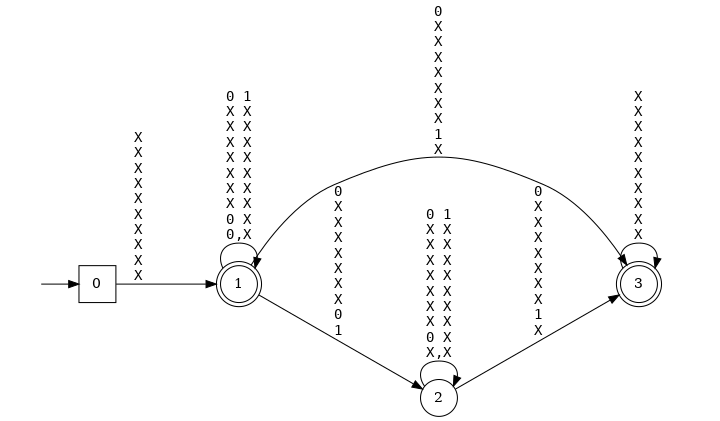
\includegraphics[scale=0.29]{obrazky-figures/exp0_0_mona_aut.png}
            \caption{}
            \label{exp0_img0}
        \end{subfigure}
        \hfil
        \begin{subfigure}{.49\textwidth}
            \centering
            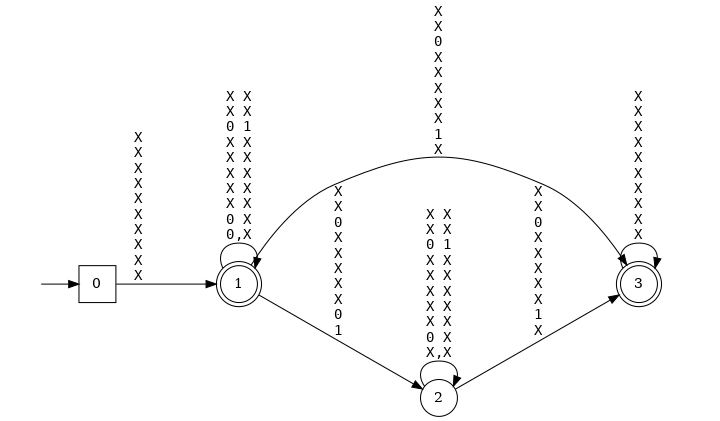
\includegraphics[scale=0.29]{obrazky-figures/exp0_1_mona_aut.png}
            \caption{}
            \label{exp0_img1}
        \end{subfigure}
    \end{subfigure} 
    \vfil
    \begin{subfigure}{.99\textwidth}
        \centering 
        \begin{subfigure}{.49\textwidth}
            \centering
        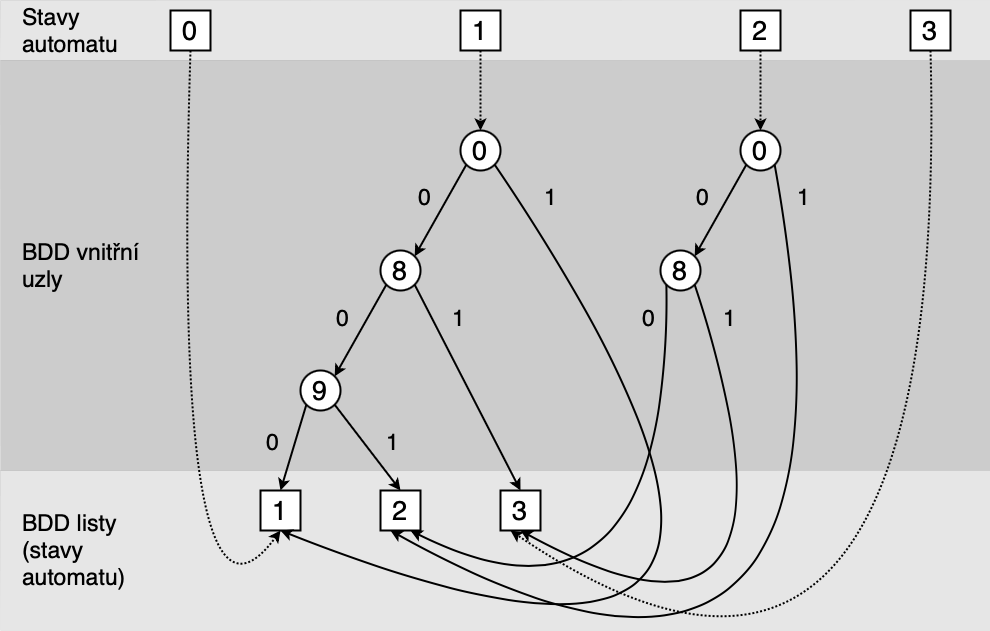
\includegraphics[scale=0.21]{obrazky-figures/exp0_0.png}
            \caption{}
            \label{exp0_img2}
        \end{subfigure}
        \hfil
        \begin{subfigure}{.49\textwidth}
            \centering
            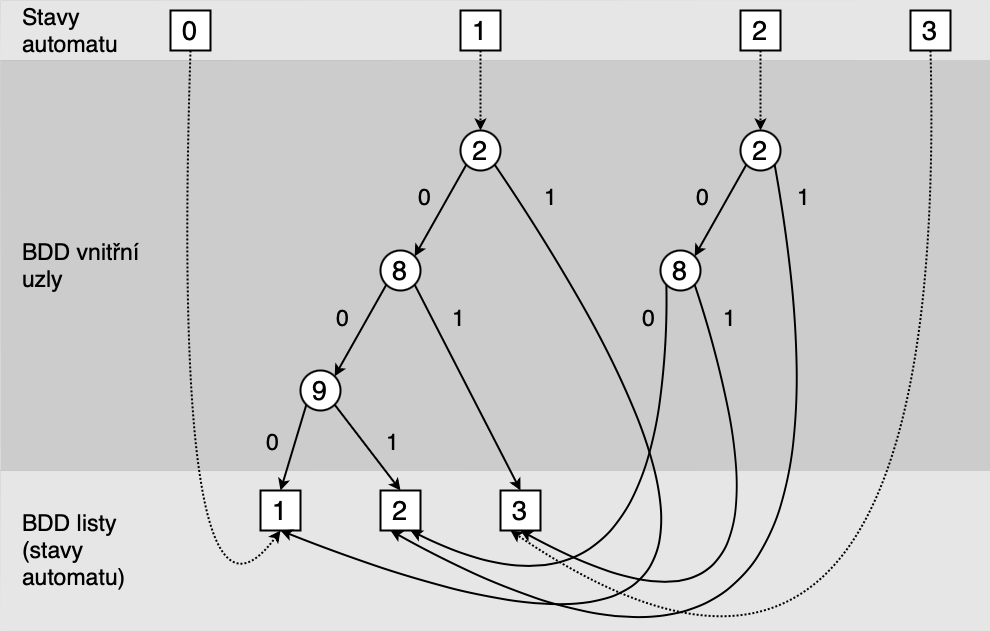
\includegraphics[scale=0.21]{obrazky-figures/exp0_1.png}
            \caption{}
            \label{exp0_img3}
        \end{subfigure}
    \end{subfigure} 
    \vfil
    \begin{subfigure}{.99\textwidth}
        \centering 
        \begin{subfigure}{.49\textwidth}
            \centering
            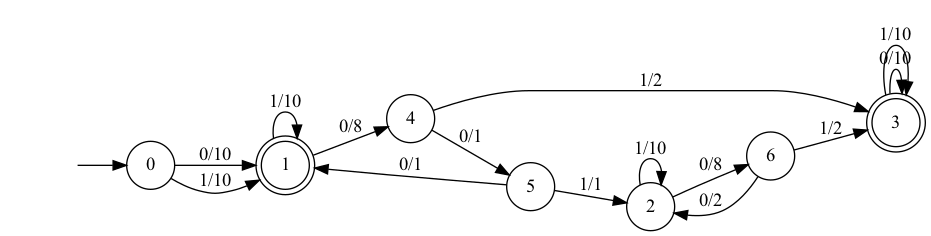
\includegraphics[scale=0.22]{obrazky-figures/exp0_0_we_aut.png}
            \caption{}
            \label{exp0_img4}
        \end{subfigure}
        \hfil
        \begin{subfigure}{.49\textwidth}
            \centering
            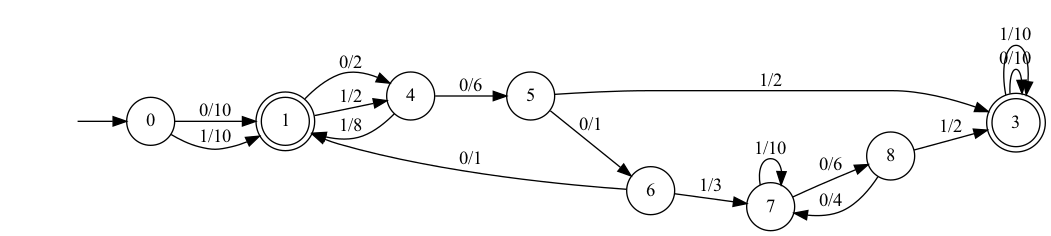
\includegraphics[scale=0.19]{obrazky-figures/exp0_1_we_aut.png}
            \caption{}
            \label{exp0_img5}
        \end{subfigure}
    \end{subfigure} 
    \caption{Porovnání naší a Mona reprezentace automatu. Obrázky \ref{exp0_img0}, \ref{exp0_img2}, \ref{exp0_img4} vizualizují automat pro formuli $X_8 \subseteq X \Rightarrow X_9 \subseteq X$ s pořadím proměnných $X, X_1, X_2, X_3, X_4, X_5, X_6, X_7, X_8, X_9$. Obrázky \ref{exp0_img1}, \ref{exp0_img3}, \ref{exp0_img5} poté ukazují automat pro stejnou formuli, ale s pořadím proměnných $X_1, X_2, X, X_3, X_4, X_5, X_6, X_7, X_8, X_9$. Dále obrázky \ref{exp0_img0}, \ref{exp0_img1} vizualizují Mona reprezentaci převedenou do běžného automatu, obrázky~\ref{exp0_img2},~\ref{exp0_img3} ukazují reálnou podobu Mona reprezentace a obrázky \ref{exp0_img4}, \ref{exp0_img5} vizualizují naši reprezentaci.}
    \label{exp0_img}
\end{figure}

\noindent
s indexem $3$, pak stačí z $s_a$ vytvořit odkaz na BDD uzel odpovídající proměnné $3$ a velikost reprezentace se nezmění. Abychom nastínili tuto situaci, změníme pořadí proměných na $X_1, X_2, X, X_3,$ $X_4,X_5, X_6, X_7, X_8, X_9$ a tím pádem i jejich indexy. U Mona reprezentace se změnily pouze indexy BDD uzlů, viz obrázky \ref{exp0_img1} a \ref{exp0_img3}. V naší reprezentaci, vizualizované obrázkem \ref{exp0_img5}, vznikl navíc jeden stav, ovšem pokud by stav $1$ nebyl koncový, pak by zanikl a počet stavů automatu by zůstal také totožný. Všimněme si, že stav $2$ zanikl, protože nebyl ani koncový, ani z něj nevycházely hrany se symboly $0,1$ do různých stavů. Pokud budeme procházet formuli \ref{exp0_formula} dále a přitom si poznamenávat počty stavů po každé operaci průniku a projekce, dostaneme tabulku \ref{exp0_tbl}, kde vidíme srovnání počtu stavů naší rozhodovací procedůry a nástroje Mona s i bez přidání nevyužité proměnné s indexem $0$, což znamená, že jsme zvětšili o $1$ index všech proměnných a přidali novou na index $0$, kde nová proměnná se nevyskytuje nikde ve formuli, tedy v každém okamžiku má přiřazení $0,1$. Tato proměnná byla přidána, protože v původní formuli \ref{exp0_formula} se v každém kroce přiřazuje do proměnné s indexem $0$, tedy nikdy se nepřeskočí stav úrovně $0$ a nemohli bychom demonstrovat přínos čistě tohoto vylepšení. Ze zmíněné tabulky \ref{exp0_tbl} plyne, že integrace BDD uzlů mezi běžné stavy automatu a také možnost přeskočit stavy úrovně $0$, mají své opodstatnění a představují přínos.

\paragraph{Zhodnocení experimentů.} Experimenty prokázaly, že po stránce počtu generovaných stavů jsme schopni dosáhnout zajímavých výsledků, ovšem doba běhu našeho algoritmu, zejména na formulích vyžadujících hodně minimalizace, je nevyhovující. Jak již bylo zmíněno, řešením by mohlo být vyměnit Brzozowski algoritmus za například nějaký simulační algoritmus, který by byl výrazně složitější na implementaci, ale mohl by přinést dramatické zrychlení.

\chapter{Závěr}
\label{5_zaver}

V této práci jsme popsali teoretické základy rozhodování WS1S, představili vlastní reprezentaci pro rozhodování WS1S, přizpůsobili a optimalizovali pro ni vybrané automatové algoritmy a implementovali ji. Následně jsme s naší implementací provedli experimenty, na základě kterých jsme se naše algoritmy snažili vylepšit a na závěr jsme se porovnali s~nástrojem Mona.

Experimenty jsme provedli na sadě obsahující 196 formulí rozřazených do 11 kategorií. Ukázalo se, že námi použitý Brzozowski minimalizační algoritmus často stavově exploduje, což se podepisuje na časových výsledcích evaluace. Nicméně to otevírá další možnosti zrychlení rozhodovací procedůry čistě tím, že vyměníme minimalizaci za nějakou s nižší časovou složitostí. Změřili jsme i čas běhu představeného algoritmu na testovací sadě formulí, které zvládáme rozhodnout a při odečtení doby běhu naší minimalizace dostáváme, na naší testovací sadě, podobné výsledky jako Mona, tudíž po výměně minimalizačního algoritmu bychom se mohli ještě více přiblížit. Dále z provedených experimentů plyne, že navrhovaná reprezentace je schopna tvořit automaty s méně stavy než Mona. 

V budoucích plánech je implementovat nový minimalizační algoritmus a dále pracovat na dílčích optimalizacích stávajících algoritmů, jako je přidávání globálních proměnných do automatů podle jejich výskytu či lepší práce s prvořádovými proměnnými. Dále jsme se zamýšleli i nad jinými možnostmi reprezentace, a to bez využití BDD kódování přechodů. Například, že bychom měli na hranách přechodové symboly $0,1$ a navíc přechodové značky, které by obsahovaly proměnné do kterých se má přiřadit daný přechodový symbol. Ušetřili bychom stavy, jenž se musí vygenerovat namísto BDD uzlů, ale zároveň získáme okamžitě ekvivalentní informaci o tom do které proměnné je přiřazena $0$ a $1$. Takové automaty by byly v podstatě netederministické, čímž můžeme získat další úsporu. Naznačíme fungování průniku, kde bychom navíc průnikovali značky dvou hran jdoucích z dvojice stavů přes stejný symbol a determinizace, kde naopak hranám, se stejnými symboly jdoucích z množiny stavů, sjednotíme značky.

%===============================================================================

  \fi
  
  % Kompilace po částech (viz výše, nutno odkomentovat)
  % Compilation piecewise (see above, it is necessary to uncomment it)
  %\subfile{projekt-01-uvod-introduction}
  % ...
  %\subfile{chapters/projekt-05-conclusion}


  % Pouzita literatura / Bibliography
  % ----------------------------------------------
\ifslovak
  \makeatletter
  \def\@openbib@code{\addcontentsline{toc}{chapter}{Literatúra}}
  \makeatother
  \bibliographystyle{bib-styles/Pysny/skplain}
\else
  \ifczech
    \makeatletter
    \def\@openbib@code{\addcontentsline{toc}{chapter}{Literatura}}
    \makeatother
    \bibliographystyle{bib-styles/Pysny/czplain}
  \else 
    \makeatletter
    \def\@openbib@code{\addcontentsline{toc}{chapter}{Bibliography}}
    \makeatother
    \bibliographystyle{bib-styles/Pysny/enplain}
  %  \bibliographystyle{alpha}
  \fi
\fi
  \begin{flushleft}
  \bibliography{projekt-20-literatura-bibliography}
  \end{flushleft}

  % vynechani stranky v oboustrannem rezimu
  % Skip the page in the two-sided mode
  \iftwoside
    \cleardoublepage
  \fi

  % Prilohy / Appendices
  % ---------------------------------------------
  \appendix
\ifczech
  \renewcommand{\appendixpagename}{Přílohy}
  \renewcommand{\appendixtocname}{Přílohy}
  \renewcommand{\appendixname}{Příloha}
\fi
\ifslovak
  \renewcommand{\appendixpagename}{Prílohy}
  \renewcommand{\appendixtocname}{Prílohy}
  \renewcommand{\appendixname}{Príloha}
\fi
%  \appendixpage

% vynechani stranky v oboustrannem rezimu
% Skip the page in the two-sided mode
%\iftwoside
%  \cleardoublepage
%\fi
  
\ifslovak
%  \section*{Zoznam príloh}
%  \addcontentsline{toc}{section}{Zoznam príloh}
\else
  \ifczech
%    \section*{Seznam příloh}
%    \addcontentsline{toc}{section}{Seznam příloh}
  \else
%    \section*{List of Appendices}
%    \addcontentsline{toc}{section}{List of Appendices}
  \fi
\fi
  \startcontents[chapters]
  \setlength{\parskip}{0pt} 
  % seznam příloh / list of appendices
  % \printcontents[chapters]{l}{0}{\setcounter{tocdepth}{2}}
  
  \ifODSAZ
    \setlength{\parskip}{0.5\bigskipamount}
  \else
    \setlength{\parskip}{0pt}
  \fi
  
  % vynechani stranky v oboustrannem rezimu
  \iftwoside
    \cleardoublepage
  \fi
  
  % Přílohy / Appendices
  \ifenglish
    .
  \else
    % Tento soubor nahraďte vlastním souborem s přílohami (nadpisy níže jsou pouze pro příklad)

% Umístění obsahu paměťového média do příloh je vhodné konzultovat s vedoucím
%\chapter{Obsah přiloženého paměťového média}

%\chapter{Manuál}

%\chapter{Konfigurační soubor}

%\chapter{RelaxNG Schéma konfiguračního souboru}

%\chapter{Plakát}


  \fi
  
  % Kompilace po částech (viz výše, nutno odkomentovat)
  % Compilation piecewise (see above, it is necessary to uncomment it)
  %\subfile{projekt-30-prilohy-appendices}
  
\end{document}
